\documentclass[12pt, a4paper, onecolumn, oneside, final]{report}

\usepackage{setspace}
\usepackage{csquotes}
\special{papersize=210mm,297mm}
\usepackage[top=3cm,bottom=2.5cm,left=4cm,right=2.5cm]{geometry}
\usepackage{mathptmx}
\usepackage[bahasa]{babel}
\usepackage[backend=biber,style=authoryear]{biblatex}
\usepackage[utf8]{inputenc}
\usepackage{graphicx}
\usepackage{titling}
\usepackage{blindtext}
\usepackage{sectsty}
\usepackage{chngcntr}
\usepackage{etoolbox}
\usepackage{hyperref}
\usepackage{titlesec}
\usepackage{parskip}
\usepackage{tabulary}
\usepackage{longtable}
\usepackage{listings}
\usepackage{xcolor}
\usepackage[titles]{tocloft}
\usepackage{multicol}
\usepackage{tikz,pgfplots}
\usetikzlibrary{matrix}
\usepgfplotslibrary{groupplots}


\hyphenation{sand-box domjudge domserver judgehost test-case di-bang-kit-kan di-se-bab-kan di-ban-ding-kan jud-ge domjudge meng-gu-na-kan me-nye-le-sai-kan pe-rang-kat men-ja-lan-kan di-la-ku-kan on-line ja-wab-an WebAssembly a-kan mem-be-ri-kan ugrade ugserver ugjob http}

\hypersetup{colorlinks=false, pdfborder={0 0 0},}

\renewcommand{\baselinestretch}{1.5}

\renewcommand{\lstlistingname}{Kode.}
\lstdefinestyle{CStyle}{
    belowcaptionskip=1\baselineskip,
    breaklines=true,
    frame=trbl,
    numbers=left,
    xleftmargin=\parindent,
    language=C,
    showstringspaces=false,
    basicstyle=\footnotesize\ttfamily,
    keywordstyle=\bfseries\color{green!40!black},
    commentstyle=\itshape\color{purple!40!black},
    identifierstyle=\color{blue},
    stringstyle=\color{orange},
}
\lstdefinestyle{BashStyle}{
    belowcaptionskip=1\baselineskip,
    breaklines=true,
    frame=trbl,
    numbers=left,
    xleftmargin=\parindent,
    language=Bash,
    showstringspaces=false,
    basicstyle=\footnotesize\ttfamily,
}

\chapterfont{\centering \Large}
\titleformat{\chapter}[display]
    {\Large\centering\bfseries}
    {\chaptertitlename\ \thechapter}{0pt}
        {\Large\bfseries\uppercase}

\setcounter{secnumdepth}{3}

\counterwithin{figure}{section}
\counterwithin{table}{section}

\renewcommand*{\nameyeardelim}{\addcomma\space}
\addbibresource{references.bib}

\DeclareQuoteStyle{bahasa}
    {\textquotedblleft}
    {\textquotedblright}
    [0.05em]
    {\textquotedblleft}
    {\textquotedblright}

\DefineBibliographyStrings{english}{
    and = {\&}
}

\setlength{\cftfignumwidth}{4em}
\setlength{\cfttabnumwidth}{4em}

\begin{document}

    \title{Pengembangan \textit{Autograder Online Judge} Menggunakan PC Pengguna Sebagai \textit{Worker}}
    \date{\today}
    \author{
        Jauhar Arifin \\
        NIM: 13515049
    }

    \pagenumbering{roman}
    \setcounter{page}{0}

    \clearpage
\pagestyle{empty}

\begin{center}
\smallskip
    \Large \bfseries \MakeUppercase{\thetitle}
    \vfill
    \Large Laporan Tugas Akhir
    \vfill
    \large Disusun sebagai syarat kelulusan tingkat sarjana
    \vfill
    \large Oleh
    \Large \theauthor
    \vfill
    \begin{figure}[h]
        \centering
      	
\includegraphics[width=0.15\textwidth]{images/itb-logo}
    \end{figure}
    \vfill
    \large
    \uppercase{
        Program Studi Teknik Informatika \\
        Sekolah Teknik Elektro dan Informatika \\
        Institut Teknologi Bandung
    }

    \thedate
\end{center}
\clearpage


    \pagenumbering{roman}
    \setcounter{page}{0}
    
    \clearpage
\pagestyle{empty}

\begin{center}
\smallskip
    \Large \bfseries \MakeUppercase{\thetitle}
    \vfill
    \Large Laporan Tugas Akhir
    \vfill
    \large Oleh
    \Large \theauthor \\
    \large Program Studi Teknik Informatika \\ Sekolah Teknik Elektro dan Informatika \\ Institut Teknologi Bandung
    \vfill
    \normalsize \normalfont
    \vfill
    Bandung, 26 Desember 2018 \\
    Mengetahui, \\
    Pembimbing,
    \vfill
    \vfill
    \vfill
    Riza Satria Perdana, ST., MT. \\
    NIP. 197006091995121002
\end{center}
\clearpage


    \pagestyle{plain}
    \titleformat*{\section}{\centering\bfseries\Large\MakeUpperCase}

    \clearpage

\chapter*{Lembar Pernyataan}

\par Dengan ini saya menyatakan bahwa:

\begin{enumerate}
    \item Pengerjaan dan penulisan Laporan Tugas Akhir ini dilakukan tanpa menggunakan bantuan yang tidak dibenarkan. 
    \item Segala bentuk kutipan dan acuan terhadap tulisan orang lain yang digunakan di dalam penyusunan laporan tugas akhir ini telah dituliskan dengan baik dan benar. 
    \item Laporan Tugas Akhir ini belum pernah diajukan pada program pendidikan di perguruan tinggi mana pun. 
\end{enumerate}

\par Jika terbukti melanggar hal-hal di atas, saya bersedia dikenakan sanksi sesuai dengan Peraturan Akademik dan Kemahasiswaan Institut Teknologi Bandung bagian Penegakan Norma Akademik dan Kemahasiswaan khususnya Pasal 2.1 dan Pasal 2.2. 

\mbox{}\\
\par Bandung, \thedate \\
\\
\\
\\
\\
\theauthor 

\clearpage

    \clearpage

\chapter*{\uppercase{Abstrak}}
\addcontentsline{toc}{chapter}{\uppercase{Abstrak}}

\begin{center}
    \textbf{\large {\MakeUppercase{\thetitle}}} \\
    \normalsize Oleh \theauthor
\end{center}

\singlespacing
\par \textit{Competitive programming} merupakan kompetisi di bidang \textit{computer science} dimana peserta berlomba menyelesaikan persoalan dengan membuat program sesuai batasan yang ditentukan. Dalam menyelenggarakan kompetisi \textit{competitive programming}, juri menggunakan \textit{autograder} untuk melakukan penilaian. \textit{Autograder} dijalankan pada komputer tertentu yang disebut \textit{worker}. Untuk menjaga kinerja penilaian, diperlukan \textit{worker} dalam jumlah yang besar sehingga diperlukan biaya yang besar pula. 

\par Komputer peserta umumnya memiliki kemampuan yang cukup untuk melakukan penilaian jawaban. Pada tugas akhir ini, komputer peserta digunakan sebagai \textit{worker}. Dengan menggunakan komputer peserta sebagai \textit{worker}, kinerja penilaian dapat meningkat. Setiap peserta memiliki komputer dengan spesifikasi yang berbeda. Untuk menjaga keadilan, solusi peserta dan solusi juri akan dieksekusi pada \textit{worker} dan dibandingkan hasilnya. Kerahasiaan penilaian dijaga dengan melakukan enkripsi pada tingkat aplikasi.

\par Pengujian tugas akhir ini dilakukan dengan menyimulasikan penilaian jawaban peserta oleh \textit{autograder}. Pengujian dilakukan dengan membandingkan kinerja penilaian sistem yang dibangun dengan sistem \textit{online judge} yang bersifat \textit{open source} yaitu \textit{DOMJudge}. Hasil pengujian menyatakan penilaian jawaban dengan memanfaatkan komputer peserta sebagai \textit{worker} meningkatkan kinerja penilaian.

\par Kata kunci: \textit{competitive programming}, \textit{autograder}, \textit{online judge}.

\clearpage
\onehalfspacing
    \clearpage

\chapter*{\uppercase{Kata Pengantar}}
\addcontentsline{toc}{chapter}{\uppercase{Kata Pengantar}}

\par Puji syukur kehadirat Allah SWT, atas limpahan rahmat dan karunia-Nya sehingga penulis dapat menyelesaikan tugas akhir dengan judul "\thetitle". Penulis mengucapkan terima kasih kepada semua pihak yang telah membantu pengerjaan tugas akhir ini. Ucapan terima kasih secara khusus penulis berikan kepada:

\begin{enumerate}
    \item Dosem pembimbing Bapak Riza Satria Perdana, yang telah membimbing dan mengarahkan penulis dalam mengerjakan tugas akhir serta memberikan inspirasi dan pembelajaran yang sangat berarti.
    \item Orang tua dan keluarga yang telah memberikan doa dan dukungannya dalam pengerjaan tugas akhir ini.
    \item Arfinda Ilmania dan seluruh teman-teman Informatika 2015 yang telah memberikan masukan dan dukungan sehingga tugas akhir ini dapat diselesaikan.
    \item Bapak dan ibu dosen informatika yang telah memberikan pembelajaran dan pengalaman yang tak ternilai selama empat tahun masa perkuliahan.
\end{enumerate}

\par Penulis menyadari bahwa tugas akhir ini tidaklah sempurna. Untuk itu penulis ingin meminta maaf dan menerima kritik dan saran yang membangun dan dapat disampaikan melalui alamat email penulis yaitu: jauhararifin10@gmail.com.

\begin{flushright}
Jauhar Arifin
\end{flushright}

\clearpage

    \tableofcontents
    \addcontentsline{toc}{chapter}{\contentsname}\
    \listoffigures
    \addcontentsline{toc}{chapter}{\listfigurename}\
    \listoftables
    \addcontentsline{toc}{chapter}{\listtablename}
    \clearpage

    \titleformat*{\section}{\bfseries\Large}
    \pagenumbering{arabic}
    \setcounter{page}{1}
    \renewcommand{\chaptername}{BAB}
    \renewcommand{\thechapter}{\Roman{chapter}}
    
    \chapter{Pendahuluan}

\section{Latar Belakang}

\par \textit{Competitive programming} merupakan salah satu cabang lomba yang cukup populer di bidang \textit{computer science}. Pada kompetisi \textit{competitive programming}, peserta diminta menyelesaikan persoalan terkait \textit{computer science} yang diberikan oleh juri secara benar dan dalam waktu yang singkat. Beberapa instansi dan organisasi seringkali mengadakan kompetisi ini secara rutin. Perusahaan teknologi besar seperti Google dan Facebook pun seringkali mengadakan kompetisi \textit{competitive programming} secara tahunan. Kompetisi \textit{competitive programming} ditunjang dengan menggunakan sistem \textit{online judge}. Sistem \textit{online judge} tersebut biasanya berupa halaman \textit{web} dimana peserta dapat melihat soal, membuat klarifikasi, mengirimkan jawaban dan melihat \textit{scoreboard}. Sistem \textit{online judge} yang populer pada saat ini adalah Codeforces, URI \textit{Online Judge} (\cite{uriojpaper}), Uva, dan SPOJ.

\par Di dalam sistem \textit{online judge}, terdapat sistem \textit{autograder} yang digunakan untuk menilai jawaban peserta. Jawaban peserta yang berupa \textit{source code} bahasa pemrograman akan dinilai kebenarannya oleh sistem \textit{autograder} dengan cara melakukan kompilasi pada kode tersebut kemudian mengeksekusi program hasil kompilasi dengan \textit{test-case} yang sudah disiapkan oleh pembuat soal. Dengan menggunakan \textit{autograder}, penilaian jawaban peserta dapat dilakukan secara otomatis dan keterlibatan manusia menjadi lebih sedikit. Untuk meningkatkan jumlah jawaban peserta yang dapat dinilai dalam satuan waktu, biasanya juri menyiapkan lebih dari satu komputer yang menjalankan sistem \textit{autograder}. Dalam menjalankan sistem \textit{autograder} pada lebih dari satu komputer diperlukan komputer dengan spesifikasi yang sama untuk menjaga keadilan dalam penilaian.

\par Saat ini, hampir semua kompetisi \textit{competitive programming} menggunakan sistem \textit{autograder}. Kebanyakan dari kompetisi tersebut juga telah menggunakan lebih dari satu \textit{autograder} yang berjalan. Meskipun begitu, karena banyaknya peserta yang mengikuti kompetisi tersebut, seringkali jumlah \textit{autograder} yang disiapkan oleh juri kurang dan mengakibatkan jawaban peserta tidak dapat dinilai secara cepat. Penggunaan sistem \textit{autograder} yang banyak juga menghabiskan banyak biaya karena perlu menyewa komputer dengan kinerja yang cukup tinggi untuk menjalankan sistem \textit{autograder} tersebut. Oleh karena itu, diperlukan sistem penilaian baru yang dapat mengurangi biaya pengadaan infrastruktur guna menjalankan sistem \textit{autograder}.

\par Dalam mengikuti kompetisi \textit{competitive programming}, peserta umumnya menggunakan komputer pribadinya untuk menulis program yang digunakan untuk menyelesaikan soal yang diberikan. Setiap komputer yang digunakan oleh peserta umumnya memiliki spesifikasi yang cukup untuk melakukan kompilasi pada \textit{source code} yang ditulis oleh peserta dan melakukan eksekusi program hasil kompilasi tersebut. Oleh sebab itu, komputer peserta berpotensi untuk menjadi infrastruktur yang dapat digunakan untuk melakukan penilaian program oleh \textit{autograder}.

\section{Rumusan Masalah}

\par Masalah yang ingin diselesaikan dalam Tugas Akhir ini adalah:
\begin{enumerate}

	\item Sistem \textit{autograder} yang sering digunakan saat ini melakukan penilaian terhadap kode peserta dengan melakukan kompilasi dan eksekusi pada komputer yang disediakan oleh juri. Komputer yang digunakan oleh peserta kompetisi \textit{competitive programming} memiliki kemampuan untuk menjalankan sistem \textit{autograder}. Bagaimana memanfaatkan komputer peserta tersebut untuk menjalankan sistem \textit{autograder} untuk menilai jawaban peserta saat kompetisi sedang berlangsung.
	
	\item Dalam menjalankan sistem \textit{autograder}, aspek keamanan, keadilan dan kinerja perlu diperhatikan. Bagaimana menjaga keamanan, keadilan dan kinerja dari sistem \textit{autograder} yang berjalan pada komputer peserta.

\end{enumerate}

\section{Tujuan}

\par Tujuan yang ingin dicapai dari Tugas Akhir ini adalah menciptakan sistem \textit{autograder} yang dapat berjalan pada komputer pengguna dengan aman dan adil.

\section{Batasan Masalah}

\par Pada pengerjaan Tugas Akhir ini, diasumsikan seluruh peserta yang menggunakan perangkat lunak ini memiliki komputer dengan spesifikasi yang cukup untuk menjalankan sistem \textit{autograder} dan memiliki sistem operasi berbasis Linux. Perangkat lunak yang dibangun untuk menjalankan sistem \textit{autograder} hanya mencakup sistem \textit{autograder} untuk domain \textit{competitive programming} saja.

\section{Metodologi}

\par Metodologi yang dilakukan dalam pengerjaan Tugas Akhir ini adalah:
\begin{enumerate}

	\item Menganalisis dan Mendesain Sistem \textit{Autograder} \\ Pada tahap ini akan dilakukan analisis terhadap teknik pembuatan sistem \textit{autograder} beserta aspek-aspek yang perlu diperhatikan dalam melakukan pengembangan sistem \textit{autograder}. Selain itu, pada tahap ini juga dihasilkan metode yang akan digunakan untuk mengembangkan sistem \textit{autograder} yang dapat berjalan pada komputer peserta.
	
	\item Desain dan Analisis Perangkat Lunak \\ Pada tahap ini akan dilakukan analisis terhadap kebutuhan perangkat lunak beserta membuat desain perangkat lunak yang akan diimplementasikan.
	
	\item Implementasi Pengembangan Perangkat Lunak \\ Pada tahap ini, implementasi dari pengembangan perangkat lunak akan dilakukan berdasarkan desain yang sudah dibuat pada tahap sebelumnya.
	
	\item Pengujian \\ Perangkat lunak yang telah dihasilkan diuji pada tahap ini sesuai dengan kebutuhan yang telah didefinisikan.
	
	\item Penarikan Kesimpulan \\ Pada tahap ini, hasil pengujian akan digunakan untuk melakukan penarikan kesimpulan.

\end{enumerate}

\section{Jadwal Pelaksanaan Tugas Akhir}

\par Rencana kegiatan dan jadwal pengerjaan Tugas Akhir 1 hingga sidang tugas akhir dapat dilihat pada Tabel \ref{tab:final-project-schedule} berikut.

\begin{longtable}{|p{.33\textwidth}|p{.33\textwidth}|p{.33\textwidth}|}
	\caption{Tabel Jadwal Pengerjaan Tugas Akhir}
	\label{tab:final-project-schedule}
	\endfirsthead
	\endhead
	\hline
	Tanggal & Kegiatan & \textit{Deliverable} \\\hline
	1 Oktober 2018 - 28 Oktober 2018 & Melakukan studi literatur & Studi Literatur (Bab 2) \\ \hline
	29 Oktober 2018 - 12 November 2018 & Penulisan Bab 1 & Pendahuluan (Bab 1) \\ \hline
	13 November 2018 - 30 November 2018 & Mendesain arsitektur perangkat lunak yang akan dibangun & Rancangan arsitektur perangkat lunak \\ \hline
	1 Desember 2018 - 8 Desember 2018 & Penulisan Bab 3 & Rencana Penyelesaian Masalah (Bab 3) \\ \hline
	9 Desember 2018 - 15 Desember 2018 & Melakukan revisi Bab 1 - 3 & Draft buku TA 1 \\ \hline
	16 Desember 2018 - 22 Desember 2018 & Mengumpulkan buku TA 1 & Buku TA 1 \\ \hline
	14 Januari 2019 & Melakukan seminar TA 1 & Seminar TA 1 \\ \hline
	1 Januari 2019 - 31 Maret 2019 & Melakukan implementasi dari perangkat lunak yang dibangun & Perangkat lunak \\ \hline
	1 April 2019 - 15 April 2019 & Melakukan pengujian perangkat lunak & Hasil pengujian perangkat lunak \\ \hline
	16 April 2019 - 30 April 2019 & Menyelesaikan laporan tugas akhir & Laporan tugas akhir \\ \hline
	19 Mei 2019 & Seminar TA 2 & Presentasi seminar TA II, laporan tugas akhir hasil revisi \\ \hline
	27 Mei 2019 & Sidang TA & - \\ \hline
	3 Juni 2019 & Mengumpulkan buku laporan tugas akhir & Buku laporan tugas akhir \\
	\hline
\end{longtable}

    \chapter{Studi Literatur}

\par Pada bab ini dipaparkan hasil studi literatur terkait dengan sistem \textit{competitive programming}. Studi literatur yang dilakukan adalah terkait sistem yang digunakan dalam menyelenggarakan kompetisi \textit{competitive programming}, \textit{online judging system}, \textit{autograder} dan metode yang digunakan dalam melakukan grading.

\section{\textit{Competitive Programming}}

\par \textit{Competitive programming} merupakan sebuah kompetisi dimana peserta dari kompetisi tersebut diminta menyelesaikan suatu permasalahan pada bidang \textit{computer science} secara cepat dan tepat. Pada kompetisi \textit{competitive programming}, peserta akan diberikan permasalahan \textit{computer science} yang sudah pernah diselesaikan dan bukan permasalahan riset yang solusinya masih belum ditemukan (\cite{halimsfcp3}). Untuk setiap persoalan yang diberikan, peserta diminta untuk menyelesaikan masalah tersebut dengan membuat program dalam bahasa pemrograman yang diizinkan oleh juri. Program yang dibuat oleh peserta harus memenuhi batasan yang dibuat oleh juri seperti waktu eksekusi, kebutuhan memori, dan ukuran program.
\par Pada kompetisi \textit{competitive programming}, program yang telah dibuat oleh peserta akan dinilai dengan suatu metode tertentu. Umumnya penilaian yang dilakukan mencakup kebenaran program dan waktu pengumpulan program, akan tetapi terdapat beberapa metode penilaian lain yang dapat dilakukan. Beberapa standar metode telah digunakan untuk melakukan penilaian jawaban dalam kompetisi \textit{competitive programming}, diantaranya adalah standar IOI dan ICPC. Beberapa kompetisi \textit{competitive programming} diselenggarakan oleh suatu organisasi, contohnya adalah ICPC yang diselenggarakan oleh ICPC Foundation (\cite{abouticpc}), dan IOI (International Olympiad in Informatics) yang diselenggarakan oleh IOI Community (\cite{ioiorg}). Selain itu, terdapat juga kompetisi \textit{competitive programming} yang diselenggarakan oleh suatu perusahaan seperti Google Code Jam yang diselenggarakan oleh Google dan Facebook HackerCup yang diselenggarakan oleh Facebook.
\par Kompetisi \textit{competitive programming} pada tingkat perguruan tinggi biasanya mengikuti standar ICPC. Beberapa kompetisi yang mengikuti standar ini adalah Gemastik, Compfest, Vocomfest, INC, dan ACM-ICPC. Pada standar ICPC, setiap peserta akan bekerja dalam sebuah tim yang terdiri dari tiga peserta. Tiap tim akan diberikan soal yang sama. Seluruh tim akan mulai mengerjakan soal secara bersama-sama. Program yang telah dibuat oleh sebuah tim akan dikirimkan ke sistem untuk dinilai. Penilaian dilakukan secara otomatis pada sistem yang disebut \textit{online judge}. Pada sistem \textit{online judge} penilaian dilakukan dengan menggunakan sebuah \textit{autograder} yang berjalan di dalam sistem \textit{online judge}, \textit{autograder} akan menjalankan program yang dikirimkan oleh peserta dan menentukan apakah program tersebut benar atau salah. Setiap program yang dikirimkan oleh peserta hanya dapat bernilai benar atau salah. Setiap tim yang mengirimkan program yang salah akan mendapatkan penalti waktu. Nilai total dari sebuah tim dihitung dari jumlah soal yang berhasil dikerjakan oleh tim tersebut. Jika terdapat dua buah tim yang menyelesaikan soal dengan jumlah yang sama akan dihitung jumlah penalti waktunya untuk menentukan tim yang nilainya lebih tinggi (\cite{wfrules}).
\par Selain standar ICPC, terdapat standar lain yang biasa digunakan untuk tingkat sekolah menengah atas yaitu standar IOI. Pada standar IOI setiap peserta bekerja secara individu dan mendapatkan soal yang sama. Berbeda dengan standar ICPC, pada standar IOI setiap soal memiliki beberapa \textit{subtask} dengan nilai tertentu. Peserta dapat menyelesaikan soal secara parsial dan mendapatkan nilai berdasarkan total dari \textit{subtask} yang berhasil diselesaikan dengan benar pada soal tersebut (\cite{ioi2017}).
\par Terdapat jenis \textit{competitive programming} lain yang tidak memiliki standar tertentu, misalnya Google Code Jam dan Codeforces. Pada kompetisi Google Code Jam, sistem tidak melakukan penilaian dengan menjalankan program yang dibuat oleh peserta, melainkan hanya meminta jawaban dari peserta dalam bentuk file output yang sudah dihasilkan oleh program peserta yang dijalankan di komputer peserta sendiri. Pada kompetisi Codeforces, sistem penilaian memiliki banyak perbedaan dengan sistem penilaian lain. Pada kompetisi ini, setiap soal memiliki nilai yang berbeda dan nilainya akan terus berkurang selama kompetisi berlangsung. Selain itu, pada kompetisi Codeforces peserta dapat melakukan hack pada program yang telah dikirimkan peserta lain (\cite{cfrules}).

\section{\textit{Online Judge} System}

\par \textit{Online judge} merupakan suatu \textit{platform} yang digunakan untuk menyelenggarakan kompetisi \textit{competitive programming}. Peserta kompetisi menggunakan sistem \textit{online judge} untuk mengakses soal dan mengirimkan jawaban atau program yang telah dibuat. \textit{Online judge} system akan melakukan kompilasi pada kode yang dikirimkan peserta lalu mengevaluasi program yang dihasilkan dengan \textit{test-case} tertentu untuk menilai jawaban peserta tersebut (\cite{wasikojsurvey}). Selain itu sistem \textit{online judge} juga memiliki beberapa fungsi lain diantaranya adalah untuk melihat \textit{scoreboard} dan melakukan klarifikasi pada soal. Umumnya sistem \textit{online judge} berupa halaman \textit{web} yang berisi antar muka untuk membaca soal dan mengirimkan jawaban dari soal tersebut. Gambar \ref{fig:codeforces} memperlihatkan contoh halaman soal dari sistem \textit{online judge} yang cukup populer yaitu Codeforces.

\begin{figure}
	\centering
	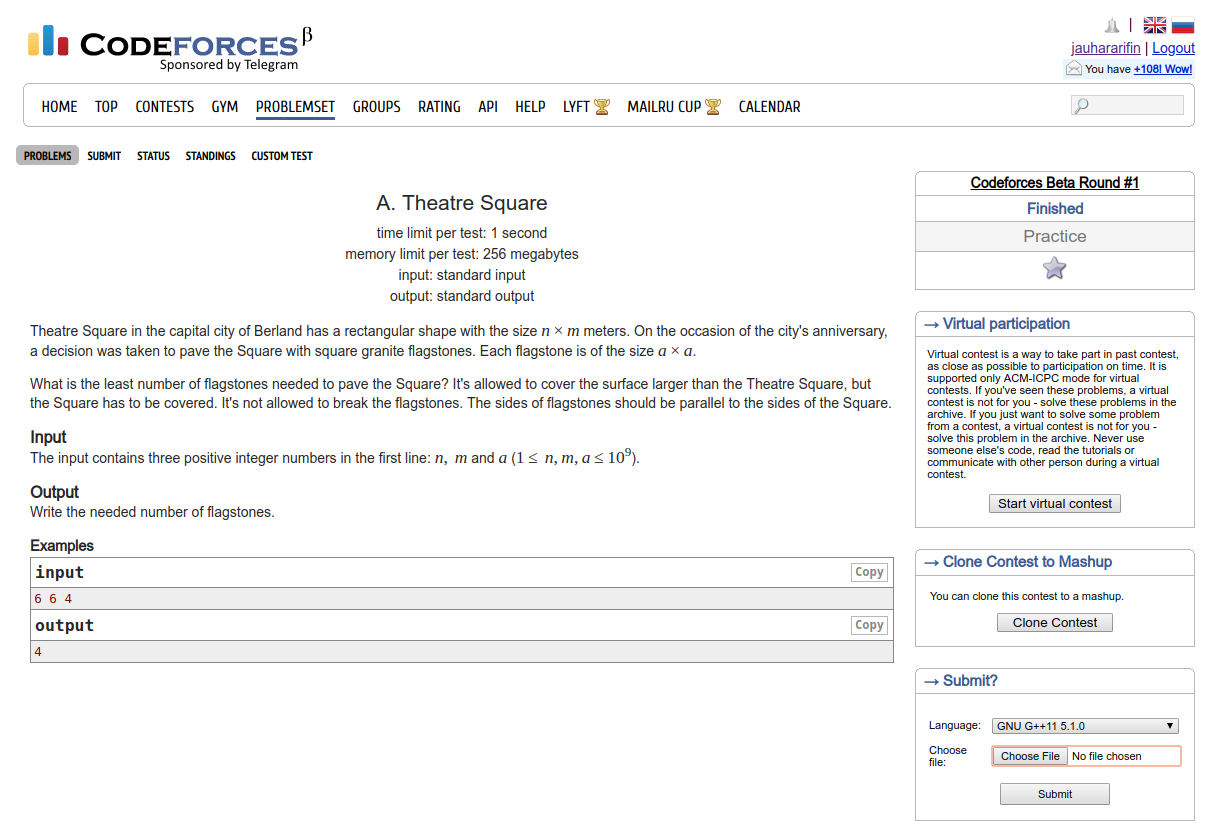
\includegraphics[width=\textwidth]{images/codeforces}
	\caption{Contoh Sistem \textit{Online Judge} : Codeforces.}
	\label{fig:codeforces}
\end{figure}

\par Beberapa organisasi memiliki \textit{online judge} yang secara publik dapat diakses, diantaranya adalah: URI \textit{Online Judge}, TOKI \textit{Online Judge}, Codeforces, Uva, SPOJ, dan lain sebagainya. \textit{Online judge} yang bersifat publik ini biasanya memiliki beberapa soal-soal yang dapat digunakan untuk latihan dan dapat dikerjakan tanpa harus berkompetisi dengan peserta lain. Pada URI \textit{Online Judge} terdapat fitur tambahan seperti forum dan \textit{rewarding system} (\cite{uriojpaper}). Terdapat beberapa sistem \textit{online judge} yang bersifat \textit{open source} seperti Mooshak, Judgels, dan DomJudge. Sistem \textit{online judge} yang bersifat open source biasanya digunakan untuk oleh beberapa instansi seperti universitas untuk membuat kompetisi \textit{competitive programming} yang bersifat privat seperti Gemastik, Compfest, Vocompfest, Arkavidia, dan INC.

\section{\textit{Autograder}}

\par \textit{Autograder} merupakan suatu aplikasi yang digunakan untuk melakukan kompilasi, eksekusi dan menilai sebuah \textit{source code} (\cite{danutamalms}). \textit{Autograder} digunakan dalam sistem \textit{online judge} untuk menilai kebenaran suatu \textit{source code}. Umumnya \textit{autograder} akan melakukan kompilasi pada \textit{source code} yang dikirimkan oleh peserta pada kompetisi \textit{competitive programming}. Hasil kompilasi dari kode peserta tersebut akan di-test dengan menggunakan \textit{test-case} rahasia yang telah dibuat oleh juri atau \textit{problem setter}. Setelah melalui pengetesan, program akan dinilai berdasarkan hasil tes tersebut. Gambar \ref{fig:grading-process} menjelaskan alur penilaian sebuah \textit{source code} yang dikirimkan peserta.

\begin{figure}
	\centering
	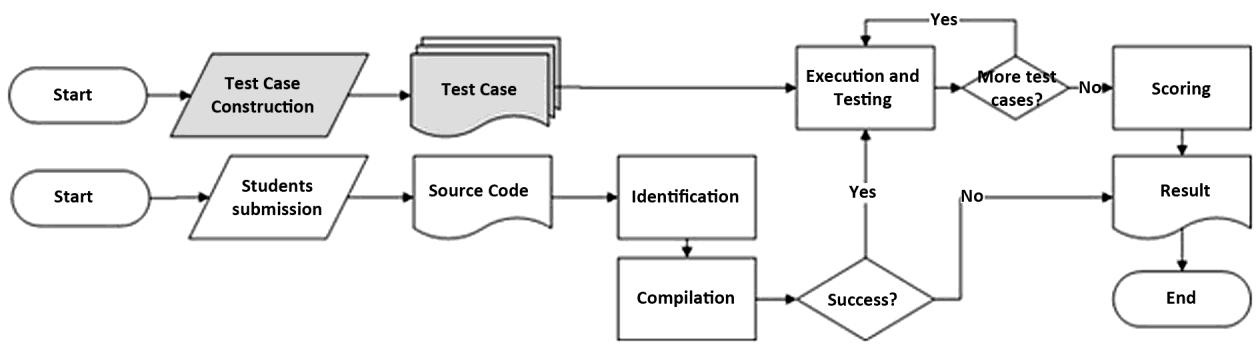
\includegraphics[width=\textwidth]{images/grading-process}
	\caption{Proses penilaian program peserta (\cite{danutamalms}}
	\label{fig:grading-process}
\end{figure}

\par Seluruh proses penilaian sebuah \textit{source code} peserta membutuhkan waktu tiga menit jika dilakukan secara manual, sedangkan hanya membutuhkan waktu sepuluh detik dengan menggunakan \textit{autograder} (\cite{danutamalms}). Dengan menggunakan \textit{autograder}, peserta kompetisi \textit{competitive programming} dapat menerima \textit{feedback} dengan lebih cepat dan mengurangi pekerjaan yang harus dilakukan oleh juri.

\par Terdapat banyak hal yang harus diperhatikan dalam membangun sistem \textit{online judge} dengan menggunakan \textit{autograder}. Salah satu permasalahan yang harus dihadapi dalam membangun \textit{autograder} adalah masalah keamanan sistem. Sistem \textit{autograder} harus dapat bertahan terhadap serangan yang mungkin dilakukan oleh peserta. Beberapa serangan yang mungkin dilakukan oleh peserta adalah mengirimkan \textit{source code} yang memiliki waktu kompilasi yang sangat lama dan membebani sistem, membuat kode yang dapat mengubah atau merusah lingkungan testing \textit{autograder}, dan mengakses \textit{resource} dari \textit{autograder} yang tidak diizinkan oleh sistem (\cite{wasikojsurvey}). Metode yang mungkin dilakukan untuk mengatasi masalah keamanan tersebut adalah dengan melakukan \textit{sandboxing}. \textit{Sandboxing} merupakan teknik mengisolasi suatu eksekusi program sehingga tidak mengganggu lingkungannya. Metode \textit{sandboxing} yang populer untuk masalah ini adalah dengan menggunakan \textit{virtualization} seperti KVM, atau menggunakan \textit{container} seperti LXC dan Docker.

\par Hal lain yang perlu diperhatikan dalam membangun \textit{autograder} adalah aspek \textit{fairness}. Waktu eksekusi program perlu diukur dengan tepat untuk menciptakan sistem yang adil. Waktu eksekusi program yang sama dengan input yang sama dapat memiliki nilai yang berbeda bergantung beberapa faktor seperti kecepatan CPU, ukuran RAM, dan lain sebagainya. Waktu pengukuran sebuah program dalam sistem \textit{autograder} biasanya dilakukan dalam hitungan milidetik. Beberapa metode yang dapat digunakan untuk mengukur waktu pemrosesan adalah dengan melakukan analisis pada \textit{hardware performance}, \textit{code instrumentation}, atau \textit{code sampling} (\cite{wasikojsurvey}). Umumnya \textit{autograder} dalam sebuah sistem \textit{online judge} memiliki banyak \textit{worker} untuk meningkatnya banyaknya program yang dapat dinilai dalam satuan waktu. \textit{Autograder} ini dapat dijalankan di komputer yang berbeda, dan dapat memiliki kinerja yang berbeda. Oleh karena itu, pengukuran waktu sangat penting dalam sistem \textit{autograder} untuk meningkatkan \textit{fairness} dari sistem.

\section{\textit{Containerization}}

\par Secara singkat \textit{container} merupakan teknologi virtualisasi program pada tingkat sistem operasi, berbeda dengan teknik virutalisasi menggunakan \textit{hypervisor} yang bekerja pada tingkat \textit{hardware} (\cite{merkeldocker}). \textit{Container} bekerja seperti \textit{virtual machine} yang dapat memberikan isolasi terhadap program yang berjalan. Pada \textit{virtual machine}, virtualisasi terjadi pada tingkat \textit{hardware} sehingga pengguna perlu menginstall sistem operasi pada lingkungan yang terisolasi untuk dapat menjalankan program. Pada \textit{container}, pengguna tidak perlu menginstall sistem operasi karena virtualisasi terjadi pada tingkat \textit{software} sehingga sistem operasi dari \textit{host} dapat digunakan dalam \textit{container}. Hal tersebut membuat \textit{container} lebih ringan dibandingkan \textit{virtual machine} karena tidak ada kerja tambahan untuk menjalankan sistem operasi baru. Gambar \ref{fig:docker-architecture} mengilustrasikan arsitektur salah satu \textit{container} yang populer yaitu Docker.

\begin{figure}
	\centering
	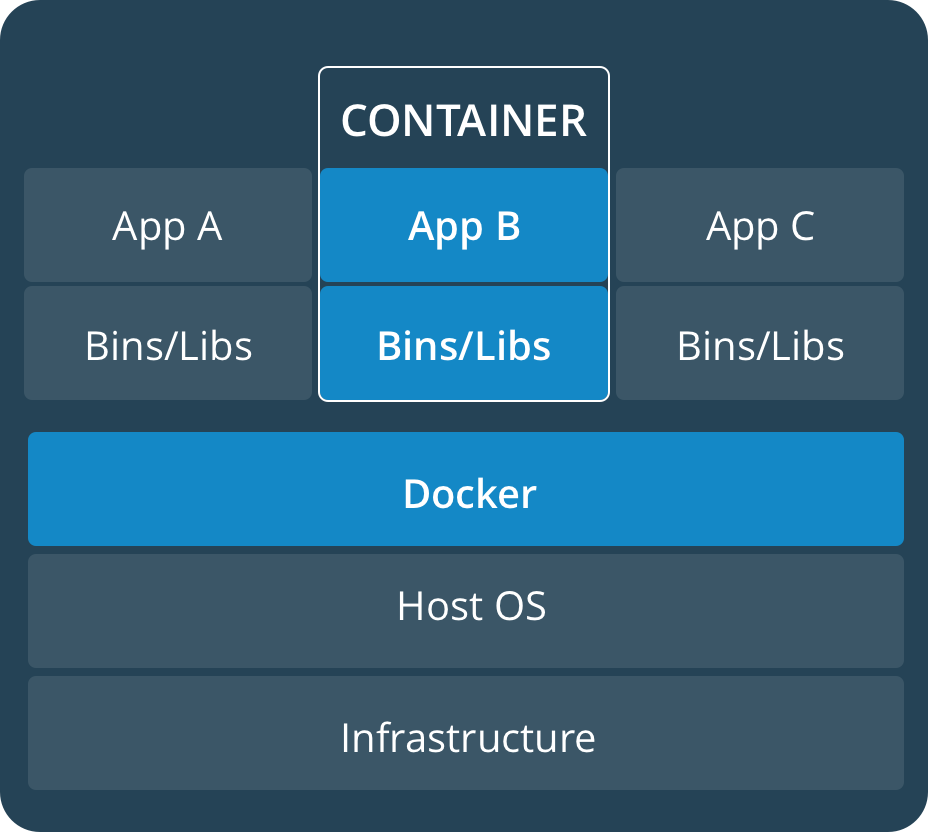
\includegraphics[width=0.5\textwidth]{images/docker-architecture}
	\caption{Arsitektur \textit{container} pada Docker (\cite{dockerdocs}).}
	\label{fig:docker-architecture}
\end{figure}

\par Pada \textit{linux}, teknologi mungkin dilakukan karena adanya beberapa fitur dari \textit{linux} yaitu: \textit{chroot}, \textit{cgroup} dan \textit{namespace}. \textit{Cgroup} dapat memberikan isolasi \textit{file system} terhadap suatu program yang berjalan pada \textit{linux}. \textit{Cgroup} dapat memberikan batasan \textit{resource} kepada suatu program yang berjalan pada \textit{linux}. \textit{Namespace} dapat memberikan isolasi pada program sehingga program dalam suatu lingkungan tidak dapat mengetahui adanya program pada lingkungan lain. Terdapat beberapa perangkat lunak yang menawarkan teknologi \textit{containerization} ini, yang populer diantaranya adalah: Docker dan LXC. Dengan menggunakan Docker atau LXC, pengguna dapat membuat suatu lingkungan yang tersiolasi untuk menjalankan suatu program tertentu tanpa mengganggu lingkungan diluar lingkungannya. Docker memberikan \textit{API} yang lebih \textit{high-level} dibandingkan dengan LXC, dan memiliki banyak fitur yang dapat digunakan untuk mengelola \textit{container}. Docker biasanya digunakan sebagai \textit{platform} untuk mendeploy aplikasi.

\par Teknologi \textit{container} dapat digunakan untuk melakukan penilaian terhadap kode program yang dikirimkan oleh peserta kompetisi \textit{competitive programming}. Dengan menggunakan \textit{container}, program yang dijalankan dapat diisolasi sehingga tidak membahayakan lingkungan. Selain itu, \textit{resource} seperti \textit{CPU usage}, \textit{memory}, \textit{storage}, dan IO pada \textit{container} dapat dibatasi sehingga tidak mengganggu program lain yang sedang berjalan pada lingkungan di luar \textit{container} (\cite{merkeldocker}).

\section{\textit{Chroot}}

\par \textit{Chroot} merupakan \textit{system call} pada sistem operasi yang berbasis \textit{linux} atau \textit{unix}. \textit{System call} ini dapat mengubah \textit{root file system} ke direktori target tertentu kemudian menjalankan program. Program yang dijalankan seakan-akan memiliki direktori \textit{root} sebagai direktori yang dispesifikasi pada waktu pemanggilan \textit{system call} \textit{chroot}. Dengan mengguakan cara ini, program yang dijalankan dalam \textit{chroot} hanya dapat mengakses \textit{file system} yang berada pada direktori target saja dan mengurangi kemungkinan serangan yang mungkin dilakukan pada \textit{file system} asli (\cite{lessardchroot}). Dengan menggunakan \textit{chroot}, pengguna dapat mengatur \textit{library} apa saja yang dapat digunakan oleh program yang berjalan dalam lingkungan \textit{chroot}. Hal ini dapat menjadi merepotkan karena pengguna perlu memasukkan semua \textit{library} yang dibutuhkan ke dalam \textit{file system} \textit{chroot}. Teknologi \textit{container} memanfaatkan \textit{chroot} untuk mengisolasi \textit{file system} yang dapat diakses oleh program yang berjalan pada \textit{container}.

\par Meskipun \textit{chroot} memberikan penghalang pada aplikasi yang berada dalam lingkungan \textit{chroot} untuk mengakses \textit{file system} yang berada di luar lingkungan direktori target, \textit{chroot} masih memiliki kelemahan. Jika aplikasi yang berjalan pada lingkungan \textit{chroot} memiliki root permission, maka aplikasi tersebut dapat dengan mudah keluar dari lingkungan \textit{chroot}. Terdapat beberapa cara untuk meningkatkan keamanan \textit{chroot} sehingga program yang berjalan di dalam \textit{chroot} sulit  untuk keluar dari lingkungan tersebut.

\par Salah satu cara untuk meningkatkan keamanan pada lingkungan \textit{chroot} adalah dengan memasukkan file yang hanya dibutuhkan oleh program saja. Sebagai contoh, jika program membutuhkan daftar user yang berada dalam sistem, di dalam linkungan \textit{chroot} perlu ada file /etc/passwd untuk mendapatkan informasi ini. Akan tetapi, file /etc/shadow tidak perlu dimasukkan ke dalam \textit{file system} \textit{chroot} karena mengandung informasi rahasia yang tidak diperlukan oleh program yang berada dalam lingkungan \textit{chroot}.

\par Cara kedua untuk meningkatkan keamanan lingkungan \textit{chroot} adalah dengan tidak memberikan akses \textit{root} kepada program yang berjalan di dalam \textit{chroot}. Terdapat beberapa serangan yang memungkinkan program dalam lingkungan \textit{chroot} untuk keluar dari lingkungan \textit{chroot} jika memiliki akses \textit{root}. Untuk menghindari jenis serangan ini, sebaiknya program yang berjalan di dalam lingkungan \textit{chroot} dibuat agar tidak mungkin mendapatkan akses \textit{root}. Tidak memberikan akses \textit{root} kepada program akan mengurangi kemungkinan adanya serangan. Akan tetapi, meskipun tidak memberikan akses \textit{root}, masih terdapat beberapa serangan yang memungkinkan program membangkitkan akses \textit{root} tanpa memiliki akses \textit{root} pada saat dijalankan.

\par Untuk meningkatkan keamanan pada lingkungan \textit{chroot}, sebaiknya tidak memasukkan \textit{hard link} ke dalam \textit{file system} \textit{chroot}. \textit{Hard link} yang mengacu pada file di luar lingkungan \textit{chroot} akan mengurangi keamanan \textit{chroot} karena memungkinkan program yang berada di dalam lingkungan \textit{chroot} untuk mengakses file yang berada di luar lingkungan \textit{chroot}.

\section{\textit{Cgroup}}

\par \textit{Cgroup} merupakan fitur pada \textit{linux} yang dapat digunakan untuk membatasi \textit{resource} yang digunakan oleh suatu kelompok program (\cite{wfeltervmcontainer}). \textit{Resource} yang dimaksud di sini adalah \textit{CPU usage}, \textit{memory usage}, \textit{disk IO} dan \textit{network IO}. Dengan menggunakan \textit{cgroup}, sebuah program yang dibatasi \textit{resource}-nya tidak akan mengganggu program lain dengan cara menghabiskan \textit{resource}. Fitur \textit{cgroup} dimanfaatkan oleh teknologi \textit{container} untuk membatasi \textit{resource} pada sebuah \textit{container} sehingga tidak membebani program lain di luar \textit{container}. Pada \textit{container}, umumnya \textit{cgroup} digunakan untuk membatasi CPU dan memori yang digunakan oleh program-program yang berjalan di dalam \textit{container}. \textit{Cgroup} dapat memberhentikan program di dalam \textit{container} jika telah menggunakan \textit{resource} yang berlebihan.

\section{\textit{Namespace}}

\par Dengan menggunakan \textit{chroot} dan \textit{cgroup}, sebuah program dapat diisolasi sehingga memiliki \textit{resource} dan \textit{file system} sendiri yang terpisah dari program-program lain yang berjalan pada \textit{host operating system}. Meskipun begitu, program yang terisolasi ini masih dapat melihat proses apa saja yang sedang berjalan pada sistem operasi karena program yang berjalan di dalam \textit{chroot} dan \textit{cgroup} masih menggunakan sistem operasi yang sama dan menggunakan kernel yang sama. \textit{Linux} memiliki fitur \textit{namespace} yang memberikan isolasi kepada program terhadap masalah ini. Dengan menggunakan \textit{namespace}, sebuah program dapat berjalan di atas \textit{namespace} tertentu dan hanya dapat mengetahui program lain yang berada di dalam \textit{namespace} yang sama. Pada \textit{container}, \textit{namespace} digunakan sehingga program yang berjalan di dalam \textit{container} hanya mengetahui program yang berada di dalam \textit{container} tersebut dan tidak dapat mengetahui program yang sedang berjalan pada \textit{host} OS-nya (\cite{wfeltervmcontainer}).

\par Selain isolasi program, \textit{namespace} juga memberikan isolasi pada hal lain seperti \textit{network}, \textit{mount}, \textit{cgroup}, \textit{user}, dan lain sebagainya. Dengan memberikan isolasi pada \textit{network}, program yang berada di dalam \textit{container} dapat membuka \textit{port} yang sama seperti program lain yang berada di \textit{container} lain. Dengan menggaunakan isolasi pada \textit{user}, \textit{user} yang ada di dalam \textit{container} tidak dapat diketahui oleh \textit{container} lain.

\section{Kernel \textit{Virtual Machine}}

\par \textit{Virtual machine} memberikan teknik virtualisasi yang berbeda dengan \textit{container}. \textit{Container} berjalan pada \textit{level} sistem operasi sedangkan \textit{virtual machine} berjalan pada \textit{level} \textit{hardware}. Pada \textit{container}, fitur-fitur dari \textit{linux} digunakan untuk mendukung virtualisasi dan isolasi program, sedangkan pada \textit{virtual machine} digunakan \textit{hypervisor} untuk melakukan virtualisasi. Dengan menggunakan \textit{virtual machine}, pengguna dapat menjalankan lebih dari satu sistem operasi berbeda di dalam komputer yang sama. Hal ini berbeda dengan \textit{container} yang hanya dapat menjalankan satu sistem operasi saja. KVM merupakan fitur dari \textit{linux} yang memungkinkan \textit{linux} menjadi \textit{hypervisor} dan menjalankan \textit{guest OS} di dalam proses \textit{linux} (\cite{wfeltervmcontainer}).

\par KVM memiliki fitur yang mirip dengan \textit{container}. Program yang berjalan di dalam \textit{virtual machine} terisolasi dari program yang ada di luar-nya. \textit{Resource} pada program yang berjalan di \textit{virtual machine} juga dapat dibatasi. Berbeda dengan \textit{container}, program yang berjalan di atas \textit{virtual machine} dikelola oleh sistem operasi yang berjalan di \textit{virtual machine} tersebut. Dengan menggunakan KVM, pengguna dapat menjalankan sistem yang benar-benar berbeda dengan \textit{linux}, tidak seperti \textit{container} yang hanya dapat menjalankan program yang berarsitektur \textit{linux}. \textit{Virtual machine} lebih berat dibandingkan \textit{container} karena untuk menjalankan program pada \textit{virtual machine} diperlukan sistem operasi sendiri yang berjalan yang mengakibatkan adanya pekerjaan tambahan untuk \textit{booting}, manajemen memori, manajemen proses, \textit{scheduling}, dan lain sebagainya.

\par KVM tidak cocok untuk digunakan dalam \textit{autograder} karena terlalu banyak pekerjaan tambahan yang diperlukan dan memberatkan sistem. Untuk mengevaluasi \textit{source code} peserta, tidak perlu menggunakan sistem operasi sendiri yang berbeda dengan sistem operasi yang menjalankan sistem \textit{autograder}. Dalam pembuatan \textit{autograder}, penggunaan teknologi \textit{container} lebih cocok untuk digunakan dibandingkan dengan penggunaan teknologi \textit{virtual machine}. \textit{Virtual machine} lebih cocok digunakan untuk melakukan pengetesan program yang membutuhkan berbagai macam sistem operasi. Selain itu \textit{virtual machine} juga kerap digunakan dalam pembuatan sistem IaaS seperti Amazon EC2, Digital Ocean Droplet dan Google Cloud Compute Engine.

\section{WebAssembly}

\par WebAssembly merupakan \textit{WebAPI} yang memungkinkan \textit{browser} untuk menjalankan \textit{low-level code} secara aman. Dulunya Javascript merupakan satu-satunya bahasa yang didukung secara \textit{native} oleh \textit{web}, akan tetapi semakin berkembangnya teknologi \textit{web} kebutuhan akan kinerja dari \textit{web} semakin tinggi. Javascript yang merupakan \textit{interpreted language} tidak dapat memberikan kinerja yang tinggi seperti bahasa-bahasa yang dikompilasi menjadi \textit{low-level code}. WebAssembly memberikan solusi yang memungkinkan \textit{browser} untuk menjalankan \textit{low-level code} pada sebuah sistem yang terisolasi dan aman. WebAssembly didesain untuk digunakan bersama-sama dengan Javascript untuk mengembangkan aplikasi \textit{web}. Sebuah aplikasi \textit{web} dapat memanfaatkan WebAssembly untuk meningkatkan kinerja dan memanfaatkan Javascript untuk fleksibilitas (\cite{mdnwebasm}).

\par Dengan menggunakan WebAssembly, \textit{browser} dapat membuat sebuah lingkungan yang terisolasi untuk menjalankan \textit{low-level code}. Lingkungan yang digunakan untuk menjalankan kode WebAssembly memiliki beberapa batasan seperti jumlah memori yang bisa digunakan, file yang bisa diakses dan lain sebagainya. Umumnya kode WebAssembly hanya dapat melakukan apa yang dapat dilakukan oleh \textit{web}. \textit{Web} tidak dapat mengakses sembarang file yang berada pada komputer, begitu juga WebAssembly. Web tidak dapat melakukan beberapa \textit{system call}, begitu juga WebAssembly. Meskipun WebAssembly dapat melakukan isolasi pada program yang berjalan, pembatasan \textit{resource} pada WebAssembly masih sulit dan tidak semudah dengan menggunakan \textit{container} ataupun \textit{virtual machine}. 

\par Kode WebAssembly berupa \textit{binary code} yang dapat dibuat dengan cara melakukan kompilasi dari beberapa bahasa seperti C, C++ dan Rust ke dalam format wasm. WebAssembly masih baru dan belum banyak bahasa pemrograman yang dapat dikompilasi menjadi WebAssembly. Bahasa pemrograman yang menggunakan \textit{interpreter} atau \textit{runtime environment} seperti Python dan Java masih sulit dijalankan di dalam WebAssembly.

\par Dalam sistem \textit{autograder}, WebAssembly tidak cocok digunakan karena berbagai alasan, yaitu: masih sedikitnya bahasa pemrograman yang dapat dikompilasi menjadi kode WebAssembly, sulitnya membatasi \textit{resource} pada WebAssembly, sulitnya melakukan perhitungan waktu, dan sulitnya menjaga keamanan. \textit{Browser} yang ada pada saati ini memiliki kemampuan untuk mengubah kode Javascript yang berjalan pada \textit{browser} tersebut, hal ini mengakibatkan munculnya celah keamanan pada WebAssembly jika digunakan untuk mengevaluasi kode peserta.

    \chapter{Analisis Masalah Dan Rancangan Solusi}

\par Dalam mengadakan kompetisi \textit{competitive programming} diperlukan sebuah sistem \textit{online judge}. Sistem \textit{online judge} memerlukan dua buah komponen utama yaitu \textit{autograder} dan sistem manajemen kompetisi. Sistem manajemen kompetisi memberikan layanan yang berhubungan dengan kompetisi seperti melihat soal, mengirim jawaban, membuat klarifikasi, dan melihat \textit{scoreboard}. Sistem \textit{autograder} berfungsi untuk melakukan penilaian terhadap jawaban yang telah dikirim secara \textit{realtime}. Gambar \ref{fig:architecture-old} menggambarkan arsitektur sistem \textit{online judge} yang saat ini sering digunakan.

\begin{figure}[ht!]
    \centering
    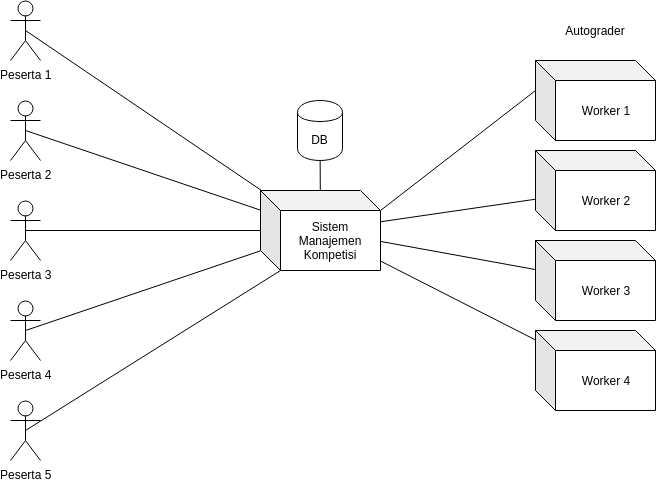
\includegraphics[width=0.7\textwidth]{images/architecture-old}
    \caption{Arsitektur Sistem \textit{Online Judge} Pada Saat Ini}
    \label{fig:architecture-old}
\end{figure}

\section{Sistem \textit{Autograder}} \label{subsec:autograder}

\par Sistem manajemen kompetisi memerlukan \textit{autograder} untuk menilai jawaban peserta kompetisi secara otomatis. Sistem \textit{online judge} yang sering digunakan saat ini menggunakan \textit{autograder} yang dipasang oleh juri pada beberapa komputer yang sudah disediakan oleh juri. Pada tugas akhir ini, diciptakan sistem \textit{autograder} yang dapat berjalan pada komputer peserta. Komputer peserta akan bertindak sebagai \textit{worker} yang menjalankan sistem \textit{autograder}. \textit{Worker} adalah komputer yang digunakan oleh sistem \textit{autograder} untuk melakukan kompilasi dan eksekusi terhadap jawaban peserta. Dalam tugas akhir ini, komputer peserta adalah \textit{worker} dari sistem \textit{autograder}. Terdapat beberapa aspek yang perlu diperhatikan dalam mengembangkan sistem \textit{autograder} seperti pengukuran waktu dan memori, \textit{load balancing}, evaluasi jawaban peserta, dan pengiriman \textit{test-case} ke \textit{worker}. Gambar \ref{fig:architecture-new} menggambarkan arsitektur sistem \textit{online judge} yang dibuat pada tugas akhir ini.

\begin{figure}[ht!]
    \centering
    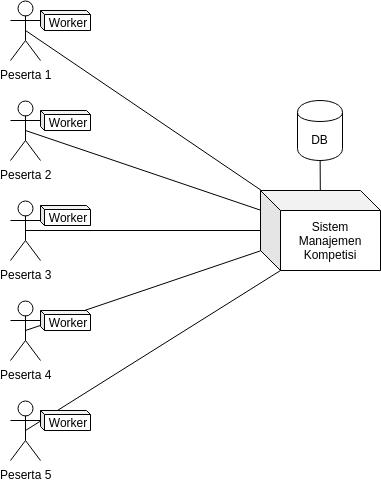
\includegraphics[width=0.5\textwidth]{images/architecture-new}
    \caption{Arsitektur Sistem \textit{Online Judge} Yang Dibuat}
    \label{fig:architecture-new}
\end{figure}

\subsection{Pengukuran Waktu Dan Memori} \label{subsec:time-memory-measure}

\par Komputer peserta memiliki spesifikasi yang berbeda-beda. Perbedaan spesifikasi tersebut menimbulkan beberapa perbedaan ketika sebuah program yang sama dieksekusi. Program yang sama dengan masukan yang sama dapat berjalan dengan waktu dan memori yang berbeda pada komputer yang berbeda. Komputer dengan \textit{clock-speed} yang lebih tinggi akan menjalankan program dengan lebih cepat. Komputer dengan \textit{core} yang lebih banyak juga akan menjalankan program parallel dengan lebih cepat. Selain itu, ukuran \textit{cache} dari komputer juga memengaruhi kecepatan waktu eksekusi. Kebutuhan memori dari suatu program juga ditentukan oleh spesifikasi komputer. Komputer dengan arsitektur 64-bit umumnya memerlukan memori yang lebih besar dibandingkan arsitektur 32-bit. Oleh karena itu, program yang dieksekusi pada komputer yang berbeda akan memerlukan waktu dan memori yang berbeda pula.

\par Penilaian jawaban peserta memerlukan metode pengukuran waktu dan memori yang adil sehingga program peserta yang benar akan dianggap benar oleh setiap \textit{worker}. Begitu juga program peserta yang salah akan dianggap salah oleh setiap \textit{worker}. Pada bab ini, dipaparkan beberapa teknik yang dapat digunakan untuk mengukur waktu eksekusi jawaban peserta.

\subsubsection{Spesifikasi CPU dan Sistem Operasi}

\par Kecepatan eksekusi sebuah program bergantung pada \textit{clock-speed} dan ukuran \textit{cache} dari CPU. Jika suatu proses hanya diberikan satu buah \textit{core} dari CPU, maka jumlah \textit{core} dari CPU dapat dianggap tidak memengaruhi kecepatan eksekusi proses tersebut. Kecepatan eksekusi program dapat diukur berdasarkan spesifikasi CPU dari komputer yang menjalankannya. Program yang dijalankan pada komputer dengan \textit{clock-speed} dan ukuran \textit{cache} yang rendah akan diberikan batasan waktu yang lebih lama. Sedangkan program yang dijalankan pada komputer dengan \textit{clock-speed} dan ukuran \textit{cache} yang lebih tinggi akan diberikan batasan waktu yang lebih singkat. Kebutuhan memori dari program yang dijalankan pada suatu komputer dipengaruhi oleh arsitektur komputer tersebut. Komputer peserta dapat memiliki arsitektur yang berbeda-beda. Komputer dengan arsitektur 64-bit umumnya memerlukan memori yang lebih besar dibandingkan dengan komputer dengan arsitektur 32-bit. Dengan mengetahui arsitektur komputer, kebutuhan memori dari suatu program dapat diperkirakan.

\par Pada penilaian jawaban peserta, diperlukan pengukuran waktu dan memori yang sangat akurat. Pengukuran waktu atau memori yang tidak akurat akan menimbulkan ketidakadilan dalam melakukan penilaian jawabab peserta. Dengan hanya memerhatikan spesifikasi dari CPU dan sistem operasi pada komputer peserta, pengukuran waktu dan memori yang akurat sulit dilakukan. Program yang berjalan pada sistem operasi 64-bit tidak selalu memerlukan memori dua kali dari program yang berjalan pada sistem operasi 32-bit. Kebutuhan memori bergantung pada isi dari program yang dijalankan dan beberapa faktor lain. Kecepatan eksekusi dari suatu program pun bergantung dari beberapa faktor lain sehingga pengukuran waktu dengan cara ini sulit untuk dilakukan.

\subsubsection{CPU \textit{Benchmarking}}

\par \textit{Benchmarking} dapat dilakukan untuk mengukur kinerja CPU dengan menggunakan sebuah program \textit{test}. Program \textit{test} dapat dijalankan pada CPU untuk mengukur waktu eksekusinya. Program \textit{test} yang dijalankan pada komputer pengguna akan dicatat jumlah instruksi dan waktunya. Jumlah instruksi dan waktu yang dibutuhkan untuk menjalankan program \textit{test} dapat digunakan untuk mengukur kinerja CPU. Batas waktu dari jawaban peserta kemudian ditentukan berdasarkan hasil eksekusi program \textit{test} tersebut.

\par \textit{Benchmarking} pada komputer peserta memiliki celah keamanan. Peserta bisa saja menjalankan program yang berat ketika proses \textit{benchmarking} dilakukan. Hal ini akan menyebabkan waktu eksekusi menjadi lambat dan dapat meningkatkan batasan waktu dari jawaban peserta.

\par Selain adanya celah keamanan, terdapat kesulitan lain yang ditemukan ketika melakukan \textit{benchmarking} yaitu pembuatan program \textit{test}. Program \textit{test} perlu dibuat sedemikian rupa sehingga dapat memberikan pengukuran waktu dan memori yang akurat. Untuk mengukur waktu eksekusi dan penggunaan memori dari program peserta dengan kompleksitas yang berbeda, diperlukan program \textit{test} yang berbeda. Hal ini mengakibatkan perlunya membuat program \textit{test} untuk setiap jenis soal yang ada pada kompetisi \textit{competitive programming}. Pembuatan program \textit{test} ini kemudian memberatkan juri karena juri perlu memikirkan program \textit{test} yang cocok sehingga dapat memberikan pengukuran waktu dan memori yang akurat.

\subsubsection{\textit{Benchmarking} Dengan Solusi Juri} \label{subsec:time-memory-measure-compare-with-jury}

\par Teknik \textit{benchmarking} sebenarnya efektif digunakan oleh \textit{autograder} untuk melakukan pengukuran waktu. Meskipun begitu, teknik \textit{benchmarking} tidak efisien dan memiliki celah keamanan jika digunakan. Juri perlu membuat sebuah program \textit{test} untuk setiap soal yang diberikan kepada peserta. Hal ini memberatkan pekerjaan juri sehingga dinilai tidak efisien. Selain itu, peserta dapat menjalankan proses yang berat pada komputernya sehingga memengaruhi keakuratan teknik \textit{benchmarking}.

\par Terdapat teknik yang dapat digunakan untuk meningkatkan efisiensi teknik \textit{benchmarking}. Teknik \textit{benchmarking} dapat menjadi lebih efisien dengan menghindari pembuatan program \textit{test} dari setiap soal pada kompetisi \textit{competitive programming}. Setiap soal dari kompetisi \textit{competitive programming} memiliki solusi yang telah dibuat juri. Solusi dari juri tersebut dapat digunakan sebagai program \textit{test}. Solusi \textit{juri} memiliki kompleksitas yang sesuai dengan soal yang telah dibuat oleh juri sehingga dapat menjadi program \textit{test} yang dapat digunakan untuk mengukur waktu eksekusi dan penggunaan memori dari program peserta secara akurat. Dengan menggunakan solusi juri sebagai program \textit{test}, juri tidak perlu membuat program \textit{test} khusus sehingga proses \textit{benchmarking} dapat menjadi lebih efisien.

\par Selain masalah efisiensi, teknik \textit{benchmarking} juga memiliki permasalahan lain yaitu bagaimana menghindari kecurangan peserta. Peserta bisa saja menjalankan proses yang berat pada komputernya sehingga mengganggu keakuratan proses \textit{benchmarking}. Hal ini menyebabkan sistem \textit{autograder} menganggap bahwa komputer peserta merupakan komputer yang lambat dan mengakibatkan jawaban peserta yang lambat bisa jadi dianggap jawaban yang benar.

\par Terdapat teknik yang dapat digunakan untuk menghindari kecurangan peserta pada paragraf sebelumnya. Pengukuran waktu yang dilakukan pada saat benchmarking dapat dilakukan dengan hanya memperhitungkan \textit{CPU Time}. \textit{CPU Time} merupakan waktu dimana proses sedang dijadwalkan untuk dieksekusi oleh \textit{CPU}. Ketika peserta menjalankan banyak proses yang berat, maka \textit{CPU} akan dijadwalkan untuk mengeksekusi proses yang terkait dengan \textit{autograder} secara lebih jarang. Hal ini dikarenakan sistem operasi membagikan \textit{CPU} secara adil untuk seluruh proses yang ada. Dengan cara ini, waktu yang dijadwalkan untuk proses lain tidak akan dihitung dalam \textit{benchmarking}.

\par Sistem operasi berbasis Linux menyediakan fitur \textit{cgroup} yang dapat digunakan untuk melakukan pengukuran \textit{CPU Time} dari suatu proses. Dengan menggunakan \textit{cgroup}, \textit{resource} yang digunakan oleh proses dapat dipantau. \textit{Cgroup} memungkinkan suatu proses untuk memantau penggunaan CPU dan memori dari proses lain. 

\begin{figure}[ht!]
    \centering
    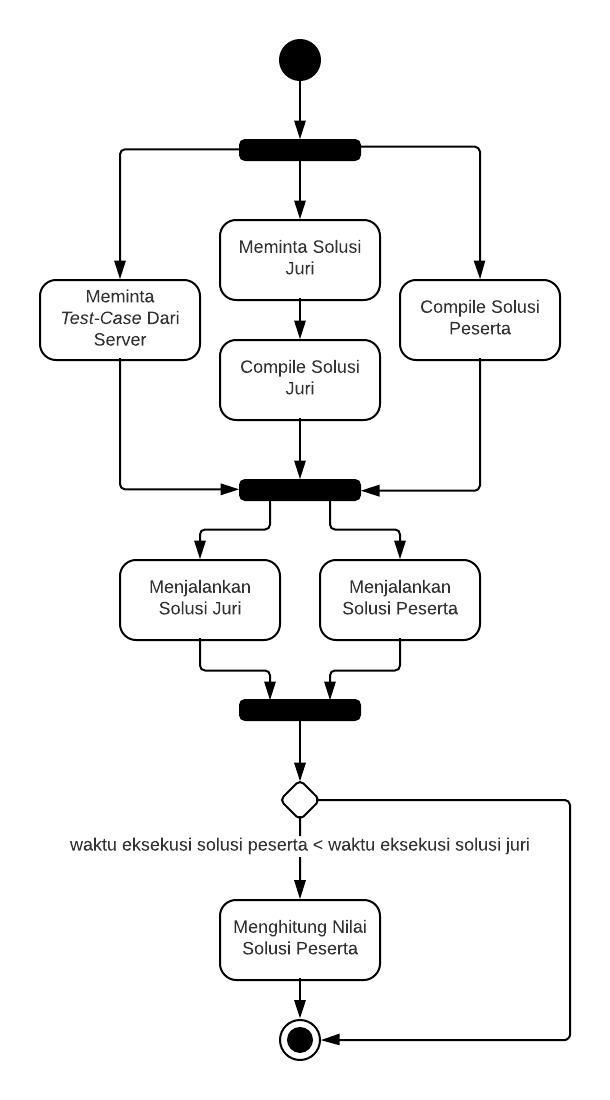
\includegraphics[width=0.5\textwidth]{images/cpu-time-counting}
    \caption{Diagram Aktivitas Penilaian Solusi Peserta}
    \label{fig:cpu-time-counting}
\end{figure}

\par \textit{Autograder} perlu menentukan apakah solusi peserta masih berada pada batas waktu yang diinginkan oleh juri. Hal tersebut dapat dicapai dengan membandingkan waktu eksekusi solusi peserta dengan waktu eksekusi solusi juri. Jika waktu eksekusi solusi peserta masih lebih cepat dari waktu eksekusi solusi juri, maka solusi peserta akan dianggap memenuhi batas waktu.

\par Meskipun solusi juri dan solusi peserta dieksekusi pada komputer yang sama. Waktu eksekusi kedua program tersebut dapat sedikit berbeda karena adanya perbedaan implementasi antara solusi peserta dan juri. Solusi peserta bisa saja lebih lambat atau lebih cepat dibandingkan dengan solusi juri. Untuk mengatasi perbedaan waktu ini, sebuah faktor toleransi dapat diterapkan pada sistem \textit{autograder}. Solusi peserta dapat diterima jika waktu eksekusinya masih berada pada batas toleransi dari solusi juri. Secara matematis, solusi peserta akan diterima jika memenuhi persamaan berikut $ T_{peserta} < (1 + \gamma) \times T_{juri}$, dengan $\gamma$ adalah nilai dari faktor toleransi.

\par Dengan membandingkan penggunaan CPU dan memori dari solusi peserta dengan solusi juri, perhitungan waktu dan memori yang akurat dapat dilakukan. Meskipun peserta menjalankan program yang berat pada saat penilaian dilakukan, perbandingan waktu eksekusi dari program solusi juri dengan program solusi peserta akan tetap sama. Oleh karena itu, teknik ini digunakan untuk melakukan pengukuran waktu dan memori dalam menyelesaikan tugas akhir ini. Gambar \ref{fig:cpu-time-counting} menjelaskan proses penilaian jawaban peserta dengan membandingkan dengan program solusi juri. 

\lstinputlisting[caption={Contoh Program yang \textit{IO bound}},label={lst:busysleeping},language=C,style=CStyle]{listings/busy-sleep.c}

\par Dengan hanya menghitung \textit{CPU Time} dari proses, terdapat masalah lain yang muncul. Peserta bisa saja mengirimkan jawaban berupa program yang bersifat \textit{IO bound}. Program yang bersifat \textit{IO bound} tidak menggunakan banyak \textit{CPU Time}. Kode \ref{lst:busysleeping} merupakan contoh program yang bersifat \textit{IO bound}. Program tersebut tidak menggunakan banyak \textit{CPU Time} karena hanya melakukan \textit{sleep}. Pada saat \textit{sleep}, proses yang berjalan tidak akan dijadwalkan untuk dieksekusi oleh \textit{CPU}. Hal tersebut menyebabkan proses dapat berjalan dengan sangat lama akan tetapi \textit{CPU Time}-nya bernilai hampir nol. Program tersebut akan mengakibatkan \textit{autograder} tidak pernah selesai melakukan pengukuran waktu karena \textit{CPU Time}-nya sangat kecil dan proses tidak pernah selesai untuk dijalankan.

\par Untuk mengatasi proses yang bersifat \textit{IO bound}, waktu eksekusi dapat dibatasi oleh \textit{wall-clock time}. \textit{Wall-clock} merupakan waktu sebenarnya dimana proses berada berada dalam sistem operasi komputer. Proses yang berjalan ketika melakukan \textit{benchmarking} dapat dibatasi \textit{Wall-clock time}-nya. Batas \textit{wall-clock time} dapat diatur sedemikian rupa sehingga dapat dipastikan bahwa solusi peserta yang melewati batas ini dipastikan tidak lolos. Salah satu contoh batas \textit{wall-clock time} adalah satu detik ditambah lamanya \textit{CPU time} dari proses eksekusi solusi juri.

\par Penentuan batas \textit{wall-clock time} sulit dilakukan pada komputer dengan spesifikasi yang berbeda-beda. Komputer yang berbeda mungkin memiliki kecepatan \textit{IO} yang berbeda. Hal ini mengakibatkan juri perlu memerhatikan spesifikasi setiap komputer peserta untuk mengatur nilai \textit{wall-clock time} yang tepat. Selain itu, setiap proses pada sistem operasi yang berbasis Linux memiliki prioritas yang dapat diatur. Peserta bisa saja menjadikan sistem \textit{autograder} memiliki prioritas rendah sehingga proses yang melakukan pengukuran waktu jarang dijadwalkan oleh sistem operasi. Hal tersebut mengakibatkan berkurangnya keakuratan proses \textit{benchmarking}.

\par Untuk mengatasi permasalahan pada paragraf di atas, kecepatan \textit{IO} dari setiap komputer peserta yang digunakan untuk pengukuran waktu dapat dibatasi sehingga seluruh komputer peserta memiliki kecepatan \textit{IO} yang sama. Selain itu, proses \textit{autograder} dapat diatur untuk memiliki prioritas yang tinggi sehingga lebih sering dijadwalkan oleh sistem operasi. Pada tugas akhir ini solusi tersebut tidak digunakan karena masih perlu adanya penelitian lebih lanjut. Pada tugas akhir ini, ketika pengukuran waktu sudah melebihi batas \textit{wall-clock time}, \textit{autograder} akan memberikan \textit{verdict} \textit{Internal Error} yang menandakan proses penilaian gagal. Penilaian yang gagal tidak akan dihitung dan akan dijadwalkan untuk dikerjakan oleh komputer peserta lain. 

\subsection{\textit{Load Balancing}}

\begin{figure}[ht!]
    \centering
    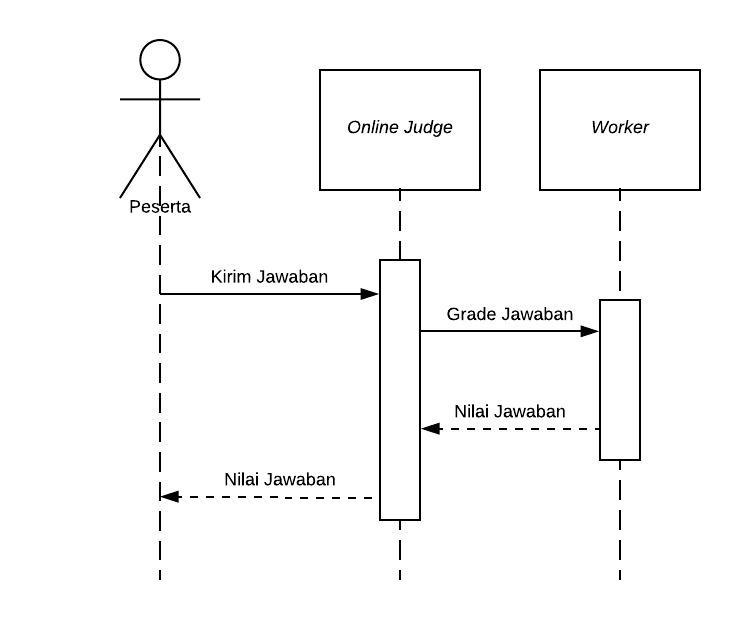
\includegraphics[width=0.75\textwidth]{images/load-balancing-push}
    \caption{\textit{Push-Based Load Balancer}}
    \label{fig:load-balancing-push}
\end{figure}

\par Dalam membangun sistem \textit{autograder}, diperlukan pembagian kerja kepada \textit{worker-worker} yang ada. \textit{Worker} yang dimaksud adalah komputer yang bekerja melakukan penilaian jawaban peserta. Dalam tugas akhir ini, \textit{worker} merupakan komputer peserta. Karena spesifikasi komputer tiap \textit{worker} berbeda-beda, diperlukan teknik pembagian kerja yang adil kepada seluruh seluruh \textit{worker}. Selain itu, aspek keamanan juga perlu diperhatikan karena jawaban peserta akan dikirimkan ke \textit{worker} lain. Terdapat beberapa pendekatan pembagian kerja yang dapat digunakan, yaitu: \textit{push-based}, \textit{pull-based}, dan \textit{self-grading}.

\par Pada pendekatan \textit{push-based}, sistem \textit{autograder} memerlukan sebuah \textit{master} yang akan membagikan pekerjaan ke seluruh \textit{worker}. \textit{Master} akan menentukan \textit{worker} mana yang akan diberikan suatu pekerjaan. Dengan menggunakan metode ini, \textit{master} perlu mengetahui informasi \textit{resource} dari seluruh \textit{worker} yang ada. Setiap \textit{worker} perlu mengirimkan informasi \textit{resource}-nya kepada \textit{master}. Metode ini cukup sulit untuk dilakukan karena perlunya mengimplementasikan algoritma \textit{load balancing} pada \textit{master}. Gambar \ref{fig:load-balancing-push} menggambarkan alur pembagian kerja dengan metode \textit{push-based}.

\begin{figure}[ht!]
    \centering
    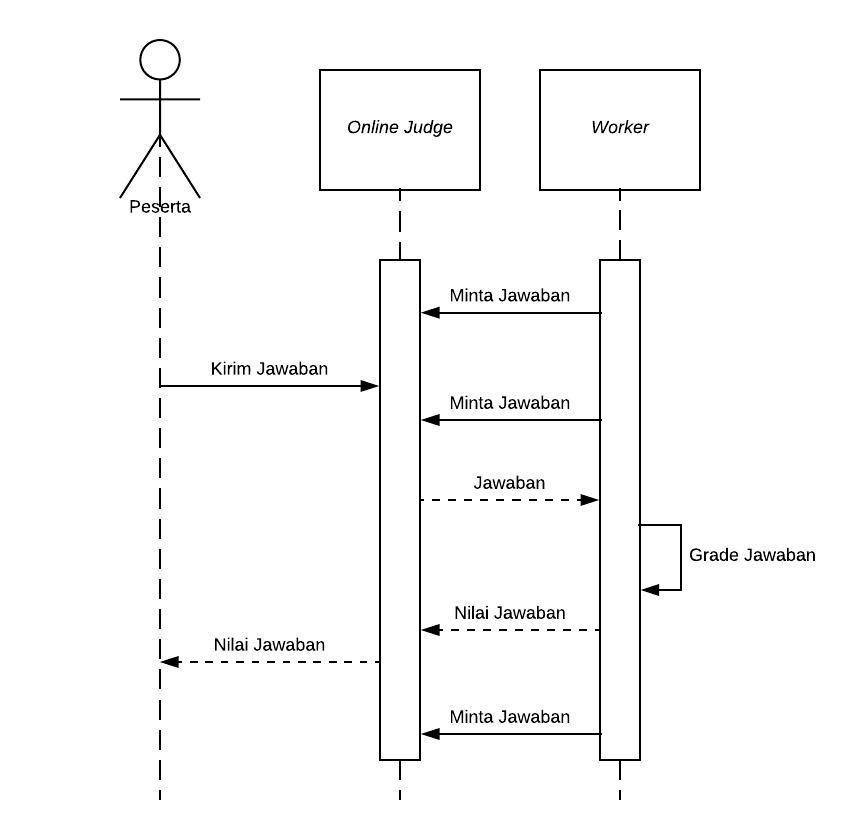
\includegraphics[width=0.75\textwidth]{images/load-balancing-pull}
    \caption{\textit{Pull-Based Load Balancer}}
    \label{fig:load-balancing-pull}
\end{figure}

\par Pada pendekatan \textit{pull-based}, diperlukan juga sebuah \textit{master} yang akan menyimpan seluruh pekerjaan yang perlu diselesaikan. Pendekatan \textit{pull-based} berbeda dengan pendekatan \textit{push-based} dimana \textit{master} lah yang memberikan pekerjaan kepada \textit{worker}. Pada pendekatan \textit{pull-based}, \textit{worker} yang sedang tersedia akan meminta pekerjaan kepada \textit{master}. Dengan pendekatan ini, pembagian pekerjaan akan menjadi rata dengan sendirinya. Metode ini lebih mudah untuk diimplementasikan dibanding dengan metode \textit{push-bashed} karena tidak perlu membuat algoritma \textit{load balancing} yang spesifik pada \textit{master}. Gambar \ref{fig:load-balancing-pull} menggambarkan alur pembagian kerja dengan metode \textit{pull-based}.

\par Selain pendekatan \textit{push-based} dan \textit{pull-based}, terdapat pendekatan lain yang lebih sederhana yaitu \textit{self-grading}. Pada \textit{self-grading}, peserta akan menilai jawabannya sendiri. Dengan menggunakan pendekatan ini, tidak diperlukan adanya \textit{master}. Meskipun begitu, pendekatan \textit{self-grading} memiliki celah keamanan karena peserta mengetahui jawaban siapa yang dinilai pada komputernya. Hal ini memungkinkan peserta untuk melakukan serangan-serangan yang mengakibatkan jawaban yang dinilai pada komputernya selalu dianggap benar.

\par Pendekatan \textit{pull-based} lebih adil dan lebih mudah diimplementasikan dibandingkan dengan pendekatan \textit{push-based}. Pendekatan \textit{pull-based} lebih aman dibandingkan dengan pendekatan \textit{self-grading} karena identitas jawaban yang dinilai pada \textit{worker} lebih rahasia. Oleh karena itu, pendekatan \textit{pull-based load balancing} digunakan pada tugas akhir ini karena lebih adil dan lebih aman dibandingkan dengan dua pendekatan lainnya.

\par Untuk meningkatkan keamanan, jawaban peserta dapat dinilai pada lebih dari satu buah \textit{worker}. Jawaban peserta dinilai benar jika mayoritas dari \textit{worker} yang menilai jawaban peserta tersebut menyatakan bahwa jawaban tersebut adalah benar. Dengan menilai jawaban peserta di banyak \textit{worker}, risiko yang timbul sebab adanya kecurangan yang dilakukan peserta dapat berkurang. Pada tugas akhir ini, \textit{load balancing} dilakukan dengan pendekatan \textit{pull-based} dan dengan melakukan penilaian jawaban peserta pada lebih dari satu buah \textit{worker}.

\subsection{Evaluasi Jawaban Menggunakan Sandbox}

\par Dalam melakukan penilaian terhadap jawaban peserta, diperlukan adanya proses kompilasi dan eksekusi terhadap program yang dikirimkan peserta. Proses kompilasi dan eksekusi ini akan dijalankan pada \textit{worker}. Proses ini dapat membahayakan lingkungan \textit{worker} jika peserta mengirimkan kode program yang berbahaya. Untuk menghindari kerusakan pada \textit{worker}, proses ini perlu diisolasi sehingga tidak berpengaruh pada lingkungan \textit{worker}. Teknik untuk mengisolasi proses eksekusi program ini dinamakan \textit{sandboxing}. Terdapat beberapa teknik \textit{sandboxing} yang dapat digunakan seperti \textit{virtual machine} dan \textit{containerization}.

\subsubsection{Menggunakan \textit{Virtual Machine}}

\par \textit{Virtual machine} memberikan isolasi kepada program pada tingkat \textit{hardware}. Komputer yang ada pada saat ini memiliki \textit{hypervisor} yang dapat digunakan untuk menyimulasikan \textit{hardware} dari komputer. Dengan menggunakan \textit{virtual machine}, komputer dapat menjalankan sistem operasi virtual di atas sistem operasi yang sedang berjalan. \textit{Virtual machine} memberikan layanan isolasi yang sangat aman.

\par Meskipun keamanan \textit{virtual machine} sangat tinggi, akan tetapi banyak \textit{overhead} yang ditimbulkan. Untuk menyalakan \textit{virtual machine}, membutuhkan waktu yang lama dan memori yang cukup besar. Selain itu, diperlukan adanya sistem operasi baru yang berjalan di atas \textit{virtual machine} yang dibuat. Hal ini menyebabkan proses penilaian jawaban peserta menjadi lambat dan membutuhkan sangat banyak memori.

\subsubsection{Menggunakan \textit{Container}}

\par \textit{Container} merupakan suatu teknik untuk mengisolasi proses pada tingkat \textit{software}. Dengan menggunakan \textit{container}, proses yang berjalan pada sistem operasi berbasis Linux dapat dibatasi \textit{resource}-nya. Penggunaan memori dan CPU dari suatu proses dapat dibatasi sehingga tidak membebani komputer peserta. Selain itu, Linux memiliki fitur yang memungkinkan pengguna mengisolasi suatu proses sehingga proses tersebut tidak dapat mengatahui informasi rahasia yang ada pada komputer peserta. \textit{Container} dapat dibuat dengan memanfaatkan fitur dari sistem operasi berbasis Linux yaitu: \textit{chroot}, \textit{namespace}, \textit{rlimit} dan \textit{cgroup}. Pada tugas akhir ini, \textit{container} digunakan untuk melakukan isolasi pada proses yang berjalan pada komputer peserta. Teknik ini dipilih karena memberikan isolasi yang cukup, dan tidak menimbulkan \textit{overhead} yang sangat besar seperti teknik isolasi dengan \textit{virtual machine}.

\par \textit{Chroot} memungkinkan proses pada sistem operasi berbasis Linux untuk memiliki \textit{filesystem} sendiri. Hal ini dapat dilakukan dengan mengganti \textit{root} dari proses ke \textit{directory} tertentu. Dengan mengganti \textit{root}, maka proses tidak dapat mengakses \textit{file} yang berada di luar \textit{directory root}. \textit{Chroot} dapat dilakukan dengan melakukan pemanggilan \textit{system call chroot}. \textit{System call chroot} hanya dapat dilakukan oleh proses yang memiliki akses \textit{root} atau memiliki \textit{capability} \textit{CAP\_SYS\_CHROOT}. Pada tugas akhir ini, program \textit{autograder} diberikan akses \textit{root} sehingga dapat melakukan pemanggilan \textit{system call chroot}.

\par \textit{Namespace} merupakan fitur dari Linux yang memungkinkan pengisolasian suatu proses sehingga tidak mengetahui informasi lain di luar \textit{namespace}-nya. Setiap proses pada Linux memiliki \textit{namespace}. Proses yang berada pada \textit{namespace} tidak akan mengetahui informasi dari \textit{namespace} lain. Hal ini memungkinkan suatu proses untuk diisolasi sehingga tidak mengatahui adanya proses lain, \textit{user} lain, ataupun \textit{network interface} lain. Dengan menggunakan \textit{namespace}, keamanan dari lingkungan \textit{worker} dapat dijaga karena jawaban peserta tidak mengetahui informasi mengenai komputer peserta. Pada tugas akhir ini, proses evaluasi jawaban peserta dilakukan di dalam \textit{namespace} yang terpisah dari \textit{namespace} pengguna.

\par Setiap proses pada sistem operasi berbasis Linux memiliki batas \textit{resource} yang dapat digunakan. Batas tersebut dapat diatur dengan melakukan pemanggilan \textit{system call setrlimit}. Proses yang menggunakan \textit{resource} melebihi batas akan dihentikan oleh sistem operasi. Pada tugas akhir ini, \textit{system call setrlimit} digunakan untuk membatasi jumlah proses yang dapat diciptakan, jumlah \textit{open file descriptor} yang dapat dimiliki, dan ukuran file yang dapat diciptakan oleh program peserta.

\par \textit{Cgroup} merupakan fitur dari sistem operasi berbasis Linux yang dapat digunakan untuk membatasi penggunaan \textit{resource} suatu proses. Selain itu, \textit{cgroup} juga dapat digunakan untuk memantau penggunaan \textit{resource} dari proses tersebut. Pada tugas akhir ini, \textit{cgroup} digunakan untuk mengukur penggunaan CPU dan memori dari proses yang berjalan dan menghentikan proses yang menggunakan \textit{resource} secara berlebihan.

\subsection{Kompilasi Program}

\par Penilaian terhadap jawaban peserta memerlukan adanya tahap kompilasi agar program dapat dijalankan. Keamanan dari proses kompilasi tentunya juga perlu dijaga. Keamanan dari proses kompilasi dapat dicapai dengan menggunakan \textit{sandbox} seperti yang sudah dijelaskan pada subbab sebelumnya.

\par Salah satu aspek yang perlu diperhatikan dalam melakukan kompilasi adalah pengadaan \textit{compiler}. \textit{Compiler} merupakan program yang digunakan untuk melakukan kompilasi kode sumber menjadi program yang dapat dijalankan pada sistem operasi. Komputer peserta tentunya perlu memiliki \textit{compiler} untuk melakukan kompilasi. Untuk menjaga keadilan, seluruh \textit{compiler} yang ada pada komputer peserta perlu memiliki versi yang sama. \textit{Compiler} dengan versi yang berbeda dapat menghasilkan program dengan kemampuan yang berbeda. Terkadang \textit{compiler} dengan versi yang lebih baru dapat memberikan optimisasi pada program sehingga berjalan dengan lebih cepat. Perbedaan versi \textit{compiler} pada komputer peserta akan memberikan ketidakadilan dalam proses penilaian.

\par Masalah pada paragraf sebelumnya diatasi dengan melengkapi \textit{autograder} dengan \textit{compiler}. Karena ukuran \textit{compiler} umumnya cukup besar, maka \textit{compiler} di-\textit{compress} ketika didistribusikan ke komputer peserta. Setiap sistem \textit{autograder} dijalankan, \textit{compiler} akan di-\textit{extract} sehingga siap digunakan.

\subsection{Pengiriman \textit{Test-Case} Ke \textit{Worker}} \label{subsec:sending-test-case-to-worker}

\par Dalam melakukan penilaian jawaban peserta perlu adanya pengiriman \textit{test-case} dari \textit{server} ke \textit{worker}. \textit{Test-case} merupakan informasi yang digunakan untuk menentukan kebenaran jawaban peserta sehingga informasi ini bersifat rahasia dan tidak boleh diketahui oleh peserta maupun orang lain di luar kompetisi. \textit{Test-case} digunakan sebagai masukan pada saat menjalankan program solusi peserta dan juri. Kebenaran dari solusi peserta dinilai dari keluaran yang dihasilkan. Salah satu cara untuk menilai kebenaran program peserta tersebut adalah dengan membandingkan keluaran program solusi peserta dengan keluaran program solusi juri. Jika keluaran solusi peserta sama seperti keluaran solusi juri, maka solusi peserta akan dianggap benar. Akan tetapi, seringkali keluaran dari program solusi peserta tidak harus sama persis dengan solusi juri. Soal pada \textit{competitive programming} seringkali memiliki lebih dari satu solusi yang sah dan tidak mungkin untuk menuliskan semua solusi satu per satu. Oleh karena itu, diperlukan juga adanya program \textit{checker} yang digunakan untuk menentukan kebenaran solusi peserta. Program \textit{checker} akan menilai kebenaran solusi peserta berdasarkan keluaran dari program solusi peserta dan program solusi juri.

\par \textit{Test-case} dan \textit{checker} merupakan informasi rahasia yang perlu dipertukarkan antara \textit{worker} dan \textit{server}. Pertukaran informasi rahasia ini dapat dilakukan dengan menggunakan teknik kriptografi dimana informasi akan dienkripsi terlebih dahulu sebelum dikirimkan. Proses enkripsi dan dekripsi dapat dilakukan pada lapisan \textit{transport} menggunakan TCP dengan TLS.

\begin{figure}[ht!]
    \centering
    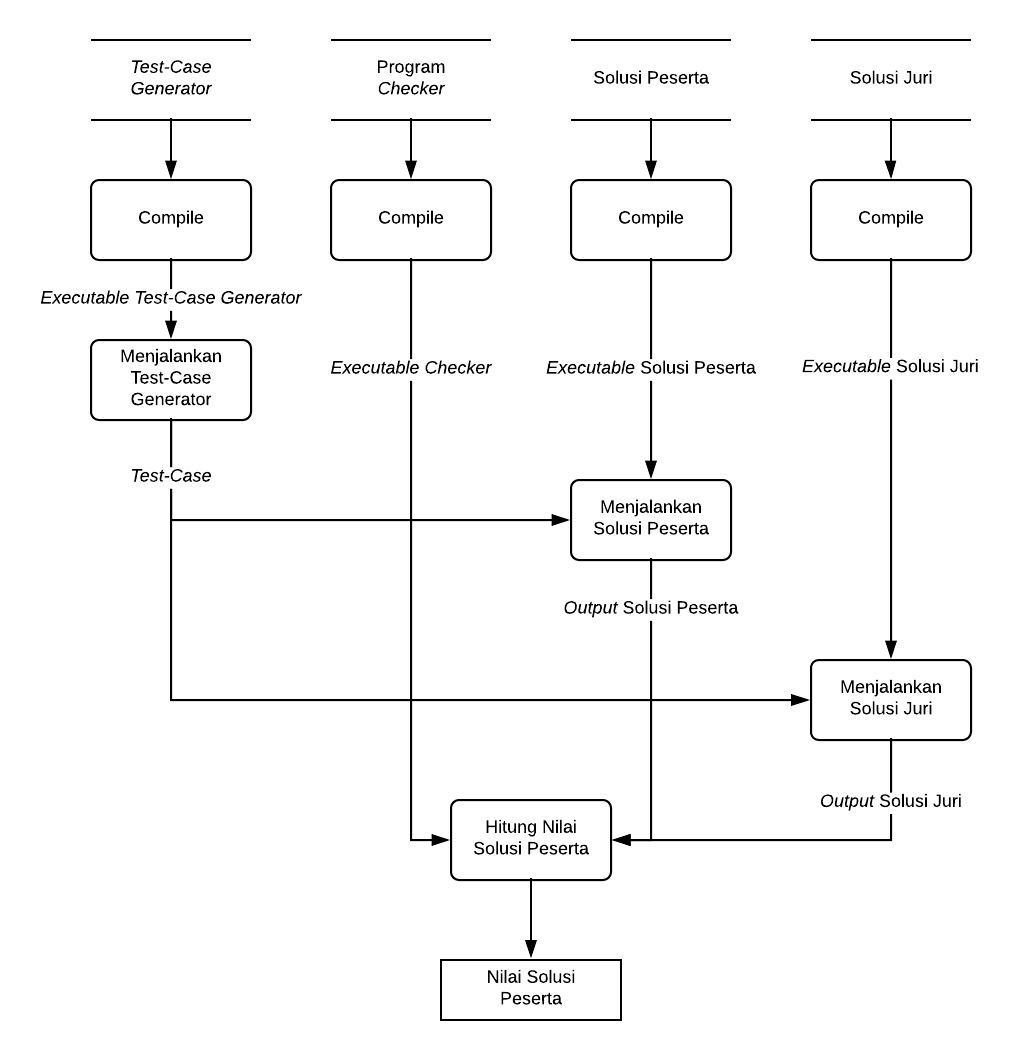
\includegraphics[width=0.85\textwidth]{images/grading-dfd}
    \caption{Diagram Aliran Data Pada Proses Penilaian Solusi Peserta}
    \label{fig:grading-dfd}
\end{figure}

\par Dengan menggunakan TCP dan TLS, kebocoran informasi yang dikirimkan melalui jaringan dapat dihindari sehingga tidak ada pihak ketiga yang dapat mengetahui isi dari informasi tersebut. Akan tetapi, karena informasi ini diterima oleh komputer peserta, peserta dapat dengan mudah mengetahui isi dari informasi tersebut. Oleh karena itu, diperlukan satu lapisan enkripsi lagi pada aplikasi yang berjalan pada komputer peserta.

\begin{figure}[ht!]
    \centering
    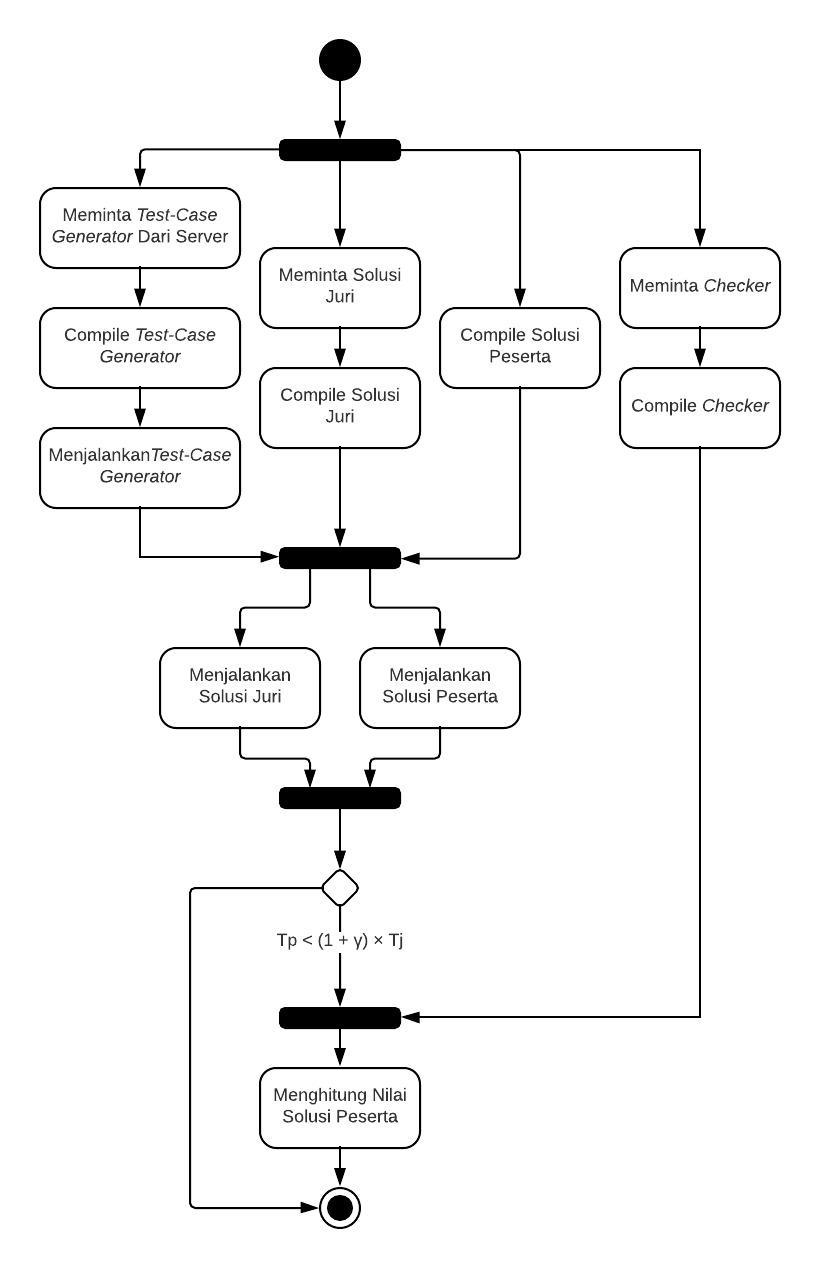
\includegraphics[width=0.65\textwidth]{images/total-grader-activity}
    \caption{Alur Proses Penilaian Jawaban Peserta}
    \label{fig:total-grader-activity}
\end{figure}

\par \textit{Test-case} umumnya merupakan file \textit{text} yang cukup besar. Pengiriman file ini dapat menghabiskan banyak \textit{bandwidth}. Meskipun begitu, \textit{test-case} biasanya dibuat dengan cara dibangkitkan oleh sebuah program yang dibuat oleh juri. \textit{Test-case} yang sama dapat dibangkitkan berulang-kali dengan menjalankan program tersebut. Untuk mengurangi kebutuhan \textit{bandwidth}, \textit{test-case} tidak perlu dikirim, melainkan program pembangkit \textit{test-case} saja yang dikirim. \textit{Test-case} yang akan digunakan untuk melakukan penilaian solusi peserta dibangkitkan dengan program pembangkit \textit{test-case} ini seperti pada Gambar \ref{fig:grading-dfd}. Diagram pada Gambar \ref{fig:total-grader-activity} menggambarkan alur proses penilaian jawaban peserta secara lengkap.

\par Pada tugas akhir ini, \textit{test-case} dipertukarkan dengan mengirimkan program pembangkit \textit{test-case} secara aman. Keamanan diperoleh dengan menggunakan dua kali enkripsi yaitu pada lapisan \textit{transport} dan aplikasi. Terdapat beberapa protokol yang dapat digunakan dalam melakukan pengiriman informasi ini. Protokol yang dipilih pada tugas akhir ini adalah protokol HTTP (\textit{hypertext transfer protocol}). Protokol ini dipilih karena aman dan mudah untuk digunakan.

\subsection{Menghadapi Serangan \textit{Reverse Engineering}}

\par Karena penilaian jawaban pada sistem \textit{online judge} yang dibangun dilakukan pada komputer peserta, maka muncul risiko adanya serangan \textit{reverse engineering} yang dapat dilakukan oleh pserta. Peserta dapat mengubah-ubah kode program dari \textit{autograder} yang dijalankan pada komputernya. Hal ini mengakibatkan peserta dapat mengubah kelakuan dari \textit{autograder}. Beberapa hal buruk yang mungkin terjadi antara lain adalah:
\begin{enumerate}
    \item Peserta dapat mengetahui kunci untuk melihat solusi juri dan \textit{testcase}.
    \item Peserta dapat selalu mengirimkan \textit{verdict} tertentu kepada sistem \textit{online judge}.
    \item Peserta dapat mengetahui jawaban dari peserta lain.
\end{enumerate}
Pada tugas akhir ini, diasumsikan peserta tidak melakukan serangan dalam bentuk \textit{reverse engineering}. Meskipun begitu, terdapat beberapa cara untuk mengurangi risiko yang muncul akibat serangan jenis ini.

\par Serangan \textit{reverse engineering} mungkin dilakukan oleh peserta jika peserta memiliki akses \textit{root} dari komputer yang digunakannya. Meskipun begitu, untuk beberapa jenis kompetisi \textit{competitive programming}, serangan ini dapat diatasi dengan tidak memberikan akses \textit{root} kepada peserta. Kompetisi ACM-ICPC merupakan salah satu jenis kompetisi yang dapat bertahan dari serangan \textit{reverse engineering}.

\par Pada kompetisi ACM-ICPC, peserta umumnya akan diseleksi terlebih dahulu secara bertingkat sebelum akhirnya berkompetisi di \textit{world final}. Sebelum babak \textit{world final}, jumlah peserta yang mengikuti kompetisi relatif sedikit sehingga sistem \textit{online judge} yang saat ini sering digunakan cukup untuk menjalankan kompetisi tersebut. Pada \textit{world final}, jumlah peserta kompetisi menjadi sangat banyak karena terdiri dari peserta-peserta yang lolos dari berbagai negara. Pada \textit{world final}, juri akan memberikan komputer khusus kepada peserta untuk mengikuti kompetisi tersebut. Pada babak \textit{world final}, juri dapat menggunakan komputer peserta sebagai \textit{worker} untuk menilai jawaban peserta. Juri dapat mengatur agar peserta tidak mendapatkan akses \textit{root} pada komputer yang digunakannya sehingga tidak dapat melakukan berbagai jenis serangan yang berupa \textit{reverse engineering}.

\par Untuk lebih mengurangi risiko yang muncul akibat serangan \textit{reverse engineering}, juri dapat mengatur agar setiap jawaban peserta dinilai oleh banyak \textit{worker}. Jika terdapat serangan \textit{reverse engineering} yang mengakibatkan \textit{worker} mengirimkan \textit{verdict} yang salah kepada \textit{server}, maka masih terdapat beberapa \textit{worker} lain yang mengirimkan \textit{verdict} yang benar. Peserta yang melakukan serangan \textit{reverse engineering} kemudian dapat dideteksi ketika \textit{verdict} yang dikirimkannya berbeda dengan peserta lain.

\par Sebagai contoh pada paragraf sebelumnya, misalkan setiap jawaban dinilai oleh lima buah \textit{worker}. Ketika sebuah jawaban dinilai, maka terdapat lima peserta berbeda yang melakukan penilain. Seorang peserta bisa saja melakukan serangan \textit{reverse engineering} dan mengakibatkan \textit{worker} pada komputernya mengirimkan \textit{verdict} yang salah kepada \textit{server}. Meskipun begitu, empat peserta lain yang tidak melakukan serangan \textit{reverse engineering} akan mengirimkan \textit{verdict} yang berbeda dengan peserta yang melakukan serangan \textit{reverse engineering}. Dengan mengamati kelima buah \textit{verdict} ini, peserta yang mengirimkan \textit{verdict} yang berbeda dapat dikatakan melakukan serangan.

% TODO: tambah cara penilaian, pikirin lagi tentang self-grading, tambah penjelasan satu jawaban bisa dinilai lebih dari satu kali, jelasin grading_size

\section{Sistem Manajemen Kompetisi}

\begin{figure}[ht!]
    \centering
    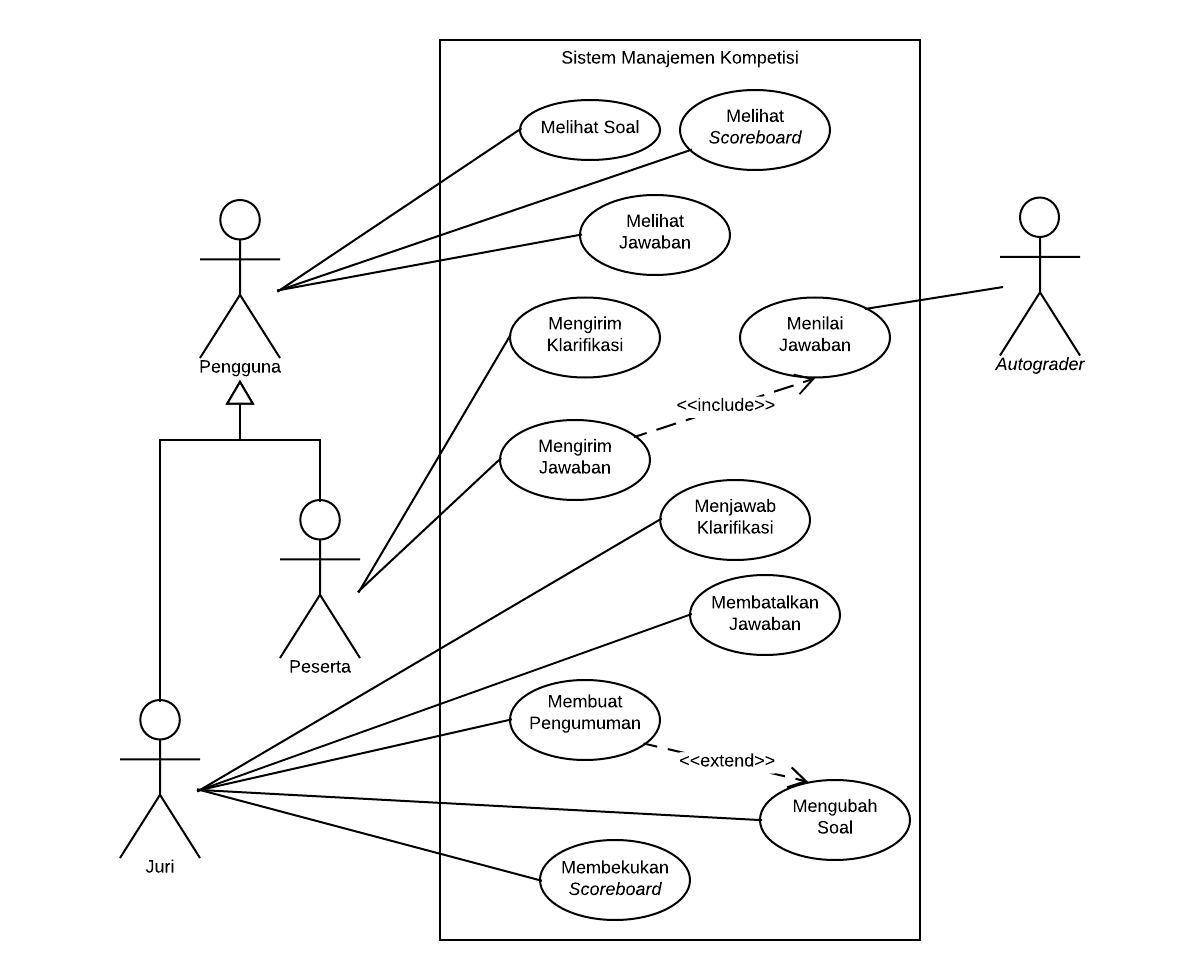
\includegraphics[width=0.85\textwidth]{images/oj-use-case}
    \caption{Diagram \textit{Use Case} Dari Sistem Manajemen Kompetisi}
    \label{fig:oj-use-case}
\end{figure}

\par Sistem manajemen kompetisi memberikan layanan kepada peserta kompetisi dan juri untuk berinteraksi. \textit{Online judge} yang populer pada saat ini memberikan sistem manajemen kompetisi berbasis \textit{web}. Sistem manajemen kompetisi ini dibutuhkan oleh peserta dan juri untuk melakukan aksi-aksi terkait kompetisi yang sedang berlangsung. Kebutuhan dari sistem manajemen kompetisi digambarkan oleh diagram \textit{use case} pada Gambar \ref{fig:oj-use-case}. Berikut ini adalah kebutuhan dari sistem manajemen kompetisi pada \textit{online judge}:

\begin{enumerate}
    \item Peserta dan juri dapat melihat soal.
    \item Peserta dapat mengirim jawaban.
    \item Sistem \textit{autograder} dapat menilai jawaban peserta.
    \item Peserta dapat mengirim klarifikasi soal.
    \item Juri dapat membuat pengumuman terkait kompetisi.
    \item Juri dapat menjawab klarifikasi peserta.
    \item Juri dapat mengubah soal.
    \item Peserta dan juri dapat melihat \textit{scoreboard}.
    \item Juri dapat membekukan \textit{scoreboard}.
    \item Peserta dapat melihat jawaban yang dikirim olehnya.
    \item Juri dapat melihat jawaban yang dikirim seluruh peserta.
    \item Juri dapat mengatur jawaban peserta untuk tidak dinilai.
\end{enumerate}

\par Pada tugas akhir ini, tidak semua kebutuhan dari sistem manajemen kompetisi diimplementasikan. Masalah yang ingin diselesaikan dalam tugas akhir ini tidak terletak pada sistem manajemen kompetisi, melainkan pada sistem \textit{autograder}. Oleh karena itu hanya kebutuhan yang berkaitan dengan proses penilaian saja yang diimplementasikan pada tugas akhir ini. Kebutuhan sistem manajemen kompetisi yang diimplementasikan pada tugas akhir ini antara lain adalah:

\begin{enumerate}
    \item Peserta dan juri dapat melihat soal.
    \item Peserta dapat mengirim jawaban.
    \item Sistem \textit{autograder} dapat menilai jawaban peserta.
    \item Juri dapat mengubah soal.
    \item Peserta dapat melihat jawaban yang dikirim olehnya.
    \item Juri dapat melihat jawaban yang dikirim seluruh peserta.
\end{enumerate}

\begin{figure}[ht!]
    \centering
    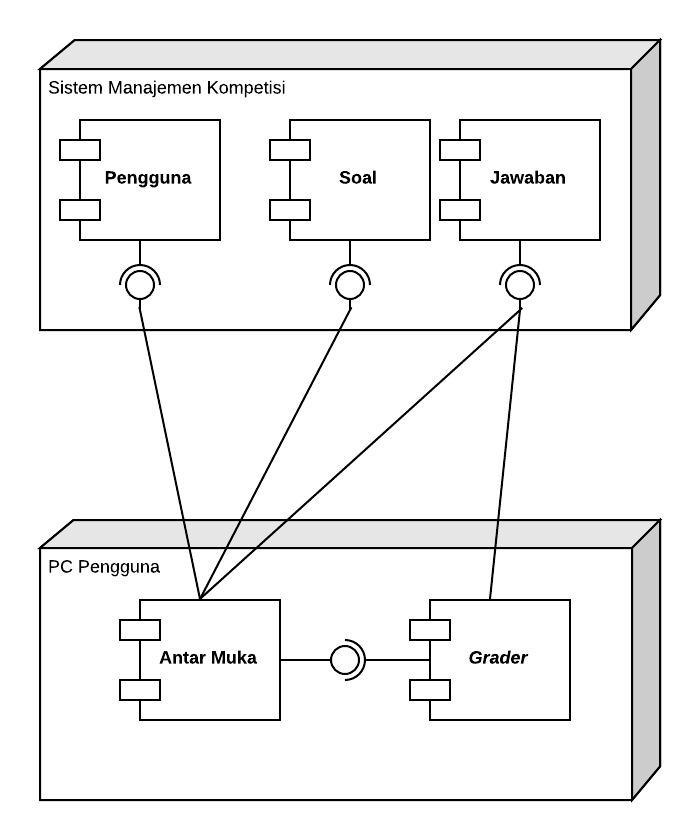
\includegraphics[width=0.5\textwidth]{images/oj-components}
    \caption{Diagram Komponen Sistem Manajemen Kompetisi}
    \label{fig:oj-components}
\end{figure}
% TODO: tambah komponen "kontes"

\par Sistem manajemen kompetisi yang digunakan pada tugas akhir ini mengikuti sistem manajemen kompetisi yang saat ini banyak digunakan. Sistem manajemen kompetisi ini dapat dibagi menjadi beberapa komponen utama yaitu: pengguna, soal, jawaban, antar muka dan \textit{grader}. Komponen \textit{grader} tidak lain adalah sistem \textit{autograder} yang telah dipaparkan pada bagian \ref{subsec:autograder}. Diagram komponen pada Gambar \ref{fig:oj-components} menggambarkan komponen yang digunakan dalam sistem manajemen kompetisi beserta keterhubungannya.

\subsection{Komponen Pengguna}

\par Kompetisi \textit{competitive programming} ada yang bersifat tertutup dimana hanya peserta tertentu yang dapat mengikutinya dan terbuka dimana setiap orang dapat mengikutinya. Sistem \textit{online judge} yang populer saat ini umumnya dapat menangani kedua jenis kompetisi tersebut. Untuk memasuki kompetisi, peserta perlu membuat akun di sistem \textit{online judge} tersebut terlebih dahulu. Peserta kemudian dapat memasuki kompetisi dengan cara melakukan \textit{login} pada sistem tersebut. Untuk menangani pendaftaran peserta baru dan \textit{login}, sistem \textit{online judge} perlu memiliki komponen manajemen pengguna yang bertugas melakukan otentikasi dan otorisasi pengguna. Beberapa \textit{online judge} memiliki komponen manajemen pengguna yang memanfaatkan layanan otentikasi dan otorisasi dari pihak ketiga seperti Google, Facebook, Github, dan Auth0. Terdapat juga sistem \textit{online judge} yang melakukan otentikasi dan otorisasi tanpa menggunakan pihak ketiga, misalnya DomJudge dan Mooshak.

\par Komponen pengguna dibuat pada sistem manajemen kompetisi untuk melakukan otentikasi dan otorisasi pengguna. Untuk menyederhanakan persoalan, pada tugas akhir ini komponen pengguna yang bertugas melakukan otentikasi dan otorisasi pengguna tidak akan menggunakan layanan pihak ketiga. Beberapa \textit{software development framework} seperti Django, Express, dan Laravel memiliki kemampuan untuk menangani masalah ini dengan mudah. Informasi pengguna akan disimpan pada sistem basis data yang sudah tersedia. Otentikasi pengguna akan dilakukan dengan sederhana, yaitu menggunakan \textit{username} dan \textit{password}.

\par Otorisasi pengguna juga dilakukan secara sederhana yaitu dengan sistem \textit{Role-based access control}. Setiap pengguna akan diberikan \textit{role} tertentu. Aksi-aksi yang dapat dilakukan oleh pengguna ditentukan oleh \textit{role} yang dimilikinya. Setiap pengguna yang berhasil \textit{login} kedalam sistem akan diberikan \textit{token} unik. \textit{Token} unik ini digunakan untuk menentukan \textit{role} dari pengguna yang melakukan aksi pada sistem. \textit{Token} yang akan digunakan dalam tugas akhir ini adalah JWT (JSON \textit{Web Token}) karena mudah untuk digunakan dan aman.

\subsection{Komponen Soal}

\par Pada kompetisi \textit{competitive programming}, deskripsi soal dapat diakses melalui sistem \textit{online judge} yang biasanya berupa halaman web. Dalam beberapa kompetisi, peserta kompetisi akan mendapatkan soal dalam bentuk \textit{hard-copy}. Komponen soal dibutuhkan oleh sistem manajemen kompetisi untuk mengelola soal yang ada pada kompetisi. Komponen ini memberikan layanan kepada pengguna untuk melihat soal. Terkadang terdapat kesalahan pada soal ketika kompetisi berlangsung sehingga komponen ini perlu memberikan layanan kepada juri untuk mengganti soal.

\par Soal pada kompetisi \textit{competitive programming} memiliki deskripsi yang merupakan penjelasan terhadap masalah yang harus diselesaikan peserta. Pada deskripsi soal terdapat penjelasan mengenai permasalahan yang dimaksud, format masukan, format keluaran, contoh masukan, dan contoh keluaran. \textit{Online judge} yang populer saat ini memberikan deskripsi soal kepada peserta dengan format \textit{pdf} atau menampilkannya dalam halaman web. Komponen soal perlu menyimpan deskripsi soal untuk dapat memberikannya kepada pengguna. Deskripsi soal dapat disimpan pada \textit{filesystem} dalam bentuk pdf atau disimpan dalam sistem manajemen basis data dalam bentuk HTML. Untuk memudahkan implementasi pada tugas akhir ini, deskripsi soal akan disimpan dalam basis data.

\par Setiap soal perlu memiliki program \textit{test-case generator}, \textit{solution}, dan \textit{checker}. Ketiga buah program ini dibuat oleh juri untuk melakukan penilaian jawaban peserta. \textit{Test-case generator} adalah program yang dibuat oleh juri untuk membangkitkan \textit{test-case} seperti yang sudah dijelaskan pada bagian \ref{subsec:sending-test-case-to-worker}. \textit{Solution} adalah program yang merupakan solusi valid dari soal. Program solusi ini dibuat oleh juri untuk dibandingkan dengan jawaban peserta seperti yang sudah dijelaskan pada bagian \ref{subsec:time-memory-measure-compare-with-jury}. Program \textit{checker} akan digunakan oleh \textit{worker} untuk menentukan kebenaran jawaban peserta. Terkadang terdapat lebih dari satu jawab yang benar pada sebuah soal. Oleh karena itu, program \textit{checker} ini dibutuhkan untuk menilai jawaban peserta. 

\par Program \textit{test-case generator}, \textit{solution}, dan \textit{checker} dapat disimpan dalam \textit{filesystem} atau sistem basis data. Pada tugas akhir ini, program-program tersebut disimpan pada \textit{filesystem} dan alamat dari program tersebut disimpan dalam sistem basis data.

\subsection{Komponen Jawaban}

\par Sistem manajemen kompetisi perlu menyediakan layanan kepada peserta untuk mengirimkan jawaban. Jawaban yang dikirimkan peserta berupa program dalam bentuk \textit{source code} dalam bahasa pemrograman yang diizinkan oleh juri. Selain itu, sistem manajemen kompetisi juga harus memberikan layanan kepada peserta untuk dapat melihat kembali jawabannya. Juri juga perlu mengawasi jawaban dari peserta untuk menghindari adanya kecurangan.  Oleh karena itu, sistem manajemen kompetisi juga harus dapat memberikan layanan kepada juri untuk melihat seluruh jawaban yang pernah dikirimkan oleh peserta. Pada sistem \textit{online judge} yang dibangun, komponen jawaban berguna untuk memberikan layanan-layanan tersebut. Pada tugas akhir ini jawaban peserta akan disimpan dalam bentuk \textit{file source code} pada \textit{filesystem}.

\subsection{Komponen Antar Muka}

\begin{figure}[ht!]
    \centering
    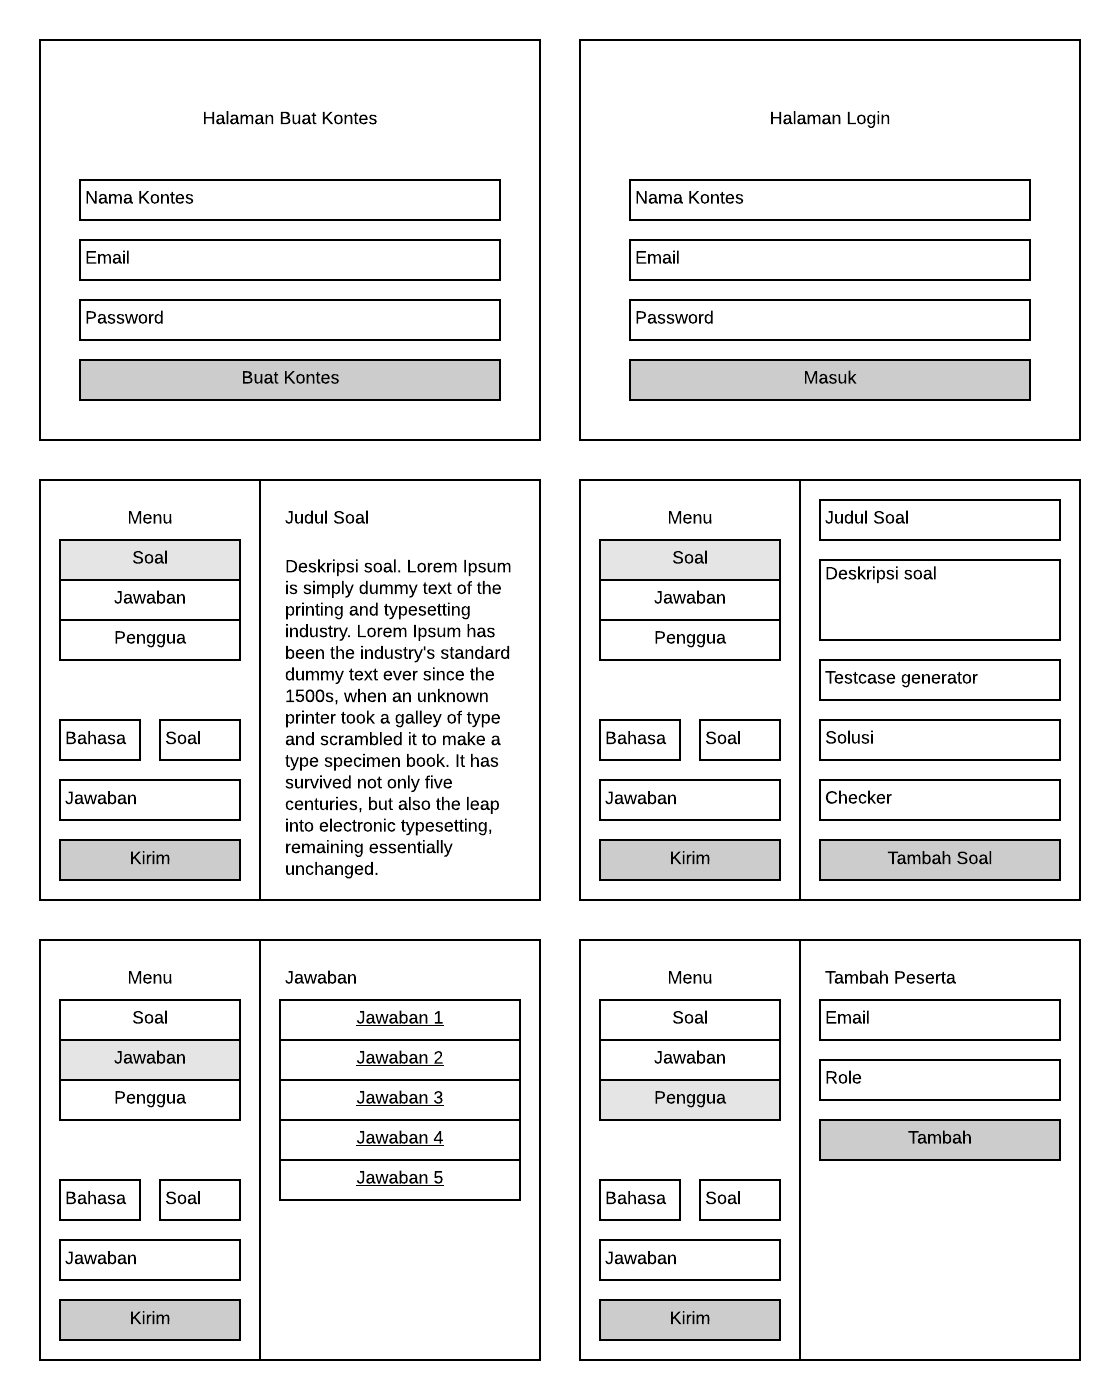
\includegraphics[width=0.85\textwidth]{images/mockup}
    \caption{Desain Tampilan Antar Muka Sistem \textit{Online Judge}.}
    \label{fig:mockup}
\end{figure}

\par Untuk memudahkan peserta dan juri berinteraksi dengan sistem \textit{online judge}, diperlukan komponen antar muka. Pengguna yang merupakan peserta dan juri menggunakan antar muka ini untuk melakukan aksi-aksi pada sistem \textit{online judge}. Kebanyakan sistem \textit{online judge} yang populer saat ini menggunakan antar muka berbasis \textit{web}. Antar muka berbasis \textit{web} digunakan karena mudah diakses oleh pengguna, dan cukup ringan untuk dijalankan.

\par Pada tugas akhir ini, antar muka dibuat dalam bentuk tampilan grafis berbasis web. Untuk memudahkan pengguna, antar muka dibuat sebagai aplikasi \textit{desktop}. Hal ini bertujuan agar komponen antar muka dan \textit{grader} dapat berjalan secara sekaligus. Gambar \ref{fig:mockup} merupakan rancangan halaman-halaman yang dibangun pada komponen antar muka.

% TODO: tambah penjelasan tentang submission, grading_group, grading, erd diagram dari db
    \chapter{Pengembangan Dan Pengujian}

\par Pada tugas akhir ini, perangkat lunak yang dikembangan berupa sistem manajemen kompetisi, \textit{autograder} dan program antarmuka.  Sistem manajemen kompetisi di-\textit{deploy} pada komputer yang disediakan oleh juri dan bertindak sebagai \textit{server}. \textit{Autograder} dan program antarmuka akan didistribusikan kepada peserta dan juri untuk dijalankan pada komputernya. Secara keseluruhan, perangkat lunak yang dikembangkan dinamakan UGrade. Nama tersebut berasal dari kata \textit{you} dan \textit{grade}. Nama tersebut dipilih karena proses penilaian atau \textit{grading} dilakukan oleh masing-masing peserta.

\begin{figure}[ht!]
    \centering
    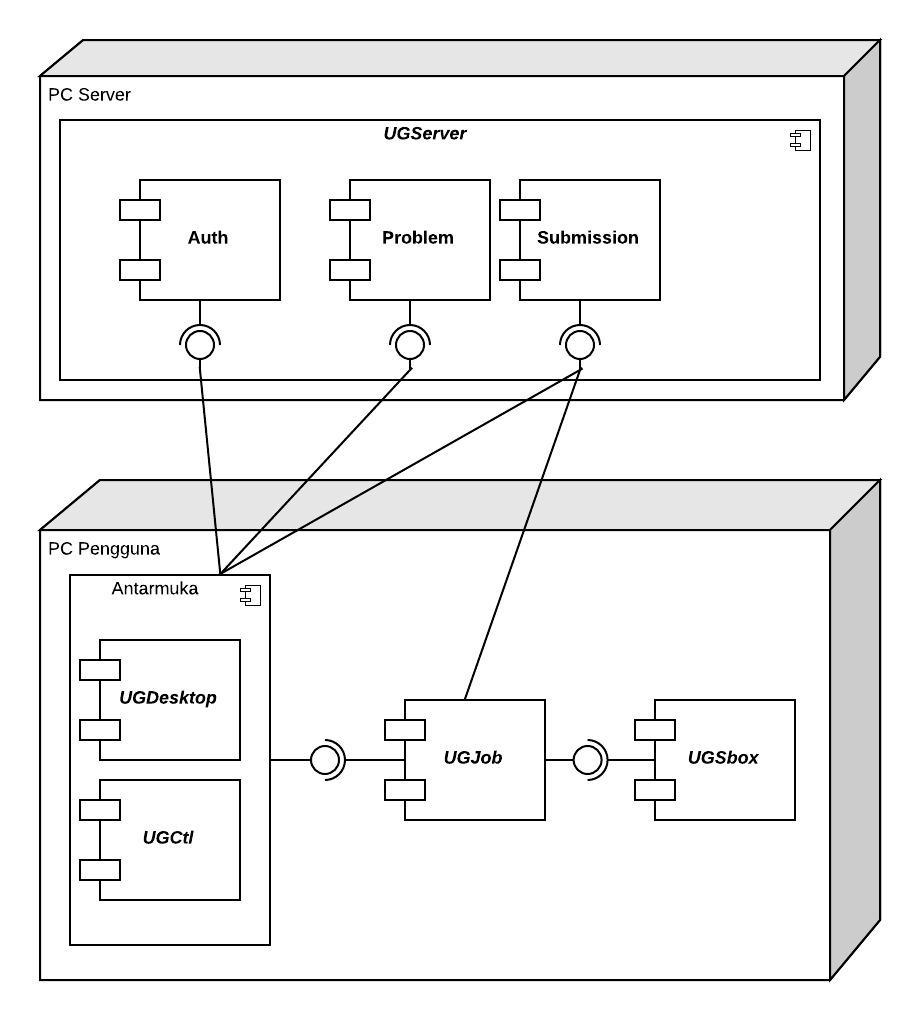
\includegraphics[width=0.8\textwidth]{images/oj-components-impl}
    \caption{Diagram Komponen UGrade}
    \label{fig:oj-components-impl}
\end{figure}

\par Terdapat tiga program utama yang dikembangkan pada UGrade, yaitu: UGServer, UGJob dan UGDesktop. UGServer berfungsi sebagai sistem manajemen kompetisi yang bertindak sebagai \textit{server}. UGJob berfungsi sebagai \textit{worker} dari \textit{autograder}. UGDesktop berfungsi sebagai antarmuka antara pengguna dengan sistem \textit{online judge}. Selain tiga program utama tersebut, terdapat program lain yang digunakan untuk membantu proses pengembangan. Untuk melakukan \textit{sandboxing}, dikembangan program yang bernama UGSbox. Selain itu, untuk memudahkan proses pengujian, dikembangankan program UGCtl yang dapat digunakan pengguna sebagai antarmuka dalam bentuk \textit{command-line}. Gambar \ref{fig:oj-components-impl} merupakan diagram komponen yang menggambarkan keterhubungan program-program yang dibuat pada tugas akhir ini.

\section{UGServer (Sistem Manajemen Kompetisi)}

\par UGServer merupakan sistem manejem kompetisi yang berfungsi untuk mengatur keberjalanan kompetisi. UGServer memberikan layanan kepada peserta dan juri untuk berinteraksi dengan kompetisi. Layanan yang diberikan oleh UGServer antara lain:
\begin{enumerate}
  \item Otentikasi dan otorisasi pengguna.
  \item Pembuatan dan pengaksesan kompetisi.
  \item Pembuatan dan pengaksesan soal pada kompetisi.
  \item Pengiriman dan pengaaksesan jawaban pada kompetisi.
\end{enumerate}

\par Sebenarnya masih banyak layanan lain yang harus diberikan oleh sistem manajemen kompetisi. Akan tetapi, tugas akhir ini lebih difokuskan pada pengembangan \textit{autograder} dibandingkan dengan sistem manajemen kompetisi. Hal ini dikarenakan tujuan dari tugas akhir ini lebih berfokus pada proses penilaian jawaban peserta. Oleh karena itu, fungsionalitas yang dipaparkan pada paragraf di atas sudah cukup untuk memenuhi tujuan dari tugas akhir ini.

\par UGServer dikembangkan dengan menggunakan \textit{framework django}. Pengembangan perangkat lunak berbasis \textit{web} dapat dengan cepat dan mudah dilakukan menggunakan \textit{framework django}. Kemudahan dan kecepatan pengembangan tersebut disebabkan karena \textit{django} telah memberikan banyak fitur yang sangat membantu proses pengembangan perangkat lunak seperti otorisasi, otentikasi, dan ORM (\textit{object relational mapper}). Terdapat beberapa teknologi alternatif lain yang dapat digunakan dan dapat meningkatkan kinerja sistem manajemen kompetisi seperti Express atau Go. Kedua alternatif tersebut tidak digunakan karena membutuhkan waktu pengembangan yang lama dan tidak memberikan peningkatan kinerja yang signifikan. Oleh karena itu, \textit{framework} \textit{django} dipilih untuk mengembangkan UGServer karena mudah dan cepat untuk dikembangkan.

\par UGServer memberikan API (\textit{application programming interface}) yang dapat digunakan oleh pengguna. API yang diberikan oleh UGServer berupa GraphQL yang berjalan di atas protokol HTTP. GraphQL digunakan karena mudah untuk diimplementasikan dan digunakan. UGDesktop dan UGCtl merupakan program antarmuka pengguna yang menggunakan API ini. Terdapat beberapa alternatif lain yang dapat digunakan untuk mengembangkan API dari UGServer seperti menggunakan arsitektur REST (\textit{representational state transfer}) atau menggunakan RPC (\textit{remote procedure call}). Alternatif tersebut tidak digunakan karena tidak fleksibel dan sulit untuk diimplementasikan.

\begin{figure}[ht!]
    \centering
    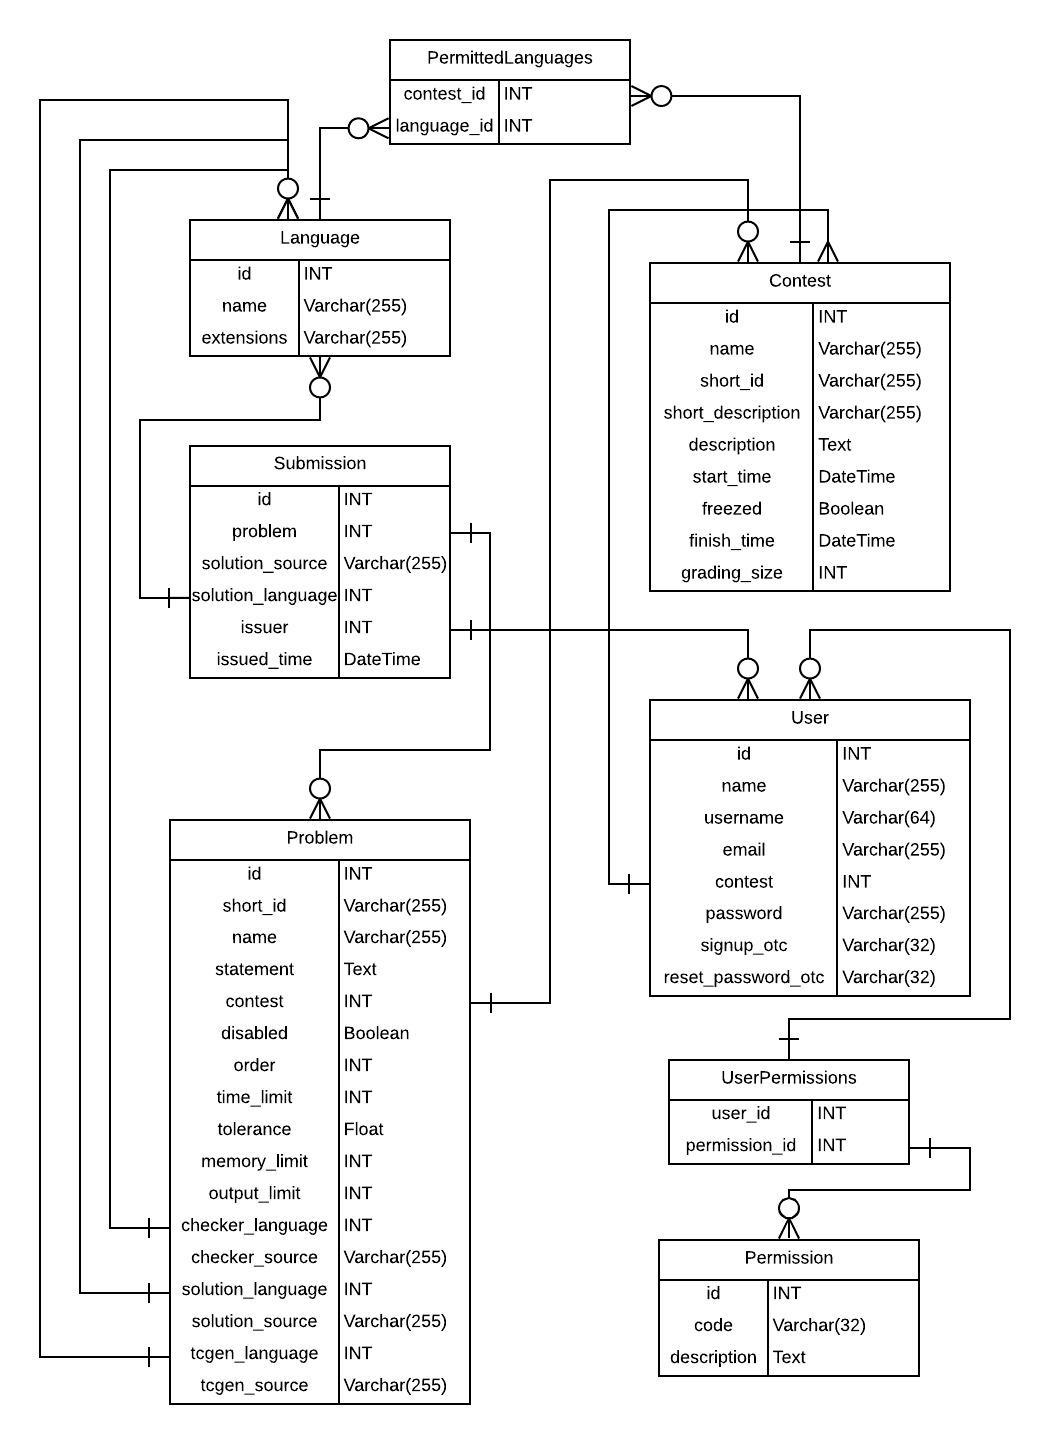
\includegraphics[width=0.8\textwidth]{images/dbschemas}
    \caption{Skema Basis Data Sistem Manajemen Kompetisi}
    \label{fig:dbschemas}
\end{figure}

\par Dalam menjalankan fungsinya, UGServer menggunakan sistem manajemen basis data untuk menyimpan informasi terkait kompetisi. Pada saat ini, UGServer dapat berjalan menggunakan sistem basis data Postgresql atau SQLite. \textit{Framework django} memiliki fitur ORM yang siap digunakan untuk basis data yang bersifat relasional. Karena adanya fitur tersebut, data lebih mudah untuk diatur menggunakan basis data relasional. Oleh karena itu, pada tugas akhir ini penyimpanan data dilakukan dengan memanfaatkan sistem basis data relasional. Gambar \ref{fig:dbschemas} merupakan skema basis data yang digunakan untuk menyimpan informasi terkait kompetisi.

\subsection{Manajemen Pengguna} \label{subsec:user-management}

% akun
\par UGServer memberikan layanan untuk melakukan manajemen pengguna. Pengguna pada UGrade terikat pada suatu kompetisi. Pengguna pada suatu kompetisi tidak dapat mengikuti kompetisi lain. Pengguna yang ingin mengikuti dua buah kompetisi harus membuat dua akun. Pengguna dapat membuat akun dengan cara membuat kompetisi. Ketika seseorang membuat kompetisi, maka sebuah akun akan tercipta sesuai dengan alamat \textit{email} orang tersebut. Selain itu, akun dapat dibuat dengan mengundang orang lain ke dalam kompetisi.

% otentikasi
\par Akun yang pertama kali dibuat hanya mengandung informasi alamat \textit{email} pengguna dan kode untuk otentikasi. Kode tersebut akan dikirim ke \textit{email} pengguna. Hal ini berfungsi sebagai cara untuk mengotentikasi pengguna dengan cara mengotentikasi \textit{email} pengguna. Pengguna kemudian harus memasukkan kode tersebut untuk mengotentikasi dirinya. Pengguna yang telah terotentikasi akan memasukkan informasi mengenai nama lengkap, \textit{username} dan kata sandi. Nama lengkap merupakan nama yang akan ditampilkan pada antarmuka kompetisi. \textit{Username} merupakan nama pengguna yang unik untuk setiap kontes dan bersifat mudah untuk dibaca oleh manusia. Setelah melakukan otentikasi \textit{email}, pengguna selanjutnya dapat melakukan otentikasi dengan kombinasi kompetisi yang diikuti, alamat \textit{email} dan kata sandi yang dipilih. 

% emai + username unik untuk setiap kompetisi
\par Setiap pengguna dalam suatu kompetisi memiliki alamat \textit{email} dan \textit{username} yang unik. Dalam dua kompetisi berbeda bisa saja terdapat akun dengan alamat \textit{email} yang sama. Hal ini dikarenakan akun pengguna terikat pada suatu kompetisi sehingga seorang pengguna dapat diidentifikasi dengan menggunakan informasi kompetisi yang diikutinya dan alamat \textit{email} atau \textit{username}-nya.

\begin{figure}[ht!]
    \centering
    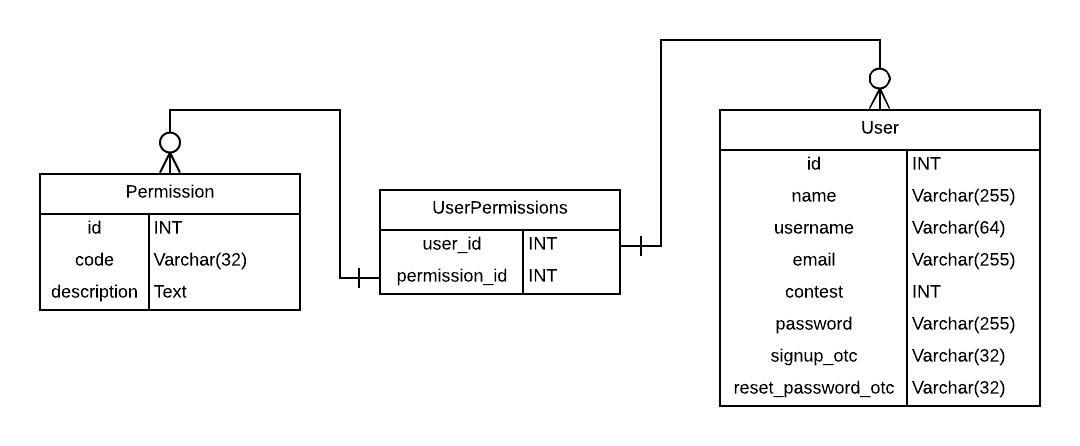
\includegraphics[width=\textwidth]{images/user-schema}
    \caption{Skema Basis Data Sistem Manajemen Pengguna}
    \label{fig:user-schema}
\end{figure}

% user permissions
Pengguna dalam perangkat lunak ini umumnya meliputi juri, peserta dan admin. Perangkat lunak UGServer sebenarnya tidak membeda-bedakan pengguna sebagai juri, peserta ataupun admin. Otorisasi dilakukan dengan memberikan label \textit{permission} kepada setiap pengguna yang ada. Setiap pengguna memiliki himpunan \textit{permission} yang menandakan aksi-aksi apa saja yang dapat dilakukan. Pada saati ini, terdapat beberapa \textit{permission} yang mengatur hak akses pengguna, yaitu:
\begin{enumerate}
    \item \textit{update:contest}: pengguna dengan \textit{permission} ini dapat mengubah informasi kompetisi.
    \item \textit{create:problems}: pengguna dengan \textit{permission} ini dapat membuat soal baru.
    \item \textit{read:problems}: \textit{permission} ini menandakan seorang pengguna dapat melihat dan membaca soal.
    \item \textit{read:disabledProblems}: beberapa soal dapat ditandai sebagai \textit{disabled} sehingga tidak dapat dibaca oleh pengguna yang tidak memiliki \textit{permission} ini.
    \item \textit{update:problems}: pengguna dengan \textit{permission} ini dapat mengubah informasi soal. Soal yang dapat diubah hanyalah soal yang dapat dilihatnya.
    \item \textit{delete:problems}: sebuah soal dapat dihapus oleh pengguna yang memiliki \textit{permission} ini. Soal yang dapat dihapus hanya soal yang dapat dilihat oleh pengguna yang bersangkutan.
    \item \textit{invite:users}: \textit{permission} ini memungkinkan pengguna untuk mengundang pengguna lain.
    \item \textit{update:usersPermissions}: seorang pengguna dapat mengubah \textit{permission} dari pengguna lain jika memiliki \textit{permission} ini.
    \item \textit{delete:users}: pengguna dapat menghapus keanggotaan pengguna lain jika memiliki \textit{permission} ini.
    \item \textit{read:submissions}: dengan \textit{permission} ini, pengguna dapat melihat semua jawaban pengguna lain. \textit{Permission} ini biasanya diberikan untuk juri.
    \item \textit{create:submissions}: \textit{permission} ini memungkinkan pengguna untuk mengirimkan jawabannya. Pengguna tanpa \textit{permission} ini dapat dipandang sebagai seorang penonton.
\end{enumerate}
Pemberian \textit{permission} untuk setiap pengguna bertujuan untuk meningkatkan \textit{granularitas} pada hak akses untuk setiap pengguna. Gambar \ref{fig:user-schema} merupakan skema basis data yang digunakan untuk melakukan manajemen pengguna.

% TODO: jelasin API

\subsection{Manajemen Soal}

\begin{figure}[ht!]
    \centering
    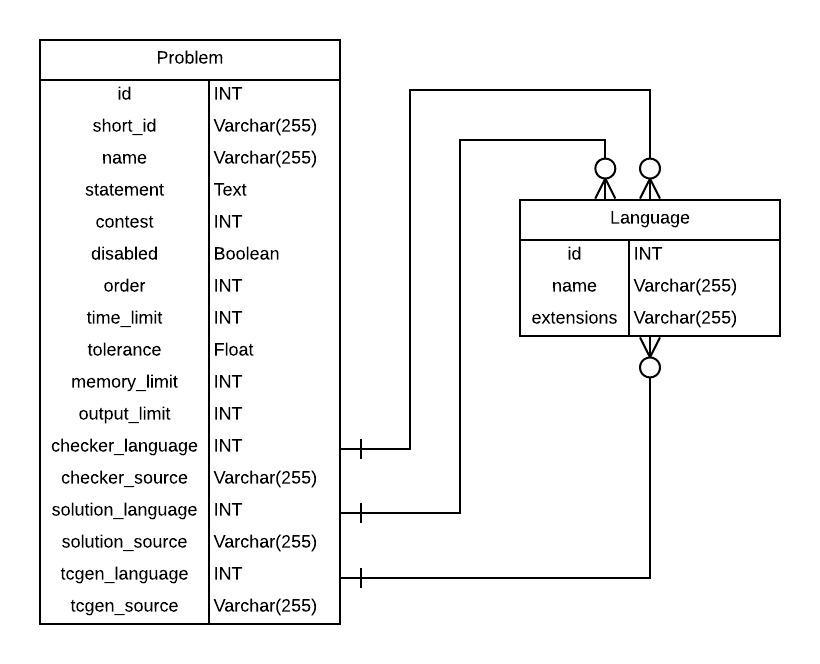
\includegraphics[width=0.8\textwidth]{images/problem-schema}
    \caption{Skema Basis Data Sistem Manajemen Soal}
    \label{fig:problem-schema}
\end{figure}

\par Setiap soal pada UGServer akan terikat pada suatu kompetisi. Suatu soal tidak dapat berada pada dua kompetisi sekaligus. Jika terdapat soal yang sama pada kompetisi yang berbeda, maka soal tersebut harus ditambahkan dua kali dan tetap dianggap soal yang berbeda. Setiap soal pada kompetisi memiliki nama dan \textit{short id}. Nama soal merupakan judul soal yang akan ditampilkan pada sistem antarmuka yang digunakan pengguna. \textit{Short id} merupakan kode soal yang unik untuk setiap kompetisi dan mudah untuk dibaca oleh manusia. \textit{Short id} berguna untuk mengidentifikasi soal dengan mudah.

\par Informasi mengenai soal disimpan di sistem basis data pada tabel \textit{problems}. Skema basis data yang digunakan untuk menyimpan informasi soal digambarkan pada Gambar \ref{fig:problem-schema}. Aksi-aksi yang dapat dilakukan oleh pengguna terhadap soal ditentukan berdasarkan \textit{permission} yang dimiliki oleh pengguna tersebut.

\begin{figure}[ht!]
    \centering
    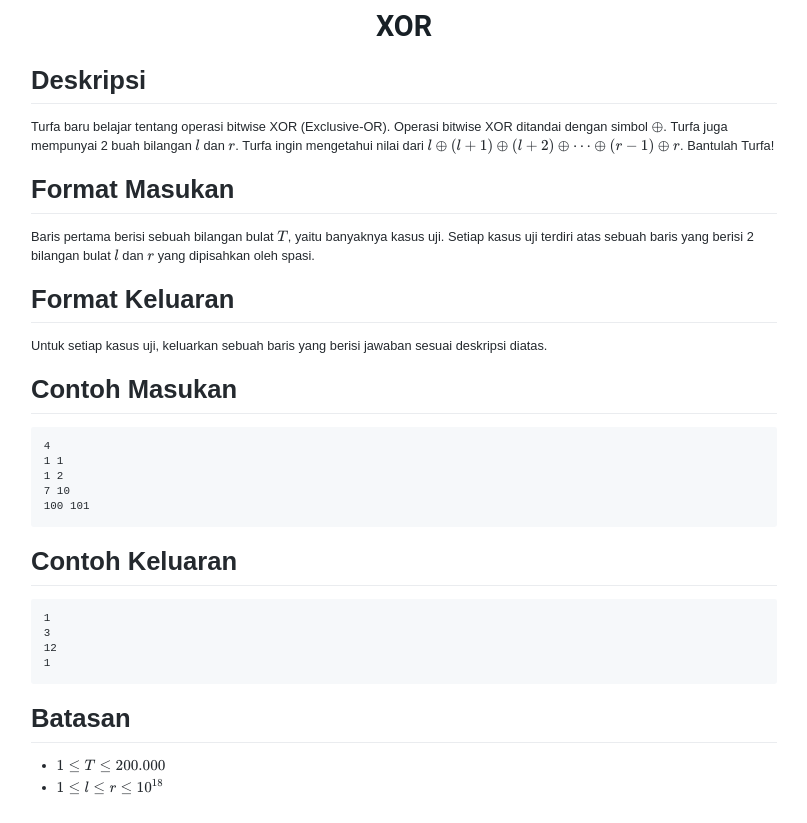
\includegraphics[width=\textwidth]{images/problem-desc-example}
    \caption{Contoh Deskripsi Soal.}
    \label{fig:problem-desc-example}
\end{figure}

\par Setiap soal memiliki deskripsi soal. Deskripsi soal merupakan penjelasan mengenai soal, format masukan, format keluaran, contoh masukan dan contoh keluaran. Deskripsi soal ditulis dalam format \textit{markdown} dan disimpan pada \textit{field} \textit{statement} pada tabel \textit{problems}. Pemilihan format \textit{markdown} bertujuan untuk kemudahan melakukan penyimpanan deskripsi soal. Beberapa sistem \textit{online judge} lain memungkinkan melakukan penyimpanan soal dalam bentuk \textit{file} seperti \textit{pdf}. UGServer tidak mendukung penyisipan \textit{file} pada deskripsi soal. Hal ini bertujuan untuk memudahkan implementasi. Gambar \ref{fig:problem-desc-example} merupakan contoh deskripsi soal.

\par Untuk melakukan penilaian terhadap jawaban peserta, setiap soal dilengkapi dengan beberapa informasi terkait penilaian. Beberapa informasi yang terkait dengan penilaian adalah: batas waktu eksekusi, batas penggunaan memori, batas \textit{output file} yang dihasilkan, faktor toleransi, \textit{testcase generator}, solusi juri dan \textit{checker}. Batas waktu eksekusi disimpan pada \textit{field timelimit} dalam bentuk bilangan bulat yang menyatakan lamanya batas waktu eksekusi dalam satuan milidetik. Batas waktu ini digunakan oleh \textit{autograder} untuk menghentikan program secara paksa ketika berjalan terlalu lama. Batas penggunaan memori dan \textit{output file} yang dihasilkan disimpan pada \textit{field memorylimit} dan \textit{outputlimit} di tabel \textit{problems}. Batas tersebut disimpan dalam bentuk bilangan bulat yang menyatakan batas dalam satuan \textit{bytes}. Faktor toleransi disimpan pada \textit{field tolerance} di tabel \textit{problems} sebagai \textit{float}.

\par Dalam melakukan penilaian, \textit{autograder} memerlukan informasi mengenai \textit{testcase generator}, solusi juri, dan \textit{checker}. Informasi tersebut berupa \textit{source code} pada bahasa pemrograman tertentu. UGServer menyimpan informasi bahasa pemrograman yang digunakan oleh \textit{testcase generator}, solusi juri dan \textit{checker} pada sistem basis data sebagai \textit{foreign key} ke tabel \textit{languages}. Informasi bahasa pemrograman tersebut disimpan pada \textit{field tcgen\_language, solution\_language}, dan \textit{checker\_language} di tabel \textit{problems}. Informasi mengenai kode sumber tidak disimpan dalam sistem basis data karena dianggap kurang efisien jika ukuran \textit{source code} terlalu besar. Oleh karena itu, kode sumber disimpan sebagai \textit{file} yang disimpan di \textit{disk}. Dengan begitu, sistem basis data hanya perlu menyimpan informasi mengenai alamat \textit{file} dari \textit{source code} yang disimpan.

% TODO: graphql API

\par Pengguna dapat melakukan beberapa aksi pada soal yang ada pada sistem seperti: melihat daftar soal, membaca soal, menambah soal, mengubah soal, dan menghapus soal. Pengguna hanya dapat melakukan aksi-aksi tersebut sesuai izin yang dimilikinya seperti yang sudah dijelaskan pada bagian \ref{subsec:user-management}. Aksi-aksi tersebut dapat dilakukan dengan memanfaatkan API GraphQL yang ada pada UGServer.

\subsection{Manajemen Jawaban}

\par Peserta maupun juri dapat mengirimkan jawabannya terhadap suatu soal jika memiliki \textit{permission create:submissions}. Jawaban terhadap suatu soal berupa \textit{source code} yang ditulis pengguna dalam bahasa pemrograman tertentu yang diizinkan. Pada saat ini, bahasa pemrograman yang dapat digunakan adalah C dan C++. Pengguna dapat mengirimkan jawaban melalui API GraphQL yang ada pada UGServer.

\begin{figure}[ht!]
    \centering
    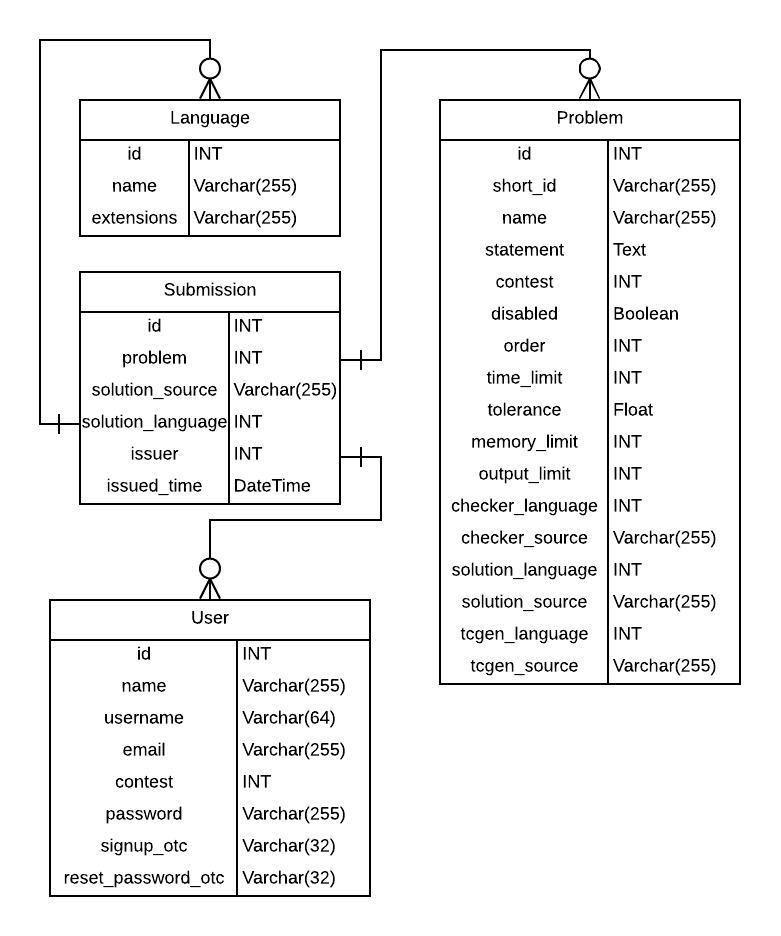
\includegraphics[width=0.8\textwidth]{images/submission-schema}
    \caption{Skema Basis Data Sistem Manajemen Jawaban}
    \label{fig:submission-schema}
\end{figure}

\par \textit{Source code} dari jawaban dari pengguna akan disimpan dalam bentuk \textit{file} yang berada pada \textit{disk}. Selain \textit{source code}, terdapat informasi lain pada jawaban pengguna yang disimpan seperti bahasa pemrograman yang digunakan, waktu pengiriman jawaban, pengirim jawaban dan soal yang bersangkutan. Informasi tersebut disimpan dalam basis data pada tabel \textit{submission}. Gambar \ref{fig:submission-schema} merupakan skema basis data yang digunakan untuk menyimpan jawaban.

\par Setiap jawaban yang berhasil dikirim oleh pengguna akan dinilai oleh \textit{grader}. \textit{Grader} akan berjalan secara otomatis ketika jawaban peserta disimpan. \textit{Grader} kemudian akan menentukan \textit{verdict} dari jawaban peserta. \textit{Verdict} merupakan hasil penilaian terhadap jawaban peserta. Jenis \textit{verdict} yang digunakan adalah:
\begin{enumerate}
    \item \textit{Accpeted}: menandakan bahwa jawaban memberikan keluaran yang benar, memenuhi batasan dan dianggap sebagai jawaban yang benar.
    \item \textit{Wrong Answer}: menandakan bahwa jawaban memberikan keluaran yang salah tetapi memenuhi batasan.
    \item \textit{Memory Limit Exceeded}: menandakan bahwa jawaban menggunakan terlalu banyak memori dan melebihi batasan yang ditetapkan oleh juri.
    \item \textit{Time Limit Exceeded}: menandakan bahwa jawaban melebihi batasan waktu yang sudah ditetapkan.
    \item \textit{Runtime Error}: menandakan bahwa jawaban tidak berhasil dieksekusi karena jawaban memiliki kesalahan dan menimbulkan \textit{error} pada saat jawaban dieksekusi.
    \item \textit{Compile Error}: menandakan jawaban tidak dapat dikompilasi.
    \item \textit{Internal Error}: menandakan adanya kesalahan pada sistem UGrade sehingga jawaban tidak dapat dinilai.
\end{enumerate}

\subsection{Penilaian Jawaban}

\par Setiap jawaban yang dikirimkan oleh pengguna akan dinilai secara otomatis oleh UGServer. Penilaian dilakukan secara \textit{asynchronous}. Oleh karena itu, peserta tidak perlu menunggu penilaian selesai untuk melakukan aksi-aksi lain. Seringkali terdapat beberapa masalah teknis yang mengakibatkan jawaban peserta perlu dinilai ulang. Oleh sebab itu, setiap jawaban peserta dapat dinilai lebih dari satu kali. Hasil penilaian yang digunakan adalah hasil penilaian yang terakhir.

\subsubsection{\textit{Grading Group}}

\par Penilaian pada sebuah jawaban disebut sebagai \textit{grading group}. Setiap jawaban dapat dinilai lebih dari satu kali dan memiliki lebih dari satu \textit{grading group}. Adanya \textit{grading group} berguna untuk melakukan penilaian terhadap jawaban peserta lebih dari satu kali. Jika terdapat perubahan \textit{testcase} atau perubahan batasan waktu pada suatu soal, maka perlu adanya penilaian ulang. Penilaian ulang dapat dilakukan dengan membuat \textit{grading group} baru untuk setiap penilaian.

\begin{figure}[ht!]
    \centering
    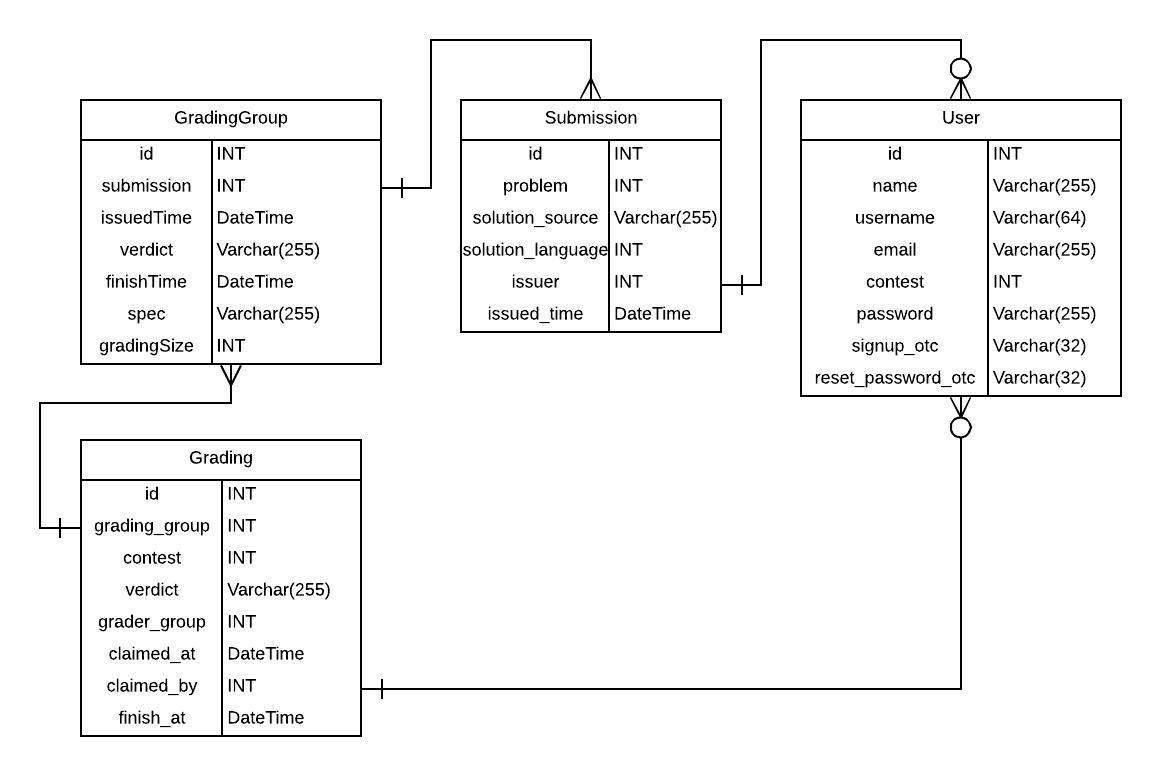
\includegraphics[width=\textwidth]{images/grader-schema}
    \caption{Skema Penilaian Jawaban Pengguna}
    \label{fig:grader-schema}
\end{figure}

\par Informasi dari \textit{grading group} disimpan dalam tabel \textit{GradingGroups} pada sistem basis data. Setiap \textit{grading group} memiliki informasi mengenai jawaban peserta, catatan waktu terciptanya \textit{grading group}, \textit{verdict}, spesifikasi penilaian, catatan waktu selesainya penilaian, dan \textit{grading size}. Informasi-informasi tersebut disimpan sebagai \textit{field} dalam tabel \textit{GradingGroups}. Spesifikasi penilaian berupa \textit{archive file} dan disimpan sebagai \textit{file} dalam \textit{disk}. Field \textit{spec} pada tabel \textit{GradingGroups} menyimpan informasi alamat \textit{file} dari spesifikasi penilaian. Skema basis data yang digunakan untuk melakukan penilaian ditunjukkan pada Gambar \ref{fig:grader-schema}.

\par Penilaian diawali dengan pembuatan spesifikasi penilaian. Spesifikasi penilaian berisi informasi mengenai \textit{testcase generator}, solusi juri, \textit{checker}, solusi peserta dan batasan soal. Informasi tersebut disimpan sebagai \textit{file} dengan format \textit{tar}. Spesifikasi penilaian tersebut terdiri dari beberapa file sebagai berikut:
\begin{enumerate}
    \item tcgen.cpp\\ merupakan kode sumber \textit{testcase generator} dari soal. Ekstensi dari \textit{file} dapat berbeda sesuai bahasa pemrograman yang digunakan.
    \item solution.cpp\\ merupakan kode sumber  solusi juri pada soal yang bersangkutan. Ekstensi dari \textit{file} dapat berbeda sesuai bahasa pemrograman yang digunakan.
    \item checker.cpp\\ merupakan kode sumber \textit{checker} dari soal. Ekstensi dari \textit{file} dapat berbeda sesuai dengan bahasa pemrograman yang digunakan.
    \item submission.cpp\\ merupakan kode sumber solusi peserta. Ekstensi dari \textit{file} dapat berbeda sesuai dengan bahasa pemrograman yang digunakan.
    \item lang.json\\ berupa \textit{file} yang berisi dokumen JSON (\textit{javascript object notation} dan berisi informasi bahasa pemrograman yang digunakan sebagai \textit{testcase generator}, solusi juri, \textit{checker} dan solusi peserta. Dokumen JSON pada \textit{file} ini hanya berisi empat \textit{key}, yaitu \textit{tcgen}, \textit{solution}, \textit{checker}, dan \textit{submission}. Setiap \textit{key} pada \textit{file} ini memiliki \textit{value} yaitu ID dari bahasa pemrograman yang digunakan.
    \item problem.json\\ berupa \textit{file} yang berisi dokumen JSON dan berisi informasi batasan dari soal. Dokumen JSON pada file ini berisi empat buah \textit{key}, yaitu \textit{timeLimit}, \textit{outputLimit}, \textit{memoryLimit}, dan \textit{tolerance}. Setiap \textit{key} pada \textit{file} ini memiliki \textit{value}  berupa bilangan yang menjelaskan batasan dari soal.
\end{enumerate}
\par \textit{File} spesifikasi penilaian ini nantinya diunduh oleh \textit{autograder} yang berjalan pada komputer pengguna.

\subsubsection{\textit{Grading Size}}

\par Setiap penilaian yang ditandai dengan \textit{grading group} memiliki suatu nilai \textit{grading size}. Nilai dari \textit{grading size} digunakan untuk mengurangi risiko serangan yang mungkin dilakukan pengguna. Sebuah penilaian dapat dilakukan oleh lebih dari satu \textit{worker}. Setiap worker akan memberikan hasil penilaiannya kepada UGServer. Jawaban peserta akan dinilai benar ketika mayoritas dari \textit{worker} yang melakukan penilaian memberikan \textit{verdict} \textit{accepted}. Nilai dari \textit{grading size} mengindikasikan banyaknya \textit{worker} yang melakukan penilaian.

\par Nilai \textit{grading size} yang besar akan lebih aman karena dapat lebih mengurangi risiko kecurangan peserta. Hal ini dikarenakan kemungkinan terjadinya kecurangan lebih kecil sebab \textit{worker} yang bekerja lebih banyak. Meskipun begitu, tingginya nilai \textit{grading size} menyebabkan proses penilaian menjadi lebih lambat karena penilaian harus menunggu banyak \textit{worker} untuk selesai terlebih dahulu. Sebaliknya, nilai \textit{grading size} yang kecil dapat mempercepat penilaian akan tetapi mengurangi keamanan. Nilai \textit{grading size} dapat diatur dalam pengaturan kompetisi oleh pengguna yang memiliki \textit{permission} \textit{update:contests}.

\par Karena setiap jawaban dapat dinilai lebih dari satu kali, perlu ada entitas yang merepresentasikan penilaian sebuah jawaban oleh sebuah \textit{worker}. Entitas tersebut dinamakan \textit{grading}. Sebuah \textit{grading} memiliki informasi mengenai \textit{grading group} terkait, \textit{verdict}, \textit{grader group}, catatan waktu penilaian, dan pengguna yang melakukan penilaian. Informasi ini disimpan di dalam basis data pada tabel \textit{Gradings}.

\par Secara singkat, setiap jawaban dapat memiliki beberapa \textit{grading group} yang merepresentasikan sebuah penilaian terhadap jawaban. Hasil penilaian jawaban pada sebuah \textit{grading group} merupakan hasil penilaian yang dilakukan oleh banyak \textit{worker}. Banyaknya \textit{worker} yang melakukan penilaian adalah sebanyak \textit{grading size}. Setiap penilaian yang dilakukan oleh \textit{worker} direpresentasikan menjadi sebuah \textit{grading}. Secara singkat dapat dikatakan bahwa setiap \textit{grading group} memiliki \textit{grading} sebanyak \textit{grading size}.

\subsubsection{\textit{Grader Group}}

\par Adanya nilai dari \textit{grading size} bertujuan agar setiap jawaban dapat dinilai lebih dari satu \textit{worker}. \textit{Worker} yang melakukan penilaian terhadap suatu jawaban tentunya harus merupakan \textit{worker} yang berbeda. Untuk mengatasi hal ini, setiap \textit{grading} dan \textit{worker} memiliki sebuah nilai \textit{grader group}. \textit{Worker} dengan nilai \textit{grader group} tertentu hanya dapat melakukan penilaian terhadap \textit{grading} yang memiliki nilai \textit{grader group} yang sama. Setiap penilaian jawaban peserta, akan dibuat \textit{grading size} buah \textit{grading} yang memiliki nilai \textit{grader group} yang unik yaitu dari nol hingga $\textit{grading size} - 1$. Setiap \textit{worker} dengan \textit{grader group} $K$ hanya akan melakukan penilaian terhadap \textit{grading} yang memiliki nilai \textit{grader group} $K$.

\par Nilai \textit{grader group} dari setiap \textit{worker} dihitung dengan cara melakukan \textit{hash} pada ID \textit{worker}. Setiap \textit{worker} memiliki ID berupa bilangan bulat yang unik. Nilai \textit{grader group} sebuah worker dihitung dengan formula $\textit{grader\_group} = hash(W_{id}) \bmod \textit{grading\_size}$. Dengan mengasumsikan jumlah \textit{worker} cukup banyak dibandingkan dengan nilai \textit{grading size}, cara ini akan mengelompokkan seluruh \textit{worker} menjadi \textit{grading size} buah kelompok dengan anggota yang kira-kira sama banyak. Cara ini dipilih karena perhitungannya yang cepat, mudah dan dapat mengelompokkan \textit{worker} secara rata.

\begin{figure}[ht!]
    \centering
    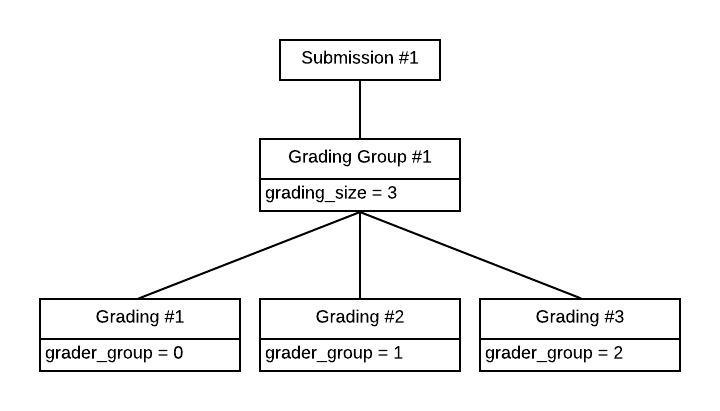
\includegraphics[width=0.6\textwidth]{images/grading-example-1}
    \caption{Contoh Proses Pembuatan \textit{Grading}}
    \label{fig:grading-example-1}
\end{figure}

\par Sebagai contoh, seorang pengguna telah melakukan pengiriman jawaban terhadap suatu soal. Setelah pengiriman jawaban tersebut berhasil dilakukan, akan tercipta sebuah \textit{submission} yang dapat kita beri nama \textit{Submission \#1}. UGServer kemudian akan secara otomatis membuat \textit{grading group} untuk menilai jawaban tersebut. Kita dapat memisalkan \textit{grading group} tersebut bernama \textit{Grading Group \#1}. Pada \textit{Grading Group \#1} terdapat informasi mengenai \textit{grading size}. Informasi \textit{grading size} didapatkan dari konfigurasi kompetisi. Pengguna dengan \textit{permission update:contest} dapat mengubah nilai ini. Dalam contoh ini, nilai \textit{grading size} dari kompetisi tersebut adalah tiga. Setelah \textit{grading group} terbentuk, UGServer akan membuat \textit{grading size} buah \textit{grading}. Dalam contoh ini berarti akan tercipta tiga buah \textit{grading}. Untuk kemudahan penjelasan, tiga buah \textit{grading} ini dapat kita sebut dengan \textit{Grading \#1} , \textit{Grading \#2}, dan \textit{Grading \#3}. Setiap \textit{grading} yang diciptakan akan memiliki nilai \textit{grader group} yang unik dan terurut dari nol hingga $\textit{grading size} - 1$. Dalam contoh ini \textit{Grading \#1} memiliki nilai \textit{grader group} nol, \textit{Grading \#2} memiliki nilai \textit{grader group} satu, dan \textit{Grading \#3} memiliki nilai \textit{grader group} dua. Gambar \ref{fig:grading-example-1} menggambarkan \textit{submission}, \textit{grading group} dan \textit{grading} pada contoh di paragraf ini.

\begin{figure}[ht!]
    \centering
    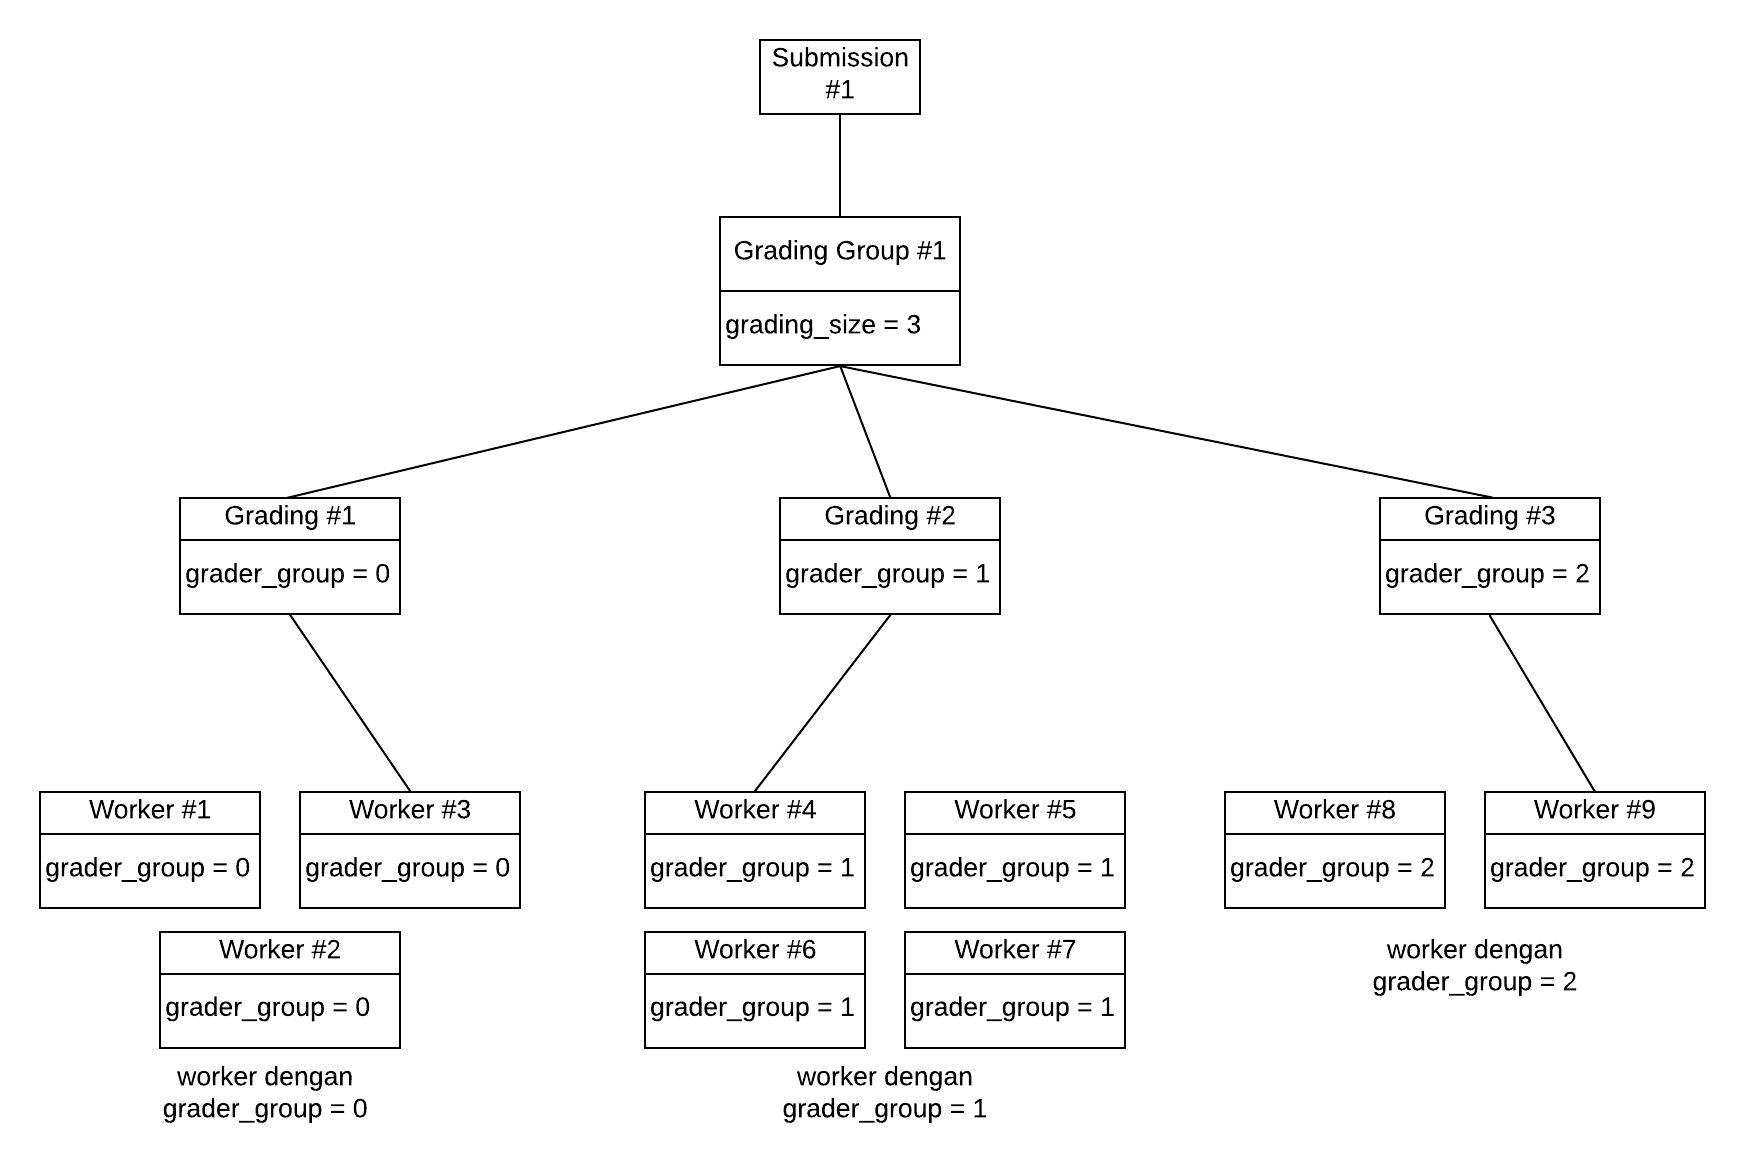
\includegraphics[width=\textwidth]{images/grading-example-2}
    \caption{Contoh Proses Penilaian Oleh \textit{Worker}}
    \label{fig:grading-example-2}
\end{figure}

\par Setelah terbentuk tiga buah \textit{grading} seperti pada paragraf sebelumnya, penilaian dapat mulai dilakukan oleh \textit{worker}. \textit{Worker} secara periodik akan selalu bertanya pada UGServer apakah terdapat \textit{grading} yang perlu dikerjakan. UGServer akan memberikan \textit{grading} yang sesuai dengan nilai dari \textit{grader group} \textit{worker} yang bersangkutan. Setiap \textit{grading} memiliki informasi \textit{claimed\_by} yang akan berisi ID dari peserta yang sedang melakukan penilaian terhadap \textit{grading} tersebut. Nilai tersebut bertujuan agar \textit{grading} yang sedang dinilai tidak akan dinilai oleh \textit{worker} lain. Gambar \ref{fig:grading-example-2} menjelaskan pemberian \textit{grading} pada \textit{worker} yang dilakukan oleh UGServer.

\par \textit{Worker} yang telah melakukan penilaian akan mengirimkan hasil penilaiannya kepada UGServer. UGServer kemudian akan mengubah nilai \textit{verdict} dari \textit{grading} dan mencatat waktu selesainya penilaian. Jika jumlah \textit{grading} yang selesai dinilai sudah lebih dari setengah dari \textit{grading size}, maka \textit{verdict} dari \textit{grading group} akan diubah. Setelah tahap tersebut, pengguna dapat melihat hasil akhir penilaiannya. 

% TODO: jelasin API waktu grading

% TODO: use more clear term for worker, grading group, grading size, grading, grader group.

% TODO: tambah kode assign grader group

% TODO: further works

\section{UGSbox}

% TODO: jelasin kodenya

\par Dalam menjalankan penilaian, UGSbox berperan dalam memberikan isolasi terhadap program-program yang berjalan di komputer pengguna. Program-program yang berjalan pada saat penilaian antara lain adalah: \textit{compiler}, \textit{testcase generator}, solusi peserta, solusi juri, dan \textit{checker}. Program-program ini dapat berisi kode yang membahayakan komputer pengguna yang menjalankannya. Oleh karena itu, diperlukan adanya sistem yang dapat mengisolasi program tersebut sehingga tidak membahayakan komputer pengguna. Pada tugas akhir ini, UGSbox berperan dalam memberikan isolasi tersebut.

\par UGSbox memberikan isolasi pada proses yang berjalan dengan menggunakan beberapa fitur dari Linux. Isolasi yang diberikan UGSbox antara lain adalah sebagai berikut:
\begin{itemize}
    \item isolasi \textit{filesystem}. \\ Isolasi terhadap \textit{filesystem} dilakukan dengan menggunakan \textit{system call chroot}. Dengan menggunakan \textit{chroot}, direktori \textit{root} dari suatu  proses dapat diganti menjadi direktori lain. Mengganti \textit{root} dari proses mengakibatkan proses tersebut tidak dapat mengakses \textit{file} yang ada di luar \textit{root}. \textit{Filesystem} yang akan digunakan oleh proses dapat dimuat dari \textit{file} yang memiliki format \textit{tar.xz}. \textit{File} tersebut dinamakan \textit{image file}. Proses isolasi \textit{filesystem} dimulai dengan melakukan ekstraksi \textit{image file} kemudian mengganti \textit{root} dari proses ke dalam direktori \textit{image file} yang sudah berhasil diekstrak. 

    \item \textit{Filesystem binding}. \\ UGSbox memberikan fitur \textit{filesystem binding} yang dapat digunakan oleh pengguna untuk memasukkan \textit{filesystem} lain ke dalam \textit{filesystem} yang sudah diisolasi. Fitur ini berguna untuk menyimpan \textit{testcase} ke dalam suatu \textit{filesystem} khusus yang kemudian dapat dimuat ke dalam \textit{filesystem} yang sudah diisolasi.

    \item Isolasi \textit{network}. \\ Untuk menjaga keamanan, setiap proses yang berjalan di dalam lingkungan yang diisolasi tidak boleh menggunakan \textit{network} untuk berkomunikasi dengan dunia luar. Untuk mengatasi masalah ini, UGSbox menggunakan fitur \textit{namespace} dari Linux. Proses yang diisolasi akan mendapat \textit{namespace} dengan \textit{network interface} yang terisolasi dari \textit{network interface} milik \textit{host}.

    \item Isolasi \textit{user}. \\ Selain isolasi \textit{network}, \textit{namespace} pada Linux juga digunakan untuk melakukan isolasi \textit{user}. Dengan mengisolasi \textit{user}, proses yang terisolasi tidak dapat mengetahui adanya \textit{user} lain di luar lingkungannya.

    \item Batas penggunaan CPU dan memori. \\ Penggunaan CPU dan memori dari proses yang diisolasi tentunya perlu dibatasi. Hal ini bertujuan agar proses yang berjalan tidak memberatkan komputer pengguna ketika penilaian sedang berlangsung. Untuk mengatasi masalah ini, UGSbox menggunakan fitur \textit{cgroup} dari Linux. Dengan menggunakan \textit{cgroup}, penggunaan memori dan CPU dari suatu proses dapat dibatasi dan diawasi. Proses yang menggunakan CPU atau memori melebihi batasan akan dihentikan secara paksa. 

    \item Batas ukuran \textit{file} yang dapat dihasilkan. \\ Program yang dikirimkan oleh pengguna mungkin saja memuat kode yang dapat memberatkan \textit{disk} karena melakukan penulisan secara terus menerus. Hal ini dapat mengakibatkan komputer pengguna menjadi lambat karena \textit{disk}-nya tidak dapat digunakan. Untuk mengatasi masalah ini, UGSbox membatasi ukuran \textit{file} yang dapat diciptakan oleh proses di dalam lingkungan yang diisolasi. Pembatasan ini dicapai dengan menggunakan \textit{system call setrlimit}.

    \item Batas jumlah \textit{file} yang dapat dibuka. \\ Untuk meningkatkan keamanan, jumlah \textit{file} yang dapat dibuka oleh proses yang diisolasi juga dibatasi menggunakan \textit{system call setrlimit}.

    \item Batas proses yang dapat diciptakan. \\ Selain membatasi ukuran \textit{file} yang dihasilkan, dan jumlah \textit{file} yang dapat dibuka, UGSbox juga menggunakan \textit{setrlimit} untuk membatasi jumlah proses yang dapat diciptakan.

\end{itemize}

\begin{lstlisting}[caption={Contoh Hasil Eksekusi Perintah \textit{ugsbox guard}},label={lst:ugsbox-guard},language=Bash,style=BashStyle]
$ ugsbox guard --help
Usage:
  ugsbox guard [flags]

Flags:
  -b, --bind strings               bind host directory to sandbox directory with format <hostdir>:<sandboxdir>. Warning: file owner of binded directory will be changed
  -f, --file-size uint             generated file size limit
  -h, --help                       help for guard
  -i, --image string               compressed sandbox image (in .tar.xz) path
  -m, --memory-limit uint          memory limit in bytes (default 67108864)
  -M, --memory-throttle uint       memory throttle in bytes (default 268435456)
  -n, --nproc uint                 limit process creation e.g.: fork/exec
  -o, --open-file uint             open file limit
  -s, --stack-size uint            limit stack size in bytes
  -E, --stderr string              path (relative to sandbox) to file to be used as stderr
  -I, --stdin string               path (relative to sandbox) to file to be used as stdin
  -O, --stdout string              path (relative to sandbox) to file to be used as stdout
  -t, --time-limit uint            time limit in milisecond (default 10000)
  -T, --walltime-limit uint        wall clock time limit in milisecond (default 10000)
  -w, --working-directory string   working directory of process (default "/home")

Global Flags:
      --debug   show debug log
      --trace   show trace log
\end{lstlisting}

\par UGSBox dapat digunakan dengan dua cara, yaitu sebagai \textit{executable program} atau sebagai \textit{library}. Pengguna dapat menggunakan perintah \textit{ugsbox guard} untuk menjalankan UGSbox melalui CLI (\textit{command line interface}). Kode \ref{lst:ugsbox-guard} merupakan contoh hasil pemanggilan \textit{ugsbox guard}.

\par Selain melalui CLI, UGSbox juga dapat digunakan melalui pemanggilan fungsi pada bahasa pemrograman Go. Untuk dapat menggunakan UGSbox sebagai \textit{library}, pengguna dapat meng-\textit{import} \textit{package github.com/jauhararifin/ugrade/sandbox}. Dokumentasi penggunaan \textit{library} tersebut dapat dapat diakses menggunakan \textit{web browser} pada alamat berikut: \textit{https://godoc.org/github.com/jauhararifin/ugrade}.

\section{UGJob}

% TODO: jelasin kodenya

\par UGJob merupakan hasil implementasi dari \textit{autograder} pada keluarga perangkat lunak UGrade. UGJob dikembangkan menggunakan bahasa Go dan berperan dalam menilai jawaban pengguna. UGJob dikembangkan sebagai sebuah \textit{executable} yang dapat dijalankan melalui CLI. UGDesktop akan secara periodik menjalankan UGJob untuk melakukan penilaian.

\par Setiap \textit{grading} yang dihasilkan oleh UGServer akan dinilai oleh \textit{worker} yang ada pada komputer pengguna. \textit{Worker} pada komputer pengguna tidak perlu mengetahui adanya konsep \textit{grading group}, \textit{grading size}, dan \textit{grader group}. \textit{Worker} hanya perlu meminta \textit{grading} pada UGServer untuk dinilai. Dalam meminta \textit{grading}, \textit{worker} hanya perlu mengirimkan ID dari pengguna yang bertindak sebagai \textit{worker}. UGServer akan memberikan \textit{grading} yang sesuai dengan ID pengguna dari \textit{worker} tersebut.

\par Di sisi \textit{worker}, semua \textit{grading} yang perlu dinilai akan dipandang sebagai sebuah \textit{job}. Pada tugas akhir ini, \textit{job} dapat disamakan dengan \textit{grading} karena sebuah \textit{grading} akan dianggap sebagai sebuah \textit{job} oleh \textit{worker}. Istilah \textit{job} digunakan untuk meningkatkan abstraksi dari \textit{worker}. \textit{Worker} tidak perlu mengetahui konsep penilaian yang dilakukan di sisi UGServer. \textit{Worker} tidak perlu mengetahui adanya konsep \textit{grading} yang ada pada UGServer. Semua penilaian yang perlu dilakukan oleh \textit{worker} akan dianggap sebagai sebuah \textit{job}. Dengan menggunakan istilah \textit{job}, sistem penilaian yang ada pada sisi UGServer dapat dengan mudah dimodifikasi tanpa memengaruhi \textit{worker}.

\begin{lstlisting}[caption={Contoh Hasil Eksekusi Perintah \textit{ugjob consume}},label={lst:ugjob-consume},language=Bash,style=BashStyle]
$ ugjob consume --help
This program fetch job from server, execute it and send the result back to server.

Usage:
  ugjob consume [flags]

Flags:
  -h, --help                help for consume
  -u, --server-url string   Server url (default "http://localhost:8000")
  -t, --token string        Your session token

Global Flags:
      --debug   show debug message
      --trace   show trace message
\end{lstlisting}

\par UGJob dapat dijalankan melalui CLI dengan mengetikkan perintah \textit{ugjob consume}. UGJob memerlukan \textit{token} yang bisa didapatkan oleh pengguna pada saat melakukan \textit{sign in}. \textit{Token} ini berguna untuk mengidentifikasi ID dari pengguna. UGServer akan menggunakan \textit{token} untuk menentukan \textit{job} mana yang akan dikerjakan oleh \textit{worker}. Kode \ref{lst:ugjob-consume} merupakan contoh hasil pemanggilan \textit{ugjob consume}.

\par Pemanggilan \textit{ugjob consume} akan menjalankan \textit{worker} pada komputer pengguna dan proses penilaian akan mulai dilakukan. Penilaian diawali dengan pengambilan \textit{job} oleh UGJob. UGJob akan meminta \textit{job} kepada UGServer dengan mengirim \textit{request} HTTP ke UGServer dengan menyertakan \textit{token} yang dimilikinya. \textit{Request} HTTP tersebut akan dikirimkan ke URL (\textit{uniform resource locator}) tertentu pada UGServer dengan menyertakan \textit{token} pada bagian \textit{header}-nya.

\par Setiap permintaan \textit{job} yang dikirim oleh UGJob akan diproses oleh UGServer. UGServer akan memberikan job yang sesuai kepada UGJob. Pemberian \textit{job} dilakukan dengan memandang \textit{token} yang disertakan oleh UGJob ketika melakukan permintaan \textit{job}. Jika tidak terdapat \textit{job} yang perlu dikerjakan, maka UGServer akan memberikan \textit{response} HTTP dengan status 404. UGServer akan memberikan \textit{job} kepada UGJob dalam bentuk \textit{tar file} yang dikirimkan melalui \textit{body} pada \textit{response} HTTP. Selain itu, UGServer juga menyertakan \textit{job token} pada setiap \textit{job} yang dikirimkan. \textit{Job token} ini berguna untuk membedakan antara satu buah \textit{job} dengan yang lainnya.

\par Setelah mendapatkan \textit{job} dari UGServer, UGJob akan melakukan penilaian dengan mengekstrak \textit{job} yang didapatkannya. \textit{Job} akan diekstrak pada suatu direktori sementara di dalam direktori \textit{/tmp}. Direktori \textit{/tmp} dipilih karena sistem operasi secara otomatis akan menghapus isi dari direktori tersebut ketika \textit{booting}. Selain itu, direktori ini juga sudah standar digunakan sebagai tempat penyimpanan \textit{file} yang bersifat sementara. Direktori \textit{job} yang sudah berhasil dinilai secara otomatis akan dihapus oleh UGJob. 

\subsection{Pembangkitan \textit{Testcase}}

\par Untuk melakukan penilaian, diperlukan adanya \textit{testcase}. \textit{Testcase} akan dibangkitkan dengan menggunakan program \textit{testcase generator} yang disertakan pada \textit{file} \textit{job}. \textit{Testcase generator} ini pertama-tama dikompilasi menjadi \textit{executable file} kemudian dijalankan. \textit{Testcase} yang dihasilkan oleh \textit{testcase generator} disimpan pada direktori sementara di dalam \textit{/tmp}.

% TODO: jelasin spesifikasi testcase generator & testcase suite

\par Program \textit{testcase generator} hanya membangkitkan masukan dari \textit{testcase}. Keluaran dari \textit{testcase} dibangkitkan dengan menggunakan solusi juri. Untuk membangkitkan keluaran dari \textit{testcase}, solusi juri dikompilasi kemudian dijalankan dengan memberikan masukan yang berasal dari \textit{testcase generator}. Keluaran dari solusi juri ini akan digunakan sebagai keluaran dari \textit{testcase}.

\par \textit{Testcase} yang sudah terbentuk disimpan pada suatu direktori tertentu. Direktori yang menjadi tempat penyimpanan \textit{testcase} tidak akan dihapus ketika penilaian sudah selesai dilakukan. Hal ini bertujuan agar \textit{testcase} tidak perlu dibangkitkan lagi pada proses penilaian \textit{job} selanjutnya.

\subsection{Penghitungan Waktu Dan \textit{Memory} Solusi Juri} 

\par Waktu dan penggunaan memori dari eksekusi solusi juri perlu dihitung untuk menentukan batasan waktu dan penggunaan memori solusi peserta. Waktu dan penggunaan memori dari eksekusi solusi juri dihitung pada saat pembangkitan \textit{testcase} dilakukan. Solusi juri diperlukan dalam membangkitkan keluaran dari \textit{testcase}. Pada saat keluaran \textit{testcase} dibangkitkan, lamanya waktu eksekusi dan penggunaan memorinya dihitung dan dicatat.

\par Perhitungan waktu eksekusi dilakukan dengan menggunakan UGSbox. Proses yang dijalankan menggunakan UGSbox dapat dihitung penggunaan waktu dan penggunaan memorinya. Jika solusi juri melebihi batas waktu yang ditentukan oleh juri, maka UGJob akan memberikan \textit{verdict} \textit{internal error} yang menandakan bahwa penilaian gagal dilakukan. Hal ini dapat terjadi ketika komputer peserta sangat lambat.

\subsection{Eksekusi Solusi Peserta}

\par Setelah \textit{testcase} berhasil dibangkitkan dan batasan untuk peserta sudah berhasil dihitung, solusi peserta akan mulai dijalankan. Seperti program lainnya, solusi peserta dijalankan menggunakan UGSbox untuk menghindari penggunaan \textit{resource} yang berlebihan dan menghindari risiko dari adanya serangan yang ada pada program solusi peserta.

\par Sebelum solusi peserta dijalankan, tentunya perlu ada proses kompilasi. Proses kompilasi ini dilakukan dengan cara yang sama untuk mengkompilasi program lain. Pada saat kompilasi dilakukan, terdapat beberapa kegagalan yang mungkin terjadi seperti: kesalahan \textit{syntax}, penggunaan memori terlalu besar, dan proses kompilasi berjalan terlalu lama. Jika terjadi kegagalan pada tahap kompilasi, maka UGJob akan memberikan \textit{verdict} \textit{compile error}.

\par Penggunaan CPU dan memori dari program solusi peserta dibatasi berdasarkan batasan yang diperoleh ketika menjalankan program solusi juri. Jika solusi peserta menggunakan memori melebihi batasan yang sudah dihitung, maka UGJob akan memberikan \textit{verdict} \textit{memory limit exceeded}. Selain itu, jika solusi peserta berjalan terlalu lama dan melebihi batasan waktu yang sudah dihitung maka UGJob akan memberikan \textit{verdict} \textit{time limit exceeded}. Program solusi peserta mungkin saja melakukan kesalahan yang menyebabkan munculnya \textit{error} seperti pembagian dengan nol, atau mengakses alamat memori yang belum dialokasikan. Jika hal ini terjadi, maka UGJob akan memberikan \textit{verdict} \textit{runtime error}.

\par Keluaran dari program solusi peserta disimpan pada direktori sementara yang berada di dalam direktori \textit{/tmp}. Selanjutnya keluaran dari program solusi peserta akan dinilai dengan cara dibandingkan dengan keluaran solusi juri. Setelah penilaian selesai dilakukan, keluaran program solusi peserta sudah tidak digunakan lagi. Oleh sebab itu, keluaran program solusi peserta dihapus setelah penilaian selesai dilakukan.

\subsection{Penilaian Keluaran Solusi Peserta}

\par Keluaran dari program solusi peserta perlu dinilai kebenarannya. Penilaian kebenaran dari program solusi peserta dilakukan dengan cara membandingkannya dengan keluaran solusi juri. UGJob membandingkan keluaran program solusi peserta dengan program solusi juri dengan menggunakan \textit{checker}.

\par \textit{Checker} merupakan sebuah program yang dibuat oleh juri dan digunakan untuk menilai kebenaran program solusi peserta. Seperti pada program lainnya, perlu adanya proses kompilasi yang dilakukan pada \textit{checker}. Proses kompilasi \textit{checker} dilakukan dengan cara yang sama seperti kompilasi program lainnya.

\lstinputlisting[caption={Contoh Program \textit{Checker}},label={lst:exact-match-checker},language=C,style=CStyle]{listings/exact-match-checker.c}

\par Setelah \textit{checker} selesai dikompilasi, \textit{checker} akan dijalankan dengan memberikan masukan berupa masukan \textit{testcase}, keluaran program solusi juri dan keluaran program solusi peserta. \textit{Checker} kemudian akan memberikan keluaran berupa kebenaran dari program solusi peserta. Kode \ref{lst:exact-match-checker} merupakan contoh \textit{checker} yang membandingkan kesamaan tiap \textit{byte} dari keluaran solusi peserta dan solusi juri.

\par Program \textit{checker} akan memberikan keluaran berupa \textit{string} yang dapat bernilai ``AC'' atau ``WA''. Keluaran \textit{checker} akan bernilai ``AC'' jika solusi peserta dianggap benar, dan akan bernilai ``WA'' jika sebaliknya. UGJob kemudian akan mengirimkan \textit{verdict} kepada UGServer sesuai dengan hasil penilaian \textit{checker}.

\par Program \textit{checker} yang dibuat oleh juri mungkin saja memiliki kesalahan. Kesalahan tersebut mengakibatkan program \textit{checker} menghasilkan \textit{error}. Selain itu, jika program \textit{checker} juga mungkin menggunakan terlalu banyak memori dan menghabiskan terlalu banyak \textit{resource} CPU. Jika hal ini terjadi, maka program \textit{checker} akan dihentikan dan UGJob akan menghasilkan \textit{verdict} \textit{internal error}.

\par Setelah penilaian selesai dilakukan dan \textit{verdict} sudah ditentukan, hasil penilaian akan dikirmkan ke UGServer. Hasil penilaian yang dikirimkan berupa \textit{verdict} hasil penilaian. Pengiriman dilakukan melalui \textit{request} HTTP. \textit{Job token} disertakan pada \textit{header} dari \textit{request} HTTP sebagai identitas dari \textit{job} yang telah diselesaikan.

\section{UGDesktop}

\par Dalam kelompok perangkat lunak UGrade, pengguna dapat berinteraksi dengan sistem kompetisi menggunakan UGDesktop. UGDesktop memudahkan interaksi antara pengguna dengan sistem UGrade dengan memberikan antar-muka berbasis grafis kepada pengguna. Pengguna dapat meng-\textit{install} UGDesktop pada komputernya kemudian menjalankan UGDesktop sebagai aplikasi \textit{desktop} pada komputernya.

\begin{figure}[ht!]
    \centering
    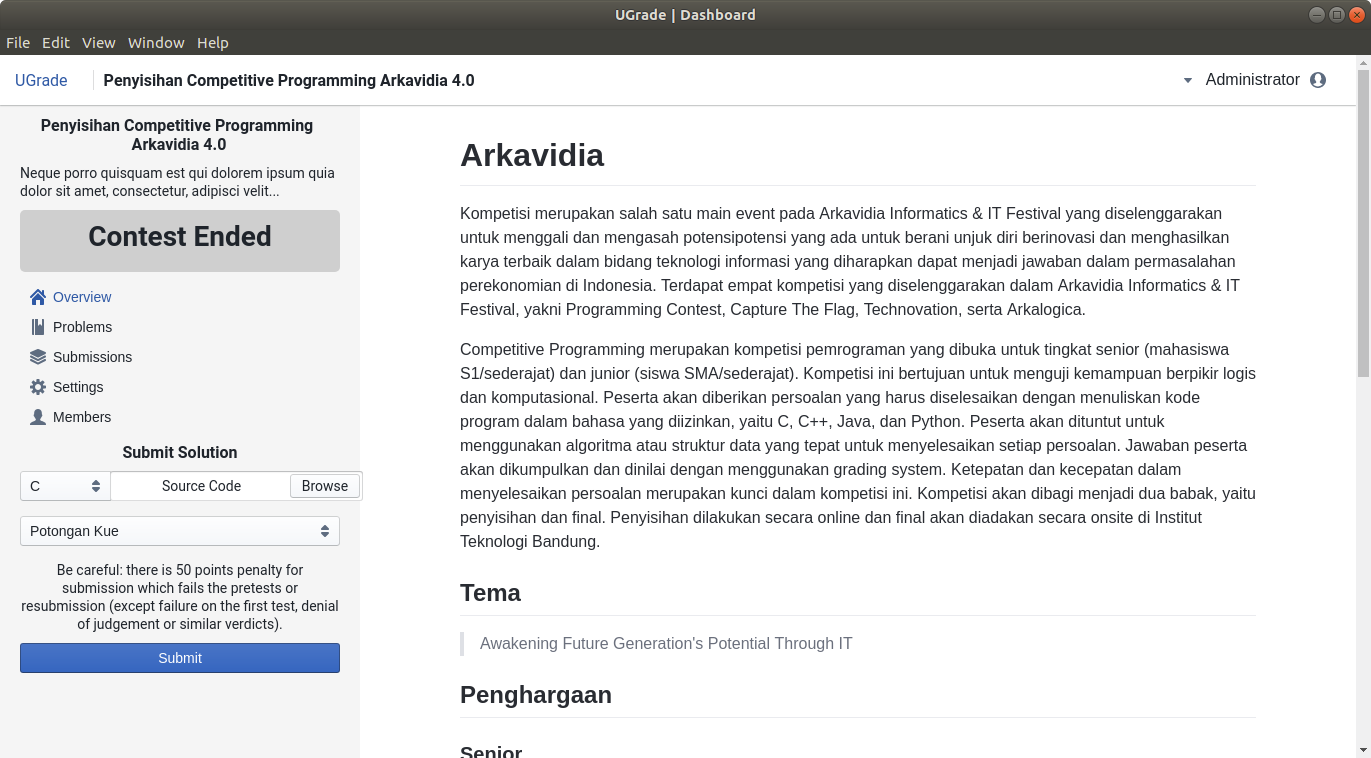
\includegraphics[width=\textwidth]{images/ugdesktop-example}
    \caption{Halaman Kompetisi Dari UGDesktop}
    \label{fig:ugdesktop-example}
\end{figure}

\par UGDesktop dikembangkan menggunakan TypeScript, React, dan Electron. React dipilih karena mudah untuk digunakan dan banyak \textit{library} yang mendukung pengembangan aplikasi berbasis React. React umumnya digunakan untuk mengembangkan aplikasi berbasis \textit{web} dan membutuhkan \textit{web browser} untuk menjalankan aplikasi tersebut. Pengguna membutuhkan aplikasi yang dapat berjalan sebagai aplikasi \textit{desktop} untuk dapat menjalankan sistem antarmuka pengguna sekaligus \textit{worker}. Untuk mengatasi hal tersebut, Electron digunakan untuk menjalankan aplikasi \textit{web} yang berbasis React sebagai aplikasi \textit{desktop}. Gambar \ref{fig:ugdesktop-example} merupakan contoh salah satu halaman pada UGDesktop.

\par Untuk melakukan penilaian, UGDesktop secara periodik menjalankan UGJob. Dalam menjalankan UGJob, UGDesktop menggunakan \textit{token} yang didapatkannya ketika pengguna melakukan \textit{sign in}. UGJob yang dijalankan oleh UGDesktop akan meminta \textit{job} dari UGServer untuk dinilai. UGJob kemudian menilai \textit{job} yang diberikan oleh UGServer dan mengirimkan hasil penilaiannya kembali kepada UGServer.

\section{Pengujian}

\par Pada tugas akhir ini, dilakukan tiga jenis pengujian, yaitu: kinerja, kebenaran dan keamanan. Kinerja dari sistem yang dibangun pada tugas akhir ini diuji dengan melakukan simulasi pengiriman jawaban oleh peserta. Untuk mengukur peningkatan kinerja, sistem \textit{online judge} yang dibangun dibandingkan dengan sistem \textit{online judge} lain yang populer digunakan untuk menyelenggarakan kompetisi \textit{competitive programming}. Kebenaran dari sistem yang dibangun diuji dengan mengirimkan berbagai jenis jawaban kepada sistem. Kebenaran dari sistem ditentukan berdasarkan hasil yang diberikan oleh sistem terhadap berbagai jenis jawaban yang dinilai. Keamanan dari sistem diuji dengan melakukan beberapa jenis serangan kepada sistem. Keamanan dari sisem ditentukan berdasarkan ketahanan sistem terhadap serangan-serangan yang diberikan.

\subsection{Pengujian Kinerja}

\par Pengujian kinerja dilakukan dengan menyimulasikan proses pengiriman jawaban oleh pengguna. Sebuah kompetisi diciptakan dengan beberapa pengguna yang akan mengirimkan jawaban secara periodik. Kinerja sistem yang dibangun dibandingkan dengan sistem \textit{online judge} yang bersifat \textit{open source} yaitu DOMJudge. DOMJudge dipilih karena bersifat \textit{open source} dan sudah populer digunakan untuk menyelenggarakan kompetisi \textit{competitive programming}. DOMJudge telah digunakan untuk menyelenggarakan ACM-ICPC, Arkavidia, Vocompfest dan banyak kompetisi lainnya.

\par Lima belas peserta disiapkan untuk melakukan pengujian terhadap kinerja sistem \textit{online judge} yang akan dibandingkan. Lima belas peserta tersebut akan mengirimkan beberapa \textit{source code} kepada sistem \textit{online judge} secara periodik. Pengujian kinerja ini dilakukan dengan menggunakan sebuah soal \textit{competitive programming}. Soal yang digunakan pada pengujian adalah soal perkalian dua buah polinomial berderajat $N$. Kompleksitas yang diharapkan oleh juri dari soal tersebut adalah $O(N log N)$. Soal ini dipilih karena memiliki beragam solusi dengan kompleksitas yang berbeda-beda. Solusi dengan kompleksitas yang lebih buruk dari $O(N log N)$ akan dianggap sebagai solusi yang salah karena kurang efisien.

\begin{figure}[ht!]
    \centering
    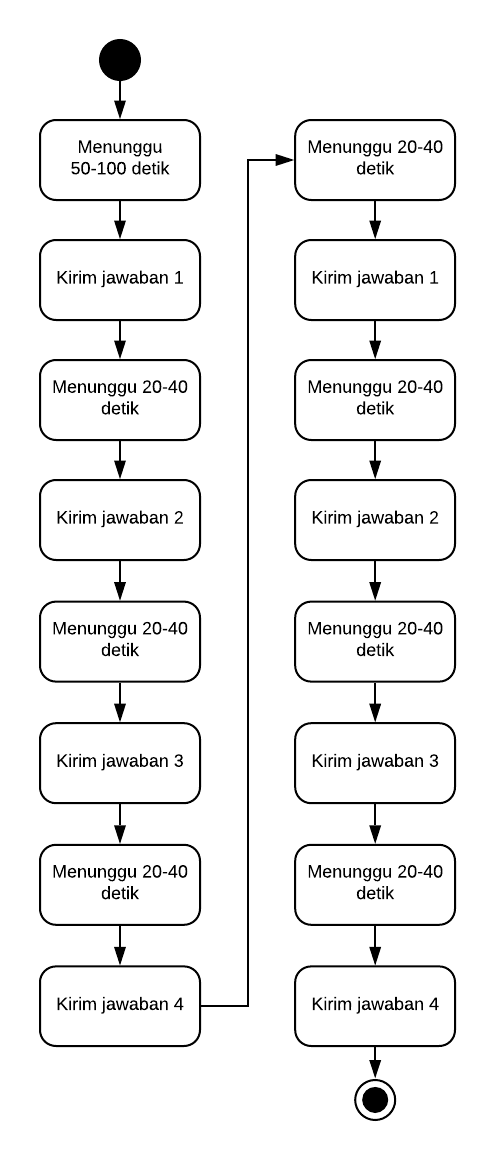
\includegraphics[width=0.5\textwidth]{images/performance-testing-activity}
    \caption{Diagram Aktivitas Dari Pengiriman Jawaban Peserta}
    \label{fig:performance-testing-activity}
\end{figure}

\par Setiap peserta dari lima belas peserta yang telah disiapkan akan menunggu selama lima puluh hingga seratus detik kemudian mengirimkan jawaban secara periodik tiap dua puluh hingga empat puluh detik. Terdapat empat jenis jawaban yang akan dikirimkan oleh peserta, yaitu:
\begin{enumerate}
    \item Jawaban dengan kompleksitas $O(N log N)$. Jawaban ini merupakan jawaban yang diharapkan oleh juri dan akan dinilai sebagai jawaban yang benar.
    \item Jawaban dengan kompleksitas $O(N^{log_2{3}})$.
    \item Jawaban dengan kompleksitas $O(N^2)$.
    \item Jawaban dengan kompleksitas $O(N^2)$ tetapi berbeda implementasi dengan jawaban ketiga.
\end{enumerate}
Setiap peserta akan mengirimkan empat jawaban tersebut secara periodik. Setiap jawaban dari empat jawaban tersebut akan dikirimkan oleh setiap peserta sebanyak dua kali. Jumlah jawaban yang dikirimkan oleh peserta adalah delapan buah jawaban karena setiap peserta mengirimkan setiap jenis jawaban dua kali. Setelah delapan buah jawaban tersebut dikirimkan oleh peserta, peserta akan berhenti mengirimkan jawaban. Diagram aktivitas pada Gambar \ref{fig:performance-testing-activity} menggambarkan alur pengiriman jawaban yang dilakukan oleh setiap peserta.

\par Sistem \textit{online judge} yang akan diuji (DOMJudge dan UGrade) di-\textit{deploy} dengan menggunakan layanan EC2 (\textit{elastic compute cloud}) dari AWS (Amazon Web Service). DOMJudge terdiri dari dua jenis program yaitu DOMServer dan JudgeHost. DOMServer merupakan program yang digunakan oleh DOMJudge sebagai sistem manajemen kompetisi sedangkan JudgeHost merupakan program yang berperan sebagai \textit{autograder}. Pada pengujian kinerja, DOMServer dijalankan pada mesin EC2 dengan tipe \textit{t2.medium}. Mesin tersebut memiliki RAM sebesar 4GB dan dua buah \textit{virtual} CPU. Jenis mesin ini dipilih karena murah dan cukup untuk menangani pengiriman jawaban dari pengguna. JudgeHost dijalankan pada EC2 dengan tipe \textit{t2.micro} yang memiliki 1GB RAM dan satu buah \textit{virtual} CPU. EC2 jenis tersebut dipilih karena murah dan cukup untuk melakukan penilaian jawaban peserta.

\par DOMJudge diuji dengan menjalankan satu buah DOMServer dan dua buah JudgeHost. JudgeHost dijalankan pada dua buah mesin karena umumnya dua buah mesin sudah lebih dari cukup untuk melakukan penilaian jawaban lima belas peserta. Keputusan ini didasari oleh keberjalanan kompetisi \textit{competitive programming} Arkavidia pada tahun 2018 yang diikuti lebih dari seratus orang dengan hanya menggunakan enam buah JudgeHost. Kompetisi tersebut berjalan dengan lancar sehingga dua buah JudgeHost dinilai cukup untuk menilai jawaban dari lima belas orang peserta.

\par Pengujian pada sistem \textit{online judge} dilakukan sebanyak tiga kali. Hal ini bertujuan untuk meningkatkan keakuratan pengujian. Waktu lamanya penilaian sebuah jawaban dan banyaknya antrian jawaban yang ada pada sistem dicatat untuk menentukan kinerja sistem. Tabel \ref{tab:domjudge-wait-time}, \ref{tab:domjudge-process-time} dan \ref{tab:domjudge-system-time} memaparkan data hasil pengujian kinerja sistem \textit{online judge} DOMJudge. Gambar \ref{fig:domjudge-queue} manggambarkan jumlah jawaban yang berada pada antrian sistem DOMJudge dari waktu ke waktu. Terdapat tiga jenis besaran yang dihitung untuk menentukan kinerja DOMJudge, yaitu:
\begin{enumerate}
  \item Waktu tunggu \\ Waktu tunggu didefinisikan sebagai lamanya sebuah jawaban berada pada antrian sistem. Jawaban berada pada antrian sistem mulai dari jawaban tersebut dikirim hingga jawaban tersebut mulai dinilai oleh \textit{autograder}.
  \item Waktu pemrosesan \\ Waktu pemrosesan didefinisikan sebagai lamanya sebuah jawaban dinilai oleh \textit{autograder}. Sebuah jawaban mulai dinilai ketika \textit{worker} dari \textit{autograder} mengambil jawaban tersebut dari antrian sistem.
  \item Waktu penilaian \\ Waktu penilaian didefinisikan sebagai lamanya sebuah jawaban mulai dikirim hingga selesai dinilai. Secara sederhana waktu penilaian merupakan total lamanya sebuah jawaban berada dalam sistem \textit{online judge}. Waktu penilaian juga dapat dipandang sebagai total dari waktu tunggu, waktu pemrosesan dan waktu pengiriman jawaban. Untuk melakukan penilaian, \textit{worker} perlu mengambil jawaban yang ada pada antrian sistem \textit{online judge}. Pengambilan jawaban dari antrian sistem memerlukan waktu karena jawaban perlu dikirimkan melalui jaringan sehingga menimbulkan adanya tambahan waktu yang berupa \textit{network latency}. Pada pengujian yang dilakukan, nilai dari \textit{network latency} sangat kecil dan dapat diabaikan. Karena kecilnya \textit{network latency}, waktu penilaian dapat dipandang sebagai total dari waktu tunggu dan waktu pemrosesan.
\end{enumerate}

\begin{table}[ht]
    \centering
    \begin{tabular}{| c | c | c | c |}
    \hline
    Nomor pengujian & Minimum (detik) & Maksimum (detik) & Rata-rata (detik) \\
    \hline
    \hline
    1 & 0.068 & 384.008 & 188.073 \\
    \hline
    2 & 0.143 & 384.832 & 192.339 \\
    \hline
    3 & 1.3138 & 390.6347 & 194.1095 \\
    \hline
\end{tabular}
    \caption{Data Waktu Tunggu Pada Pengujian Kinerja DOMJudge.}
    \label{tab:domjudge-wait-time}
\end{table}

\begin{table}[ht]
    \centering
    \begin{tabular}{| c | c | c | c |}
    \hline
    Nomor pengujian & Minimum (detik) & Maksimum (detik) & Rata-rata (detik) \\
    \hline
    \hline
    1 & 9.0931 & 12.4293 & 10.011825 \\
    \hline
    2 & 9.0994 & 16.1991 & 10.06895833 \\
    \hline
    3 & 9.0742 & 15.9872 & 10.05397167 \\
    \hline
\end{tabular}
    \caption{Data Waktu Pemrosesan Pada Pengujian Kinerja DOMJudge.}
    \label{tab:domjudge-process-time}
\end{table}

\begin{table}[ht]
    \centering
    \begin{tabular}{| c | c | c | c |}
    \hline
    Nomor pengujian & Minimum (detik) & Maksimum (detik) & Rata-rata (detik) \\
    \hline
    \hline
    1 & 12.3457 & 393.2282 & 198.0845733 \\
    \hline
    2 & 16.3426 & 393.9705 & 202.4083175 \\
    \hline
    3 & 17.301 & 399.7231 & 204.1634717 \\
    \hline
\end{tabular}
    \caption{Data Waktu Penilaian Pada Pengujian Kinerja DOMJudge.}
    \label{tab:domjudge-system-time}
\end{table}

\par Berdasarkan Tabel \ref{tab:domjudge-system-time}, dapat dikatakan bahwa waktu penilaian dari DOMJudge berkisar antara lima belas detik hingga empat ratus detik dengan rata-rata sekitar dua ratus detik. Berdasarkan data tersebut, dapat dikatakan bahwa setiap peserta rata-rata perlu menunggu sekitar tiga hingga empat menit untuk mengetahui nilai dari jawaban yang dikirimkannya. Waktu penilaian ini tergolong tinggi untuk penilaian yang dilakukan oleh \textit{autograder}. Menurut \cite{danutamalms}, waktu penilaian yang dilakukan oleh \textit{autograder} bernilai kurang lebih sepuluh detik. 

\par Waktu penilaian yang tinggi pada pengujian kinerja DOMJudge disebabkan oleh jumlah \textit{worker} yang tidak sebanding dengan jumlah jawaban yang dikirimkan oleh peserta. Umumnya, pada kompetisi \textit{competitive programming}, peserta jarang melakukan pengiriman jawaban dalam rentang waktu yang singkat, akan tetapi pengujian dilakukan dengan cara menyimulasikan peserta untuk mengirimkan jawaban dalam waktu yang singkat. Hal tersebut bertujuan untuk merepresentasikan keadaan dimana peserta kompetisi berjumlah banyak dan jawaban yang harus dinilai oleh sistem berjumlah banyak dalam waktu yang singkat. Sebenarnya pengujian dapat dilakukan dengan cara meningkatkan jumlah peserta, akan tetapi cara tersebut tidak digunakan karena membutuhkan biaya yang besar. Oleh karena itu, pengujian pada tugas akhir ini dilakukan dengan lima belas peserta yang melakukan pengiriman jawaban dalam waktu yang singkat (dua puluh hingga empat puluh detik).

\begin{figure}[ht!]
    \centering
    \begin{tikzpicture}
    \begin{axis}[xlabel={Waktu (detik)}, ylabel={Jumlah jawaban pada antrian}, xmin=0,xmax=700, ymin=0, ymax=100, legend pos=north east, ymajorgrids=true, grid style=dashed,]
        \addplot[color=blue,] table {data/domjudge-queue-test1.txt};
        \addlegendentry{Pengujian pertama}
        \addplot[color=red,] table {data/domjudge-queue-test2.txt};
        \addlegendentry{Pengujian kedua}
        \addplot[color=green] table {data/domjudge-queue-test3.txt};
        \addlegendentry{Pengujian ketiga}
    \end{axis}
\end{tikzpicture}
    \caption{Diagram Jumlah Jawaban Pada Antrian DOMJudge.}
    \label{fig:domjudge-queue}
\end{figure}

% jelasin gambar fig:domjudge-queue
\par Gambar \ref{fig:domjudge-queue} merupakan grafik yang memaparkan jumlah antrian pada DOMJudge seiring berjalannya waktu. Berdasarkan gambar tersebut, puncak jumlah antrian jawaban dari sistem DOMJudge memiliki nilai yang cukup tinggi yaitu tujuh puluh buah jawaban. Dari gambar tersebut terlihat bahwa jumlah antrian pada DOMJudge terus meningkat hingga mencapai suatu puncak tertentu kemudian menurun hingga mencapai angka nol. Terjadinya peningkatan jumlah antrian di awal waktu tersebut disebabkan karena peserta sedang aktif mengirimkan jawaban kepada sistem sedangkan seluruh \textit{worker} sedang sibuk melakukan penilaian. Karena tidak ada \textit{worker} yang tersedia, jawaban peserta terus menerus dimasukkan kedalam antrian sistem dan mengakibatkan jumlah antrian sistem terus meningkat. Tidak tersedianya \textit{worker} tersebut disebabkan karena jumlah \textit{worker} yang tidak sebanding dengan jumlah peserta. Setelah jumlah antrian sistem mencapai puncaknya, jumlah antrian tersebut perlahan-lahan mulai turun. Hal ini disebabkan karena peserta sudah tidak aktif mengirimkan jawaban sehingga jumah antrian tidak bertambah lagi dan mulai turun karena \textit{worker} masih melakukan penilaian pada sisa jawaban di antrian tersebut.  

\par Sistem \textit{online judge} yang dibangun pada tugas akhir ini (UGrade) diuji dengan cara yang sama seperti DOMJudge. Seperti DOMJudge, UGrade juga memiliki dua jenis program yang harus dijalankan yaitu sistem manajemen kompetisi dan \textit{autograder}. Pada UGrade, program yang menjadi sistem manajemen kompetisi adalah UGServer dan program yang menjadi \textit{autograder} adalah UGJob. Pengujian dilakukan dengan menyimulasikan pengiriman jawaban oleh lima belas peserta seperti yang dilakukan pada pengujian DOMJudge.

\par Seperti pada pengujian DOMJudge, sistem manajemen kompetisi UGrade (UGServer) dijalankan pada mesin EC2 yang bertipe \textit{t2.medium}. Karena pada UGrade setiap peserta bertindak sebagai \textit{autograder}, maka pada pengujian ini setiap peserta diberikan sebuah mesin sendiri. Mesin yang digunakan untuk menjalankan \textit{autograder} ini merupakan mesin EC2 yang bertipe \textit{t2.micro}. Mesin tersebut dipilih untuk menyamakan lingkungan \textit{autograder} antara DOMJudge dengan UGrade.

\par Pengujian UGrade dilakukan dengan mengatur \textit{grading size} dengan beberapa nilai. Nilai \textit{grading size} yang digunakan pada pengujian kinerja adalah satu, dua dan lima. Untuk meningkatkan keakuratan pengujian, setiap nilai \textit{grading size} diuji sebanyak tiga kali. Tabel \ref{tab:ugrade-wait-time}, \ref{tab:ugrade-process-time} dan \ref{tab:ugrade-system-time} memaparkan data hasil pengujian kinerja sistem \textit{online judge} UGrade. Gambar \ref{fig:ugrade-queue} manggambarkan jumlah jawaban yang berada pada antrian sistem UGrade dari waktu ke waktu.

\begin{table}[ht!]
    \centering
    \begin{tabular}{| c | c | c | c |}
    \multicolumn{4}{ c }{$\textit{grading size} = 1$} \\
    \hline
    Nomor pengujian & Minimum (detik) & Maksimum (detik) & Rata-rata (detik) \\
    \hline
    1 & 0.042419 & 1.344883 & 0.404296916 \\
    \hline
    2 & 0.042548 & 1.557151 & 0.3983604034 \\
    \hline
    3 & 0.047345 & 1.923494 & 0.4087344167 \\
    \hline

    \multicolumn{4}{ c }{$\textit{grading size} = 2$} \\
    \hline
    Nomor pengujian & Minimum (detik) & Maksimum (detik) & Rata-rata (detik) \\
    \hline
    1 & 0.043881 & 3.361493 & 0.7797795063 \\
    \hline
    2 & 0.046084 & 4.424307 & 0.8150252743 \\
    \hline
    3 & 0.040115 & 3.757078 & 0.8969267395 \\
    \hline

    \multicolumn{4}{ c }{$\textit{grading size} = 5$} \\
    \hline
    Nomor pengujian & Minimum (detik) & Maksimum (detik) & Rata-rata (detik) \\
    \hline
    1 & 0.043896 & 22.403105 & 4.316621826 \\
    \hline
    2 & 0.049549 & 16.500838 & 3.108732139 \\
    \hline
    3 & 0.052324 & 27.276638 & 4.006910664 \\
    \hline
\end{tabular}
    \caption{Data Waktu Tunggu Pada Pengujian Kinerja UGrade}
    \label{tab:ugrade-wait-time}
\end{table}

\par Tabel \ref{tab:ugrade-wait-time} menggambarkan waktu tunggu dari hasil pengujian kinerja UGrade. Berdasarkan tabel tersebut, rata-rata waktu tunggu dari UGrade bergantung pada nilai \textit{grading size}. \textit{Grading size} yang tinggi mengakibatkan nilai dari waktu tunggu menjadi tinggi. Hal tersebut dikarenakan jumlah jawaban yang ada pada antrian sistem menjadi lebih banyak ketika nilai \textit{grading size} tinggi. Jika nilai \textit{grading size} yang dipilih adalah lima, maka setiap jawaban dimasukkan kedalam antrian sistem sebanyak lima kali.

\par Meskipun nilai waktu tunggu pada UGrade tinggi ketika nilai \textit{grading size}-nya tinggi, banyaknya jumlah peserta tidak akan meningkatkan nilai waktu tunggu dari UGrade. Hal tersebut dikarenakan jumlah \textit{worker} juga akan ikut meningkat sesuai dengan peningkatan jumlah peserta. Peningkatan nilai waktu tunggu dari UGrade berbeda dengan DOMJudge. Pada DOMJudge, peningkatan waktu tunggu dipengaruhi oleh jumlah peserta, sedangkan pada UGrade, peningkatan waktu tunggu dipengaruhi oleh nilai \textit{grading size}.

\begin{table}[ht!]
    \centering
    \begin{tabular}{| c | c | c | c |}
    \multicolumn{4}{ c }{$\textit{grading size} = 1$} \\
    \hline
    Nomor pengujian & Minimum (detik) & Maksimum (detik) & Rata-rata (detik) \\
    \hline
    \hline
    1 & 8.401662 & 39.077579 & 12.13586354 \\
    \hline
    2 & 8.411528 & 31.197043 & 11.9722958 \\
    \hline
    3 & 8.364863 & 30.426985 & 11.89300238 \\
    \hline

    \multicolumn{4}{ c }{$\textit{grading size} = 2$} \\
    \hline
    Nomor pengujian & Minimum (detik) & Maksimum (detik) & Rata-rata (detik) \\
    \hline
    \hline
    1 & 8.009209 & 29.991333 & 10.59105839 \\
    \hline
    2 & 8.315464 & 30.062005 & 10.60783176 \\
    \hline
    3 & 8.114838 & 30.923159 & 10.63290684 \\
    \hline

    \multicolumn{4}{ c }{$\textit{grading size} = 5$} \\
    \hline
    Nomor pengujian & Minimum (detik) & Maksimum (detik) & Rata-rata (detik) \\
    \hline
    \hline
    1 & 8.388995 & 28.913371 & 9.896686938 \\
    \hline
    2 & 8.396959 & 29.173359 & 9.882655417 \\
    \hline
    3 & 8.050263 & 29.357337 & 9.698689441 \\
    \hline
\end{tabular}
    \caption{Data Waktu Pemrosesan Pada Pengujian Kinerja UGrade}
    \label{tab:ugrade-process-time}
\end{table}

\par Tabel \ref{tab:ugrade-process-time} memaparkan data waktu pemrosesan jawaban pada UGrade. Berdasarkan tabel tersebut, waktu pemrosesan dari UGrade dapat dikatakan konstan. Waktu pemrosesan dari UGrade tidak bergantung pada jumlah peserta maupun nilai \textit{grading size}. Waktu pemrosesan dari UGrade bergantung pada kinerja komputer yang digunakan untuk menjalankan \textit{worker}. Komputer dengan kinerja yang tinggi akan melakukan penilaian jawaban dengan lebih cepat dan mengakibatkan turunnya nilai waktu pemrosesan. Berdasarkan hasil pengujian, rata-rata dari waktu pemrosesan UGrade kurang lebih adalah sepuluh detik. Berdasarkan Tabel \ref{tab:domjudge-process-time} dan \ref{tab:ugrade-process-time}, nilai waktu pemrosesan dari UGrade memiliki kesamaan dengan waktu pemrosesan DOMJudge. Hal tersebut dikarenakan mesin yang digunakan untuk melakukan pengujian pada UGrade dan DOMJudge adalah mesin dengan kinerja yang sama.

\begin{table}[ht!]
    \centering
    \begin{tabular}{| c | c | c | c |}
    \multicolumn{4}{ c }{$\textit{grading size} = 1$} \\
    \hline
    Nomor pengujian & Minimum (detik) & Maksimum (detik) & Rata-rata (detik) \\
    \hline
    \hline
    1 & 8.525866 & 40.033336 & 12.54016045 \\
    \hline
    2 & 8.454445 & 31.536312 & 12.3706562 \\
    \hline
    3 & 8.445607 & 31.41732 & 12.3017368 \\
    \hline

    \multicolumn{4}{ c }{$\textit{grading size} = 2$} \\
    \hline
    Nomor pengujian & Minimum (detik) & Maksimum (detik) & Rata-rata (detik) \\
    \hline
    \hline
    1 & 8.140914 & 32.316424 & 11.3708379 \\
    \hline
    2 & 8.418419 & 31.976166 & 11.42285704 \\
    \hline
    3 & 8.367557 & 33.021025 & 11.52983358 \\
    \hline

    \multicolumn{4}{ c }{$\textit{grading size} = 5$} \\
    \hline
    Nomor pengujian & Minimum (detik) & Maksimum (detik) & Rata-rata (detik) \\
    \hline
    \hline
    1 & 8.538458 & 34.79008 & 14.21330876 \\
    \hline
    2 & 8.558542 & 34.040856 & 12.99138756 \\
    \hline
    3 & 8.260255 & 35.796819 & 13.70560011 \\
    \hline
\end{tabular}
    \caption{Data Waktu Penilaian Pada Pengujian UGrade}
    \label{tab:ugrade-system-time}
\end{table}

\par Tabel \ref{tab:ugrade-system-time} memaparkan data waktu penilaian jawaban pada UGrade. Pada tabel tersebut, terlihat bahwa nilai \textit{grading size} hanya sedikit memengaruhi waktu penilaian jawaban pada UGrade. Nilai waktu penilaian dapat dipandang sebagai total dari waktu pemrosesan dan waktu tunggu. Berdasarkan Tabel \ref{tab:ugrade-process-time} dan \ref{tab:ugrade-wait-time}, waktu pemrosesan UGrade dapat dikatakan jauh lebih tinggi dibanding waktu tunggu-nya. Hal tersebut mengakibatkan nilai waktu penilaian hanya sedikit dipengaruhi oleh waktu tunggu. Pada Tabel \ref{tab:ugrade-system-time} terlihat bahwa waktu penilaian dari UGrade dengan nilai \textit{grading size} lima memiliki rata-rata sekitar tiga belas detik. Angka tersebut dapat dipandang sebagai penjumlahan dari waktu tunggu UGrade yang memiliki rata-rata sekitar empat detik dan waktu pemrosesan yang memiliki rata-rata sekitar sembilan detik.

\par Berdasarkan Tabel \ref{tab:domjudge-system-time} dan \ref{tab:ugrade-system-time}, waktu penilaian pada DOMJudge dan UGrade memiliki perbedaan yang sangat signifikan. Pada DOMJudge, rata-rata waktu penilaiannya bernilai hingga dua ratus detik, sedangkan pada UGrade rata-rata waktu penilaiannya bernilai sekitar tiga belas detik. Pada DOMJudge, peserta harus menunggu sekitar tiga menit untuk mendapatkan hasil dari penilaian jawabannya, sedangkan pada UGrade peserta hanya perlu menunggu sekitar tiga belas detik saja. Hal ini disebabkan karena jumlah \textit{worker} pada DOMJudge tidak sebanding dengan jumlah jawaban yang dikirimkan oleh peserta, sedangkan pada UGrade jumlah \textit{worker} mengikuti jumlah peserta.

\begin{figure}[ht!]
    \centering
    \begin{tikzpicture}
    \begin{groupplot}[group style={group size=1 by 3}, xmin=0,xmax=1000, ymin=0, ymax=20, legend pos=north east, ymajorgrids=true, grid style=dashed, height=0.3\textwidth, width=\textwidth]
        \nextgroupplot
        \addplot[color=green,] table {data/ugrade-queue-gz5-test1.txt}; \label{plots:ugrade-queue-gz5}
        \addplot[color=red,] table {data/ugrade-queue-gz2-test1.txt}; \label{plots:ugrade-queue-gz2}
        \addplot[color=blue,] table {data/ugrade-queue-gz1-test1.txt}; \label{plots:ugrade-queue-gz1}
        \coordinate (top) at (rel axis cs:0,1);% coordinate at top of the first plot
        
        \nextgroupplot[ylabel={Jumlah jawaban pada antrian}]
        \addplot[color=green,] table {data/ugrade-queue-gz5-test2.txt};
        \addplot[color=red,] table {data/ugrade-queue-gz2-test2.txt};
        \addplot[color=blue,] table {data/ugrade-queue-gz1-test2.txt};
        
        \nextgroupplot[xlabel={Waktu (detik)}]
        \addplot[color=green,] table {data/ugrade-queue-gz5-test3.txt};
        \addplot[color=red,] table {data/ugrade-queue-gz2-test3.txt};
        \addplot[color=blue] table {data/ugrade-queue-gz1-test3.txt};
        \coordinate (bot) at (rel axis cs:1,0);% coordinate at bottom of the last plot
    \end{groupplot}

    \path (top|-current bounding box.north)--
      coordinate(legendpos)
      (bot|-current bounding box.north);
    \matrix[matrix of nodes,anchor=south,draw,inner sep=0.2em,draw]
        at([yshift=1ex]legendpos) {
            \ref{plots:ugrade-queue-gz5}& $\textit{grading size} = 5$ &[5pt]
            \ref{plots:ugrade-queue-gz2}& $\textit{grading size} = 2$ &[5pt]
            \ref{plots:ugrade-queue-gz1}& $\textit{grading size} = 1$ \\
        };
\end{tikzpicture}
    \caption{Diagram Jumlah Jawaban Pada Antrian UGrade Dengan Tiga Kali Pengujian}
    \label{fig:ugrade-queue}
\end{figure}

% jelasin gambar fig:ugrade-queue
\par Berdasarkan Gambar \ref{fig:ugrade-queue}, jumlah antrian dari sistem UGrade bergantung pada nilai \textit{grading size}. \textit{Grading size} yang tinggi menybabkan jumlah antrian pada sistem menjadi tinggi pula. \textit{Grading size} yang tinggi menybabkan sebuah jawaban harus dinilai beberapa kali sehingga jumlah antrian pada sistem meningkat. Kinerja dari UGrade dapat ditingkatkan dengan memilih nilai \textit{grading size} yang rendah. Meskipun begitu, nilai \textit{grading size} yang rendah akan mengurangi tingkat keamanan dari UGrade. Juri perlu menentukan nilai \textit{grading size} yang tepat untuk mendapatkan hasil yang optimal. Nilai \textit{grading size} perlu dipilih sedemikian rupa sehingga cukup tinggi untuk menjamin keamanan kompetisi dan cukup rendah untuk dapat memberikan kinerja yang optimal.

% jelasin perbedaan fig:domjudge-queue sama fig:ugrade-queue
\par Berbeda dengan jumlah antrian pada DOMJudge, jumlah antrian pada UGrade jauh lebih rendah dibandingkan dengan DOMJudge. Hal ini dikarenakan jumlah \textit{worker} yang ada pada DOMJudge selalu tetap dan tidak bergantung pada jumlah peserta, sedangkan jumlah \textit{worker} pada UGrade akan mengikuti jumlah peserta yang ada pada kompetisi tersebut. Pada pengujian yang dilakukan, jumlah \textit{worker} pada DOMJudge jauh lebih kecil dibandingkan dengan jumlah peserta kompetisi sehingga jumlah antrian pada sistem DOMJudge mengalami kenaikan di awal waktu dan memiliki puncak yang cukup tinggi. Grafik antrian pada UGrade tidak memiliki kenaikan yang signifikan maupun puncak yang tinggi. Hal tersebut dikarenakan jumlah \textit{worker} pada UGrade akan mengikuti banyaknya peserta pada kompetisi tersebut sehingga beban dari setiap \textit{worker} akan cenderung konstan berapapun pesertanya.

\subsection{Pengujian Kebenaran}

\par Selain pengujian kinerja, diperlukan pengujian kebenaran dari sistem yang dibangun. Pengujian kebenaran dilakukan dengan menyimulasikan proses pengiriman jawaban oleh peserta. Kebenaran sistem yang dibangun ditentukan berdasarkan \textit{verdict} penilaian yang diberikan oleh sistem. Sistem yang benar akan memberikan \textit{verdict} yang sama ketika jawaban yang sama dinilai berkali-kali di komputer yang berbeda. Pada pengujian kebenaran, digunakan sebuah soal dengan enam buah jawaban yang diharapkan akan memiliki \textit{verdict} \textit{accepted}, \textit{wrong answer}, \textit{memory limit exceeded}, \textit{time limit exceeded}, \textit{runtime error}, dan \textit{compile error}.

\par Pengujian kebenaran dilakukan dengan mengirimkan berbagai jenis jawaban kepada sistem UGrade. Soal yang digunakan untuk melakukan pengujian merupakan soal perkalian polinomial berderajat seratus ribu. Soal tersebut didapatkan dari kompetisi Arkavidia 2018. Soal tersebut dipilih karena memiliki solusi yang beraneka ragam dengan kompleksitas yang berbeda-beda. Kompleksitas yang diharapkan dari soal tersebut adalah $O(N log N)$.

\par Tujuh jenis jawaban dikirimkan ke sistem UGrade untuk menguji kebenaran dari sistem. Tujuh jenis jawaban tersebut adalah sebagai berikut:
\begin{enumerate}
	\item Jawaban yang diinginkan oleh juri, yaitu jawaban dengan kompleksitas $O(N log N)$.
	\item Jawaban dengan kompleksitas $O(N^{log_2{3}})$. Jawaban ini memiliki kompleksitas yang lebih buruk dari jawaban yang diharapkan oleh juri dan dianggap sebagai jawaban yang salah karena tidak berjalan dengan cukup cepat.
	\item Jawaban dengan kompleksitas $O(N^2)$. Seperti pada jenis jawaban ke-dua, jawaban ini dinilai tidak cukup cepat untuk persoalan yang diberikan.
	\item Jawaban dengan kompleksitas $O(N^2)$. Jawaban ini memiliki kompleksitas yang sama seperti pada jawaban jenis ketiga tetapi memiliki implementasi yang berbeda.
	\item Jawaban dengan penggunaan memori yang terlalu banyak. Jawaban ini menggunakan memori yang melebihi batasan dari juri.
	\item Jawaban yang menimbulkan adanya \textit{runtime error} karena ada pengaksesan memori yang belum dialokasikan.
	\item Jawaban yang memiliki kesalahan penulisan dan tidak dapat dikompilasi.
\end{enumerate}
Jawaban tersebut akan dikirimkan ke sistem UGrade. \textit{Verdict} yang diberikan oleh UGrade dicatat untuk menentukan kebenaran dari program UGrade. Untuk meningkatkan akurasi, setiap jenis jawaban dikirimkan sebanyak lima puluh kali. Jawaban yang sama harus memiliki \textit{verdict} yang sama jika dinilai berkali-kali.

\par Pengujian dilakukan pada komputer dengan \textit{clock speed} 2.5GHz dan RAM 8GB. Hasil pengujian tersebut adalah sebagai berikut:
\begin{enumerate}
	\item UGrade menghasilkan \textit{verdict} \textit{accepted} untuk seluruh jawaban jenis pertama yang dikirimkan.
	\item UGrade menghasilkan \textit{verdict} \textit{time limit exceeded} untuk seluruh jawaban jenis ke-dua yang dikirimkan.
	\item UGrade menghasilkan \textit{verdict} \textit{time limit exceeded} untuk seluruh jawaban jenis ke-tiga yang dikirimkan.
	\item UGrade menghasilkan \textit{verdict} \textit{time limit exceeded} untuk seluruh jawaban jenis ke-empat yang dikirimkan.
	\item UGrade menghasilkan \textit{verdict} \textit{memory limit exceeded} untuk seluruh jawaban jenis ke-lima yang dikirimkan.
	\item UGrade menghasilkan \textit{verdict} \textit{runtime error} untuk seluruh jawaban jenis ke-enam yang dikirimkan.
	\item UGrade menghasilkan \textit{verdict} \textit{compile error} untuk seluruh jawaban jenis ke-tujuh yang dikirimkan.
Hasil pengujian tersebut sesuai yang diharapkan. Oleh karena itu, berdasarkan hasil pengujian tersebut, sistem \textit{online judge} UGrade dapat dikatakan lolos uji kebenaran.

\end{enumerate}

\subsection{Pengujian Keamanan}
\par Sistem \textit{online judge} yang dibangun perlu memiliki tingkat keamanan yang cukup sehingga tidak membahayakan komputer peserta dan sistem. Pengujian keamanan dilakukan dengan menyimulasikan pengiriman jawaban yang berbahaya ke sistem \textit{online judge}. Pengujian keamanan dilakukan dengan mengirimkan lima jenis jawaban yang berbahaya, yaitu:
\begin{enumerate}
    \lstinputlisting[caption={\textit{Fork Bomb}},label={lst:prog-fork-bomb},language=C,style=CStyle]{listings/fork-bomb.cpp}
    \item Jawaban yang berisi \textit{fork bomb} seperti pada Kode \ref{lst:prog-fork-bomb}.
    \lstinputlisting[caption={\textit{Compile Bomb}},label={lst:prog-compile-bomb},language=C,style=CStyle]{listings/compile-bomb.c}
    \item Jawaban yang berisi \textit{compile bomb} seperti pada Kode \ref{lst:prog-compile-bomb}.
    \lstinputlisting[caption={\textit{Program Yang Mencoba Keluar Dari Lingkungan \textit{Chroot}}},label={lst:prog-chroot-break},language=C,style=CStyle]{listings/chroot-break.c}
    \item Jawaban yang mencoba keluar dari lingkungan \textit{sandbox} seperti pada Kode \ref{lst:prog-chroot-break}.
    \lstinputlisting[caption={\textit{\textit{Sleeping Program}}},label={lst:prog-timelimit},language=C,style=CStyle]{listings/busy-sleep.c}
    \item Jawaban yang hanya melakukan \textit{sleep} seperti pada Kode \ref{lst:prog-timelimit}.
    \lstinputlisting[caption={Program Dengan IO yang besar},label={lst:prog-huge-io},language=C,style=CStyle]{listings/huge-io.cpp}
    \item Jawaban yang menghasilkan \textit{file} yang sangat besar seperti pada Kode \ref{lst:prog-huge-io}.
\end{enumerate} 
\textit{Worker} yang menjalankan lima jenis jawaban tersebut harus dapat menghentikan proses penilaian karena jawaban tersebut berpotensi menimbulkan kerusakan pada \textit{worker}. Komputer yang bertindak sebagai worker diharapkan dapat tetap berjalan setelah jawaban tersebut dieksekusi. Keamanan dari UGrade ditentukan berdasarkan adanya efek samping yang muncul setelah jawaban-jawaban tersebut dieksekusi. Jika tidak ada efek samping yang muncul setelah jawaban tersebut dieksekusi, maka sistem UGrade dikatakan lolos uji keamanan. 

\par Pengujian dilakukan menggunakan komputer yang memiliki empat buah \textit{core} CPU dengan \textit{clock speed} 2.5GHz dan memiliki RAM sebesar 8GB. Hasil dari pengujian yang dilakukan adalah sebagai berikut:
\begin{enumerate}
  \item \textit{Worker} berhasil menghentikan program solusi peserta yang mengandung \textit{fork bomb} dan memberikan \textit{verdict} \textit{time limit exceeded}. Hal tersebut dikarenakan program peserta hanya melakukan pemanggilan \textit{system call fork} secara terus menerus tanpa pernah berhenti sehingga \textit{worker} menganggap program tersebut menghabiskan \textit{resource} CPU. Pemanggilan \textit{system call} \textit{fork} berhasil digagalkan oleh \textit{worker} karena jumlah proses yang berada dalam lingkungan \textit{sandbox} sudah dibatasi menggunakan \textit{system call} \textit{setrlimit}.
  \item \textit{Worker} berhasil menghentikan program solusi peserta yang berisi \textit{compile bomb} dan memberikan \textit{verdict} \textit{compile error}. Proses kompilasi kode program solusi peserta menghabiskan banyak memori dan \textit{disk space} sehingga \textit{worker} menghentikan proses kompilasi secara paksa. \textit{Worker} mengetahui penggunaan memori proses kompilasi dengan menggunakan fitur \textit{cgroup} yang ada pada Linux. Dengan mengetahui penggunaan memori dari proses kompilasi, \textit{worker} dapat menghentikan proses kompilasi tersebut secara paksa ketika penggunaan memorinya dinilai sudah berlebihan. Selain itu, \textit{worker} juga menggunakan \textit{system call setrlimit} untuk membatasi ukuran \textit{file} yang dihasilkan oleh proses kompilasi. 
  \item \textit{Worker} berhasil melindungi komputer yang digunakan sebagai \textit{worker} terhadap program solusi peserta yang mencoba keluar dari lingkungan \textit{sandbox}. Kode yang digunakan untuk melakukan pengujian ini adalah Kode \ref{lst:prog-chroot-break}. Jika serangan tersebut berhasil dilakukan, maka akan tercipta \textit{file breakout} pada direktori \textit{/tmp}. Setelah pengujian dilakukan, \textit{file} tersebut tidak ditemukan pada direktori \textit{/tmp} sehingga dapat dikatakan serangan yang dilakukan tidak berhasil.
  \item \textit{Worker} berhasil menghentikan program solusi peserta yang hanya melakukan \textit{sleep} tanpa menggunakan banyak \textit{resource}. Meskipun program tersebut hanya melakukan \textit{sleep} dan tidak menggunakan CPU secara berlebihan, \textit{worker} dapat menghentikan program tersebut karena telah membatasi nilai \textit{wall-clock time} dari program tersebut.
  \item \textit{Worker} berhasil menghentikan program solusi peserta yang menggunakan IO secara berlebihan dan menghasilkan \textit{file} yang sangat besar. Hal ini dicapai oleh \textit{worker} dengan memanfaatkan \textit{system call setrlimit} yang ada pada Linux. Dengan menggunakan \textit{setrlimit}, ukuran \textit{file} yang dapat dibuat oleh sebuah proses pada Linux dapat dibatasi.
\end{enumerate}

\par Berdasarkan hasil pengujian pada paragraf sebelumnya, tidak ditemukan adanya kerusakan maupun efek samping yang muncul pada sistem \textit{online judge} maupun \textit{worker}. Hal tersebut mengindikasikan bahwa serangan yang dilakukan oleh peserta tidak berhasil merusak sistem \textit{online judge} maupun \textit{worker}. Oleh karena itu, dapat dikatakan sistem \textit{online judge} yang dibangun pada tugas akhir ini lolos uji keamanan.

% \par Kerahasiaan dan integritas dari \textit{testcase}, solusi juri dan solusi peserta perlu dijaga. Untuk menjaga kerahasiaan dan integritas, diperlukan adanya pengujian. Pengujian integritas dilakukan dengan melakukan percobaan merusak \textit{testcase}, solusi juri dan solusi peserta yang ada pada komputer \textit{worker}. Perusakan pada \textit{testcase}, solusi juri ataupun solusi peserta diharapkan dapat dikenali dan diatasi sehingga hasil penilaian dari \textit{worker} akan tetap benar. Kerahasiaan \textit{testcase}, solusi juri dan solusi peserta hanya akan diuji dengan melihat isi dari \textit{file} \textit{testcase}, solusi juri dan solusi peserta. Kerahasiaan akan dianggap lolos uji jika isi dari \textit{file} \textit{testcase}, solusi juri maupun solusi peserta tidak dapat dibaca oleh pengguna.

% TODO: data pengujian

    \chapter{Simpulan dan Saran}

% TODO: tambah kasus ICPC, yang ditanyain turfa waktu seminar 2

\par Terdapat beberapa kesimpulan dan saran terkait pengembangan dan hasil pada tugas akhir ini. Pada bab ini diberikan kesimpulan dari tugas akhir dan saran pengembangan lebih lanjut terhadap solusi yang sudah dipaparkan.

\section{Simpulan}

\par Pada tugas akhir ini telah dikembangkan sistem \textit{online judge} yang bernama UGrade. Beberapa kesimpulan yang didapatkan pada pengerjaan tugas akhir ini antara lain adalah:
\begin{enumerate}
    \item Terdapat peningkatan kinerja penilaian yang cukup tinggi pada UGrade dibandingkan dengan sistem \textit{online judge} yang saat ini populer digunakan dalam menyelenggarakan \textit{competitive programming}. Peningkatan kinerja ini terjadi karena jumlah \textit{worker} pada UGrade berbanding lurus dengan jumlah jawaban yang perlu dinilai. Hal ini terjadi karena jumlah \textit{worker} mengikuti jumlah peserta sehingga berbanding lurus pula dengan jumlah jawaban yang perlu dinilai.
    \item Kinerja penilaian sistem \textit{online judge} UGrade tidak dipengaruhi oleh jumlah peserta, akan tetapi dipengaruhi oleh nilai \textit{grading size} dari kompetisi. Jumlah peserta tidak memengaruhi kinerja penilaian UGrade karena jumlah \textit{worker} mengikuti jumlah peserta sehingga akan tetap berbanding lurus dengan jumlah jawaban yang perlu dinilai. Meskipun begitu, perbedaan nilai \textit{grading size} menimbulkan perbedaan jumlah jawaban yang perlu dinilai karena jumlah jawaban akan berlipat ganda sesuai dengan nilai dari \textit{grading size}.
    \item Nilai \textit{grading size} yang tinggi mengakibatkan berkurangnya kinerja penilaian sistem \textit{online judge} UGrade akan tetapi meningkatkan keamanannya. Begitu juga sebaliknya, nilai \textit{grading size} yang rendah meningkatkan kinerja penilaian tetapi mengurangi tingkat keamanannya.
    \item Berdasarkan hasil pengujian keamanan, kemanan dari sistem \textit{online judge} UGrade cukup untuk menyelenggarakan kompetisi \textit{competitive programming}. Meskipun UGrade masih tidak dapat menangani serangan \textit{reverse engineering}, akan tetapi UGrade aman digunakan untuk menyelenggarakan kompetisi \textit{competitive programming} yang bersifat \textit{onsite} seperti ACM-ICPC dimana komputer peserta disediakan oleh juri.
    \item UGrade dapat menjaga keadilan penilaian meskipun komputer \textit{worker} memiliki spesifikasi yang berbeda-beda. Hal ini dicapai dengan cara membandingkan hasil eksekusi solusi juri dan eksekusi solusi peserta pada komputer \textit{worker}.
    \item Teknik \textit{load balancing} yang digunakan oleh UGrade menyebabkan beban UGServer menjadi sangat berat karena \textit{worker} selalu mengirimkan \textit{request} kepada \textit{server} secara periodik.
    \item Terdapat kasus yang masih belum bisa ditangani secara akurat oleh sistem \textit{sandbox} UGrade yaitu pembatasan jumlah proses yang berjalan dalam lingkungan \textit{sandbox} dan pembatasan hak akses terhadap \textit{file} yang ada dalam lingkungan \textit{sandbox}.
\end{enumerate}

% \par Pada tugas akhir ini telah diciptakan sistem \textit{online judge} yang bernama \textit{UGrade}. \textit{UGrade} memanfaatkan komputer pengguna untuk menjadi \textit{worker} dalam melakukan penilaian jawaban peserta kompetisi. Berdasarkan hasil pengujian, penggunaan komputer pengguna sebagai \textit{worker} meningkatkan kinerja penilaian. Hal ini dikarenakan jumlah \textit{worker} yang melakukan penilaian sebanding dengan jumlah peserta yang mengirimkan \textit{jawaban}.

% \par Pada tugas akhir ini telah diciptakan sistem \textit{online judge} yang bernama UGrade. UGrade memanfaatkan komputer pengguna untuk menjadi \textit{worker} dalam melakukan penilaian jawaban peserta kompetisi. Berdasarkan hasil pengujian, UGrade memiliki kinerja penilaian jawaban peserta yang lebih tinggi dibandingkan sistem \textit{online judge} yang saat ini populer digunakan. Pada sistem \textit{online judge} UGrade, kinerja dari proses penilaian jawaban peserta dipengaruhi oleh nilai \textit{grading size} yang digunakan dalam kompetisi. Nilai \textit{grading size} yang tinggi akan mengurangi kinerja dari proses penilaian, akan tetapi dapat meningkatkan keamanan sistem. Begitu juga sebaliknya, nilai \textit{grading size} yang rendah meningkatkan kinerja penilaian, akan tetapi dapat mengurangi keamanan sistem. Juri perlu mengatur nilai \textit{grading size} sehingga proses penilaian cukup aman dan memiliki kinerja yang tinggi.

% \par Dalam kompetisi \textit{competitive programming}, peserta mungkin saja melakukan serangan yang mengakibatkan kerusakan pada sistem \textit{online judge}. Keamanan dari sistem \textit{online judge} yang dibangun perlu diuji untuk menentukan ketahanannya terhadap serangan dari peserta. Pengujian terhadap serangan yang mungkin dilakukan oleh peserta dilakukan dengan mengirimkan jawaban yang bebahaya kepada sistem yang dibangun. Keamanan dari UGrade ditentukan berdasarkan adanya efek samping yang muncul ketika jawaban peserta dinilai. Berdasarkan pengujian yang telah dilakukan, tidak ada efek samping yang muncul setelah jawaban peserta yang berbahaya dinilai. Oleh karena itu, sistem UGrade dapat dikatakan cukup aman untuk digunakan dalam kompetisi \textit{competitive programming}.

% \par Kebenaran dari sistem \textit{online judge} UGrade diuji dengan mengirimkan beberapa jenis jawaban secara berulang-ulang kepada sistem. Kebenaran dari sistem UGrade ditentukan berdasarkan \textit{verdict} yang diberikan oleh sistem terhadap jawaban-jawaban tersebut. Pengujian ini dilakukan dengan menggunakan tujuh jenis jawaban yang berbeda. Berdasarkan hasil pengujian, UGrade memberikan \textit{verdict} yang benar kepada seluruh jawaban yang dikirimkan oleh peserta.

% \par Sistem \textit{online judge} UGrade masih belum dapat menangani serangan yang berupa \textit{reverse engineering}. Peserta yang memiliki akses \textit{root} dari komputer yang digunakannya dapat melakukan serangan terhadap sistem dengan mengubah kode program \textit{autograder} dari UGrade. Meskipun begitu, untuk beberapa jenis kompetisi \textit{competitive programming}, serangan ini dapat diatasi dengan tidak memberikan akses \textit{root} kepada peserta. Kompetisi ACM-ICPC merupakan salah satu jenis kompetisi yang dapat bertahan dari serangan \textit{reverse engineering}.

% \par Pada kompetisi ACM-ICPC, peserta umumnya akan diseleksi terlebih dahulu secara bertingkat sebelum akhirnya berkompetisi di \textit{world final}. Sebelum babak \textit{world final}, jumlah peserta yang mengikuti kompetisi relatif sedikit sehingga sistem \textit{online judge} yang saat ini sering digunakan cukup untuk menjalankan kompetisi tersebut. Pada \textit{world final}, jumlah peserta kompetisi menjadi sangat banyak karena terdiri dari peserta-peserta yang lolos dari berbagai negara. Pada \textit{world final}, juri akan memberikan komputer khusus kepada peserta untuk mengikuti kompetisi tersebuti. Pada babak \textit{world final}, juri dapat menggunakan sistem \textit{online judge} UGrade untuk menilai jawaban peserta. Juri dapat mengatur agar peserta tidak mendapatkan akses \textit{root} pada komputer yang digunakannya sehingga tidak dapat melakukan berbagai jenis serangan yang berupa \textit{reverse engineering}.

% \par Teknik \textit{load balancing} yang digunakan oleh UGrade mengikuti teknik \textit{load balancing} yang digunakan oleh sistem \textit{online judge} yang saat ini populer digunakan yaitu \textit{pull-based load balancing}. Teknik \textit{load balancing} ini ternyata tidak terlalu baik digunakan jika jumlah \textit{worker} sangat banyak. \textit{Worker} yang banyak mengakibatkan banyaknya \textit{request} yang harus ditangani oleh \textit{server} sehingga \textit{server} menjadi mudah gagal. Hal ini tidak ditemukan pada sistem \textit{online judge} yang saat ini populer digunakan. Hal tersebut dikarenakan umumnya sistem \textit{online judge} yang saat ini populer digunakan tidak menggunakan banyak \textit{worker} untuk melakukan penilaian.

% \par Sistem \textit{sandbox} yang digunakan pada UGrade dibangun dengan bahasa Go dan diberi nama UGSbox. Saat ini, UGSbox dapat memberikan isolasi yang cukup baik untuk mengeksekusi program yang dikirimkan oleh peserta. Meskipun begitu, masih terdapat beberapa kekurangan pada UGSbox karena dibangun dengan bahasa Go. Salah satu kekurangan UGSbox adalah tidak bisa membatasi jumlah proses yang diciptakan oleh proses yang diisolasi secara akurat. Hal ini disebabkan bahasa Go memiliki \textit{runtime} yang perlu dijalankan sebagai proses tersendiri sehingga UGSbox sulit untuk membatasi jumlah proses yang harus diisolasi. Selain itu, \textit{resource} yang digunakan oleh \textit{go runtime} juga ikut dihitung dalam membatasi \textit{resource} proses yang diisolasi. Hal tersebut mengakibatkan pembatasan \textit{resource} yang digunakan oleh proses yang diisolasi menjadi kurang akurat.

\section{Saran}

\par Terdapat beberapa kekurangan pada pengerjaan tugas akhir ini. Berikut beberapa saran yang dapat diberikan untuk pengerjaan tugas akhir ini:
\begin{enumerate}
    \item Pemilihan teknik penilaian membutuhkan adanya studi lebih lanjut. Jika banyak peserta melakukan serangan terhadap sistem, \textit{self grading} dapat mengurangi risiko terjadinya kerusakan sistem. Sistem \textit{online judge} dapat dibuat untuk mudah dikonfigurasi (\textit{configurable}) sehingga dapat menggunakan beberapa jenis sistem penilaian.
    \item UGDesktop berukuran sangat besar karena mengguna \textit{framework} React dan Electron. Aplikasi \textit{desktop} dapat dibuat lebih \textit{native} dengan menggunakan \textit{library} seperti GTK.
    \item Pemilihan \textit{framework} Django untuk bertindak sebagai \textit{server} tidak dapat menangani banyaknya pengguna dengan efisien. Bahasa Go dapat digunakan untuk meningkatkan kinerja dari \textit{server}.
    \item Karena setiap peserta berperan sebagai \textit{worker}, jumlah \textit{request} yang perlu ditangani oleh UGServer sangat banyak dan memberatkan UGServer. Hal tersebut dikarenakan metode yang digunakan untuk \textit{load balancing} adalah \textit{pull-based load balancing} sehingga setiap \textit{worker} terus menerus mengirim \textit{request} kepada \textit{server}. Metode \textit{load balancing} perlu dimodifikasi sehingga beban \textit{server} dapat berkurang.
    \item Penggunaan bahasa Go untuk mengembangkan lingkungan \textit{sandbox} kurang efektif. Bahasa Go sulit untuk melakukan \textit{system call fork} dan \textit{exec} secara terpisah karena adanya \textit{go runtime} yang perlu dijalankan. \textit{Sandbox} dapat dikembangkan dengan bahasa yang lebih \textit{low-level} seperti C, C++ atau Rust. 
    \item Penggunaan istilah \textit{grading group}, \textit{grading size}, \textit{grading} dan \textit{grader group} sulit dipahami. Penggunaan nama yang mirip sebaiknya dihindari dengan memilih nama yang lebih deskriptif dan tidak terlalu mirip. 
    \item Bahasa yang didukung oleh UGrade masih terbatas C dan C++. UGrade perlu memberikan dukungan terhadap bahasa Pascal, Python dan Java karena bahasa tersebut sering digunakan pada kompetisi \textit{competitive programming}.
\end{enumerate}


    \renewcommand\bibname{DAFTAR PUSTAKA}
    \printbibliography

\end{document}
